\graphicspath{{figures/chapter4/}}
\onehalfspacing

\chapter{Deep learning low-cost photogrammetry for 4D short-term glacier monitoring
  (2022-2023)}\label{ch:4}

% \vfill
% \vspace{5mm}

\newthought{This chapter is based on:}

\begin{itemize}
  \item Ioli, F., Dematteis, N., Giordan, D., Nex, F., Pinto, L. (2024). Deep Learning Low-cost Photogrammetry for 4D Short-term Glacier Dynamics Monitoring. \textit{PFG}, \footnotesize{\url{https://doi.org/10.1007/s41064-023-00272-w}}.
  \item Ioli, F., Barbieri, F., Gaspari, F., Nex, F., and Pinto, L. (2023).
  ICEpy4D: a Python Toolkit for Advanced Multi-epoch Glacier Monitoring with Deep-learning Photogrammetry, \textit{Int. Arch. Photogramm. Remote Sens. Spatial Inf. Sci.}, XLVIII-1/W2-2023, 1037–1044, \footnotesize{\url{https://doi.org/10.5194/isprs-archives-XLVIII-1-W2-2023-1037-2023}}.
  \item Ioli, F., Bruno, E., Calzolari, D., Galbiati, M., Mannocchi, A., Manzoni, P., Martini, M., Bianchi, A., Cina, A., De Michele, C., and Pinto, L. (2023). A Replicable Open-source Multi-camera system for Low-cost 4D Glacier Monitoring, \textit{Int. Arch. Photogramm. Remote Sens. Spatial Inf. Sci.}, XLVIII-M-1-2023, 137–144, \footnotesize{\url{https://doi.org/10.5194/isprs-archives-XLVIII-M-1-2023-137-2023}}.
\end{itemize}

\newpage

\section{Introduction}\label{sec:4:intro}

Climate change is accelerating the evolution of alpine glaciers, leading to rapid ice melt and increased frequency of collapses during summer months. 
This accelerated melting can trigger various glaciological, geomorphological, and slope stability hazards, including avalanches, glacier outbursts, rockfalls, permafrost-related collapses, and moraine instability~\citep{Kaab2005, chiarle2023, Nigrelli2024}.
Consequently, short-term observations (e.g., daily) are crucial for achieving a deep understanding of glaciers with their processes associated processes and their relation with external forces, in particular the air temperature.
Monitoring surface kinematics is particularly important, as it can provide early indications of impending instability~\citep{Faillettaz2015}.

Permanent ground-based solutions are generally preferred for short-term monitoring.
Among these, terrestrial SAR~\citep{Strozzi2020} and TLS~\citep{Hendrickx2022,Voordendag2023} have gained significant attention.
SAR, in particular, offers the advantage of all-weather and day-and-night imaging, making it suitable for real-time monitoring and early-warning systems~\citep{Dematteis2021, Noferini2009}.
However, both ground-based SAR and permanent TLS are expensive, require complex
logistics.
These limitations prevent their applications in distributed sites at the regional scale, but their usage may be limited to investigating hazardous locations.

Fixed time-lapse cameras are affordable alternatives to SAR and permanent TLS to acquire short-term qualitative and quantitative information on glacier dynamics~\citep{Giordan2016, James2016, Maas2006, Messerli2015}.
DIC can be used on sequences of images from terrestrial time-lapse cameras to estimate glacier surface velocity.
However, external DSMs are required to convert 2D-pixel displacements obtained by DIC into 3D displacement vectors.

Although most of the existing literature focuses on single time-lapse cameras, in recent
years some studies have been conducted on multi-camera systems.
Even though it was not applied to glaciers, \citet{roncella_landslide_2014} first
developed a pure stereoscopic system for monitoring a moving landslide, proposing a fully photogrammetric approach to derive a 3D model of the scene and detect collapses, without the need for a priori DSMs.
\citet{Schwalbe2017} proposed an application of multiple time-lapse cameras for deriving
a coarse digital surface model using SfM to estimate a distance
map, which was used to scale displacement vectors.
\citet{Marsy2020} used a stereo camera system to construct a glacier DSM and
back-projected the DIC-derived velocity field.
However, their main focus was on deriving glacier kinematics rather than achieving a
short-term 3D reconstruction of the glacier.
Recently, \citet{kneib_sub-seasonal_2022} used a multi-camera system to
estimate sub-seasonal variability of supraglacial ice cliff melt rates.
\citet{Taylor2023} successfully tested a low-cost Raspberry Pi with a high-quality camera
module and a telephoto lens mounted on a boat for reconstructing a glacier calving front
by SfM achieving sub-meter accuracy when compared to a UAV benchmark.
\citet{Blanch2023} proposed a low-cost fixed multi-camera system for natural hazard
monitoring using a photogrammetric approach and they achieved sub-decimetric change
detection sensitivity in rockfall detection.

Nevertheless, all of the aforementioned studies used small or normal camera baselines,
which makes it easier for traditional photogrammetric methods to find corresponding
points between images and achieve 3D scene reconstruction.
However, in mountainous terrain, finding stable, accessible locations with ideal
baseline and viewing geometry can be challenging.
Conversely, wide baselines or highly convergent views hinder a 3D reconstruction by
traditional photogrammetry.

% In traditional photogrammetry, keypoints are identified on different images by
% local feature detectors and descriptors such as SIFT~\citep{Lowe2004},
% Kaze~\citep{Alcantarilla2012} or ORB~\citep{Rublee2011} and matched by minimizing 
% descriptor distances in the descriptor space.
% Bundle Adjustment (BA) is then used to estimate the 3D coordinates of tie points
% and camera parameters.
% Extracting tie points becomes challenging when the camera baseline is wide.
% Changes in viewpoint lead to complex distortions, missing content, and occlusions between corresponding objects, making matching difficult.

% In traditional photogrammetry, keypoints are detected using local feature methods like
% SIFT~\citep{Lowe2004}, Kaze~\citep{Alcantarilla2012}, or ORB~\citep{Rublee2011}. 
% The keypoints are matched by minimizing descriptor distances in descriptor space and BA is then employed to estimate their 3D coordinates and camera parameters.
% Wide camera baselines complicate tie point extraction, due to complex
% distortions and occlusions between corresponding objects.
% Deep Learning (DL) techniques, and particularly attention-based
% architectures~\citep{vaswani2023attention},
% have emerged as a powerful technique for extracting and matching features in difficult
% conditions, such as wide baselines and significant radiometric
% differences~\citep{jin_image_2021,Yao_2021}.
% Research in DL-based matching has soared in recent
% years~\citep{Chen_2021_handcrafted_to_DL},
% addressing various challenges, including large baselines, oblique
% images~\citep{Yao_2021}, historical image matching~\citep{Maiwald2021_Historical},
% low-quality cameras and public webcams~\citep{wu2021_public_webcams}.
% A comprehensive survey by \citet{remondino2022_at_with_dl} covers methods from
% traditional corner detectors to state-of-the-art DL matching approaches.

This chapter presents a pilot study on short-term 4D monitoring of the Belvedere Glacier glacier using a low-cost stereo-camera system with a wide baseline. 
The study focuses on investigating daily glacier dynamics by calculating surface movement, ice volume loss, and glacier retreat of a debris-covered alpine glacier.
The proposed methodology integrates 3D reconstruction from stereo cameras for volume
estimation and utilizes DIC on monoscopic cameras to derive surface velocities.
By utilizing state-of-the-art DL matching techniques, this approach overcomes
the challenges posed by the wide camera baselines and it allows for accurately
reconstructing the scene under sub-optimal viewing conditions.

The objective of this work is twofold:
(i) to demonstrate the feasibility and effectiveness of using a cost-effective
photogrammetric solution for short-term glacier monitoring using a DL approach;
(ii) to investigate the short-term relationship between air temperature, ice volume variations, and glacier surface velocity for an alpine debris-covered glacier.
By combining stereo and monoscopic image sequence analysis, this study
contributes to a better understanding of sub-seasonal glacier dynamics,
particularly in the context of changing climate conditions and rising temperatures.


\section{Image matching in challenging scenarios}\label{sec:4:localfeatures}

Identifying homologous or tie points in pairs of images serves as the foundational task in photogrammetry for non-contact 3D measuring methods. 
These points allow for orienting single, stereo, or multi-image configurations. Applications span a wide range, depending on object size and the requisite level of accuracy, encompassing industrial, architectural, engineering, and remote sensing applications, requiring measurements on sparse control points or evaluations on dense reconstructions via multi-view dense image matching. 
Classical photogrammetric outputs include 3D point clouds, orthophotos, and digital surface models. 

\begin{figure}
    \centering
    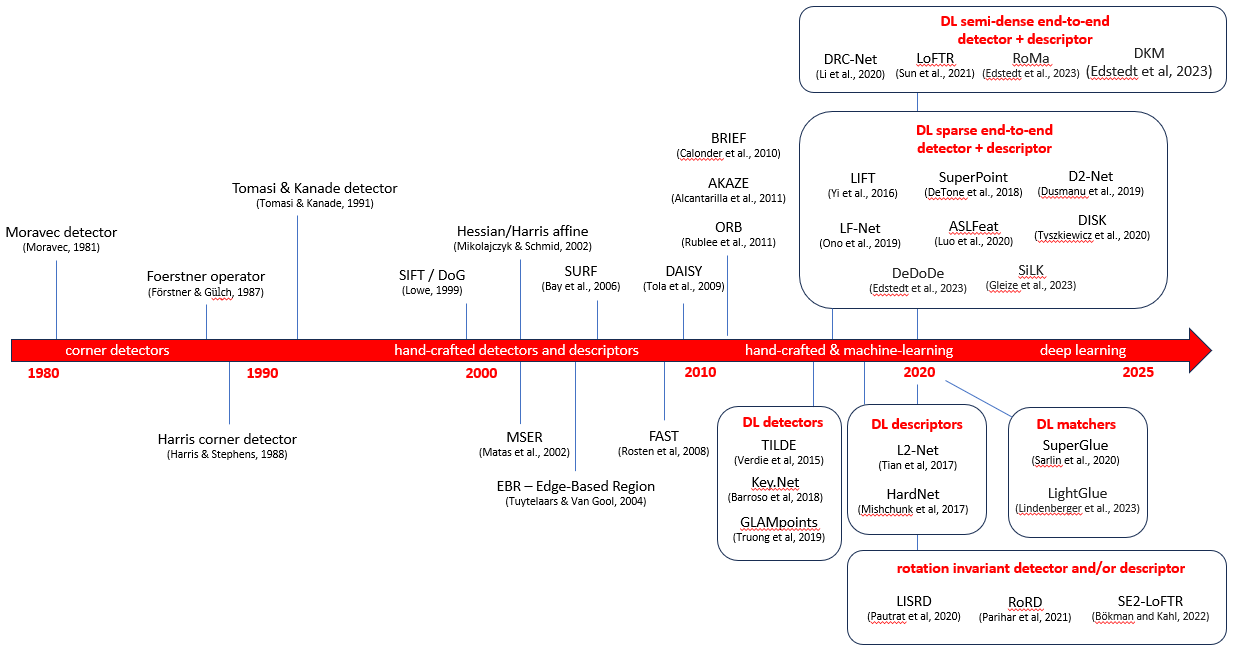
\includegraphics[width=1\textwidth]{local_feats_history}
    \caption{Timeline development of detectors, descriptors, and matches from preliminary works, hand-crafted, machine-learning, and deep-learning local features (Figure adapted from \citet{remondino2022_at_with_dl}.}
    \label{fig:4:feats_history}
\end{figure}

Historically, local image features (also known as keypoints or interest points), were initially identified manually, with automatic approaches emerging between the 1980s and the early 2000s. 
The evolution of these approaches spans a broad temporal spectrum (\figref{fig:4:feats_history}), gradually identifying algorithms that effectively deal with those fundamental characteristics necessary for reliable image features \citep{Lowe2004}. 
Image detectors should identify repeatable keypoints across different images, described by a descriptor vector that characterizes the keypoint local neighborhood allowing for similarity matching across different image views. 
These detectors and descriptors should exhibit invariance to scale differences, arbitrary rotations, radiometric changes, and multi-view perspective projections. 
Moreover, descriptors should be distinctive and unambiguous.  

Several groundbreaking works emerged, significantly contributing to the advancement of fully automatic SfM software packages. 
Particularly noteworthy is SIFT (Scale Invariant Feature Transform), which, despite its acknowledged limited invariance to illumination and affine transformations \citep{Lowe2004}, marked a significant milestone as the first detector and descriptor demonstrating sufficient invariance for a broad spectrum of applications. 
Even today, SIFT remains the benchmark feature among non-deep learning-based approaches, often referred to as hand-crafted methods \citep{jin_image_2021}. 

\figref{fig:4:feats_history} illustrates a timeline of benchmark features. 
Initially, corner detectors were utilized in the early works \citep{Harris1988ACC}, 
transitioning to blob detectors that achieved a broader degree of scale and rotation invariance \citep{Lowe2004}. 
Computational efficiency plays a pivotal role; for instance, SURF \citep{bay_surf_2006} was developed with the explicit goal of improving upon SIFT computation time, whilst ORB \citep{Rublee2011} was engineered as a binarized feature tailored for real-time applications. 

However, these methods have limitations when dealing with large camera baselines, strong viewpoint differences, and strong radiometric or scale variations \citep{Yao_2021}. 
Large camera baselines and changes in viewpoint lead to complex distortions, missing content, and occlusions between corresponding objects, making matching difficult \citep{jin_image_2021, ioli2023_replicable}.
Other challenging scenarios for traditional local features include matching historical images with contemporary datasets, e.g., for cultural heritage valorization \citep{Maiwald2021_Historical, Maiwald2023_HAI-SFM} or multitemporal aerial datasets \citep{Farella2022, Zhang2021_featmatc_histo}.

Since 2015, a novel category of DL approaches has emerged to address the limitations of existing features.
Initially, these methods involved independently training detectors and descriptors on extensive datasets comprising multi-temporal images, challenging illumination and perspective changes, and wide baselines \citep{mishchuk2018working}. % Verdie_2015
Subsequently, there has been a shift towards jointly training detectors and descriptors, starting with the seminal work of LIFT \citep{yi2016lift}, followed by other end-to-end DL approaches such as LF-Net \citep{ono2018lfnet}, SuperPoint \citep{DeTone_2018}, and ASLFeat \citep{luo2020aslfeat}.
Generally, any combination of hand-crafted and DL approaches is feasible \citep{jin_image_2021}.

Additionally, the matcher component can also be trained using DL techniques.
A pioneering and groundbreaking approach in this regard was SuperGlue \citep{sarlin2020superglue}, which makes use of an attention-based architectures~\citep{vaswani2023attention} to dramatically improve matching results by exploiting self- (intra-image) and cross- (inter-image) attention to leverage both spatial relationships of the keypoints and their visual appearance.
Superglue has been recently followed by a faster update named LightGlue \citep{lindenberger2023lightglue}. 
Recently, semi-dense matchers such as LoFTR \citep{sun2021_loftr} and RoMa \citep{edstedt2023roma} have been developed. 
However, it is noteworthy that they can identify tie points only on image pairs, as they are detector-free matchers. 
As these semi-dense matchers are not designed to build tracks of features in multiple images, they are not suitable for multi-view image orientation.

Several works have proved the effectiveness of DL approaches against varying illumination conditions, multi-temporal datasets, wide baselines, and significantly different view angles.
These challenging scenarios include glacier monitoring with wide camera baselines \citep{ioli2023_replicable, ioli2024deep}, 
multi-temporal image matching \citep{Maiwald2023_HAI-SFM}, 
multi-temporal co-registration problems \citep{Maiwald2021_Historical, Morelli2022_photogrnowandthen}, 
visual-odometry and SLAM \citep{morelli2023colmap}, 
aerial triangulation \citep{remondino2022_at_with_dl} 
and in terrestrial laser scanning point cloud registration \citep{Markiewicz2023}.
Despite these advantages, well-known limitations of DL approaches are their computational complexity, 
limited scale and rotation invariance of the descriptors, and their application on high-resolution images, 
as they have been designed for low-resolution images.

% \textcolor{red}{Add example of usage with references!}

\section{The low-cost stereoscopic system}\label{sec:4:system}

The low-cost stereoscopic system employed for short-term monitoring of the Belvedere Glacier consists of two autonomous and independent monitoring units. 
Each unit consists of a monitoring station that includes an off-the-shelf DSLR camera, a circuit for scheduling of image acquisition and controlling the system, a solar-based power supply system, and a case for protecting the system from the harsh environment. 
The core of each monitoring unit is the controlling circuit, which is composed of an Arduino microcontroller for camera triggering, and a Raspberry Pi Zero with a SIM card for sending images to a remote server via a GSM network~\figref{fig:4:scheme_foto}.
The total cost of each unit was less than \texteuro2000, including camera and lens \citep{ioli2023_replicable}.

The system was designed and built by adapting to the alpine environment an existing open-source model developed by Greig Sheridan and published on
GitHub\footnote{\label{foot:greig}Greig Sheridan' Intervalometerator repository:
  \url{https://github.com/greiginsydney/Intervalometerator}}.
A key aspect of the project was to ensure easy assembly and realization of the system to guarantee future replications and improvements.

This section describes the monitoring system and its installation at the Belvedere Glacier.

\begin{figure}[ht!]
  \centering
  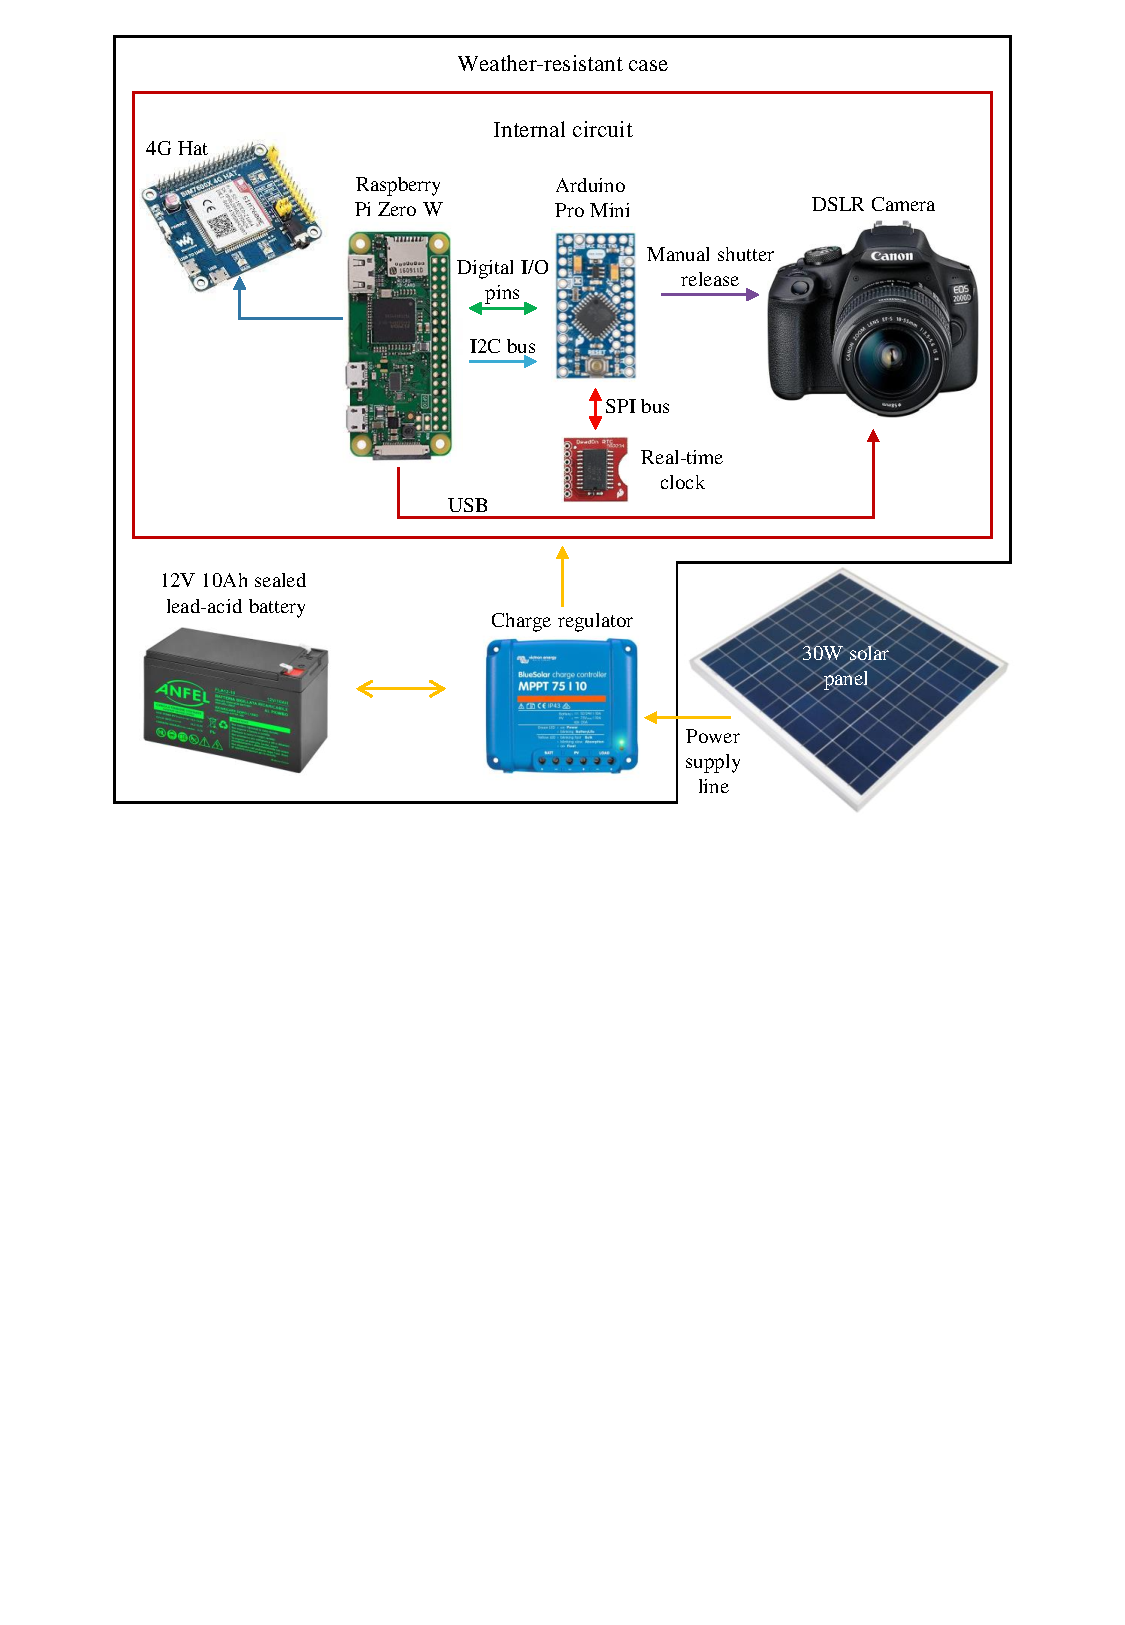
\includegraphics[width=0.6\textwidth]{schema.pdf}
  \caption{Scheme of a single monitoring station's proposed acquisition system configuration. Arrows indicate the direction of signal initiation. Image adapted
    from Greig Sheridan's repository.}
  \label{fig:4:scheme_foto}
\end{figure}


\subsection{Power supply}\label{Power_supply}
Each monitoring unit has its autonomous power supply line (yellow arrows in Figure
\ref{fig:4:scheme_foto}) provided by a solar panel combined with a sealed lead-acid
battery. An MPPT (Maximum Power Point Tracker) charge regulator directly connects with
the unit's internal circuit, providing a regular current supply to the battery
and the load and exploiting all the power generated by the panel. This regulator prevents
any excess current that may damage the connected device, thus increasing the reliability of the system. 
Its battery life-saving algorithm modulates the load disconnection level
so that a nearly 100\% recharge is achieved about once every week and, in case of battery discharging, the whole system is switched off until 100\% recharge of the battery is achieved.
The whole monitoring system is designed to minimize power consumption, e.g., by powering off devices responsible for the highest power consumption when not needed.
An estimation of the system's energy consumption guided the choice of the components of the power supply line. 
Specifically, the battery and the associated panel must be accurately dimensioned for the system's purpose. 
To this end, the Photovoltaic Geographical Information System (PVGIS)\footnote{\url{https://re.jrc.ec.europa.eu/pvg_tools/en/}}, a tool provided by the European Commission, was used.
PVGIS can estimate the performance of off-grid photovoltaic systems according to the installation site and it is supported by a database and algorithms for calculating solar radiation. 
Tuning the parameters for the Belvedere Glacier location and the system consumption, we ended up with the specifications of solar panel power of 30 W, a battery voltage of 12 V, and a capacity of 10 Ah. 
Some compromises were made, accepting that the system would not be sufficiently powered in the months with the lowest solar radiation (November, December, January, and February). 

\subsection{Controlling circuit and acquisition scheduling}\label{Control}

\begin{figure}[ht!]
  \centering
  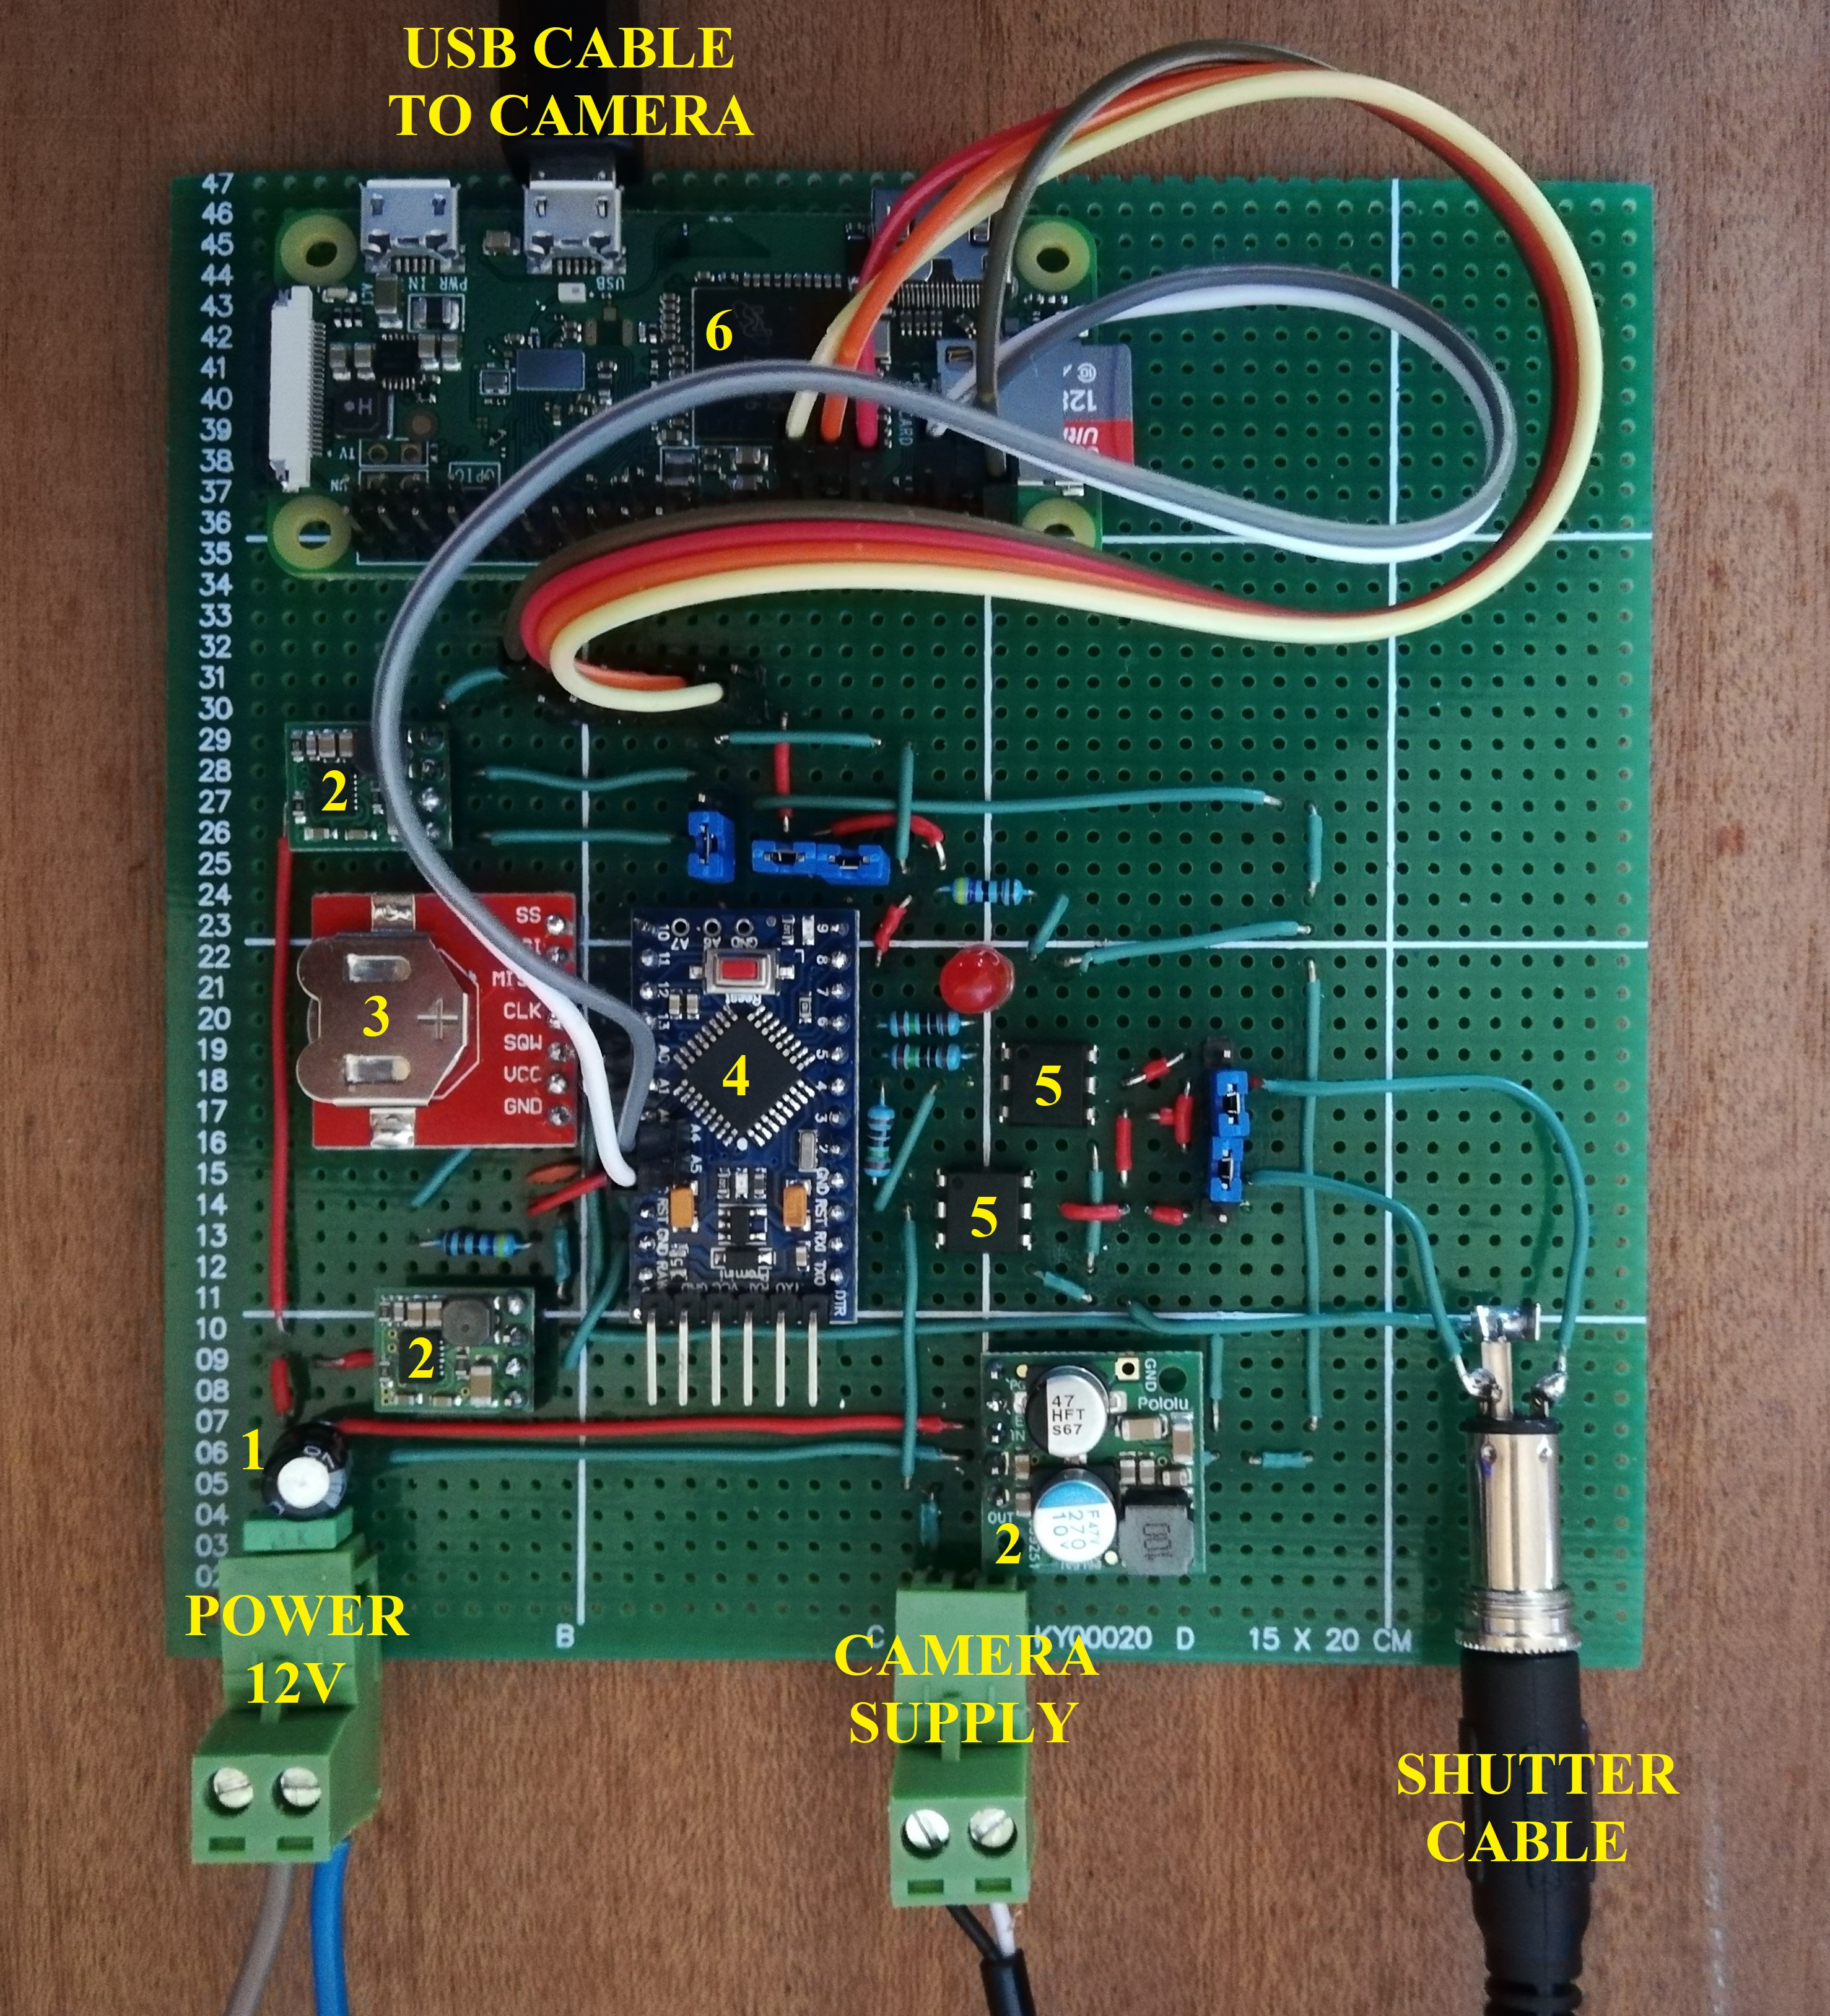
\includegraphics[width=0.6\textwidth]{board.jpg}
  \caption{Stripboard on which are soldered the main components of the internal
    circuit: capacitors (1), voltage regulators (2), real-time clock with coin-cell battery (3), Arduino Pro Mini (4), optoisolators (5), and Raspberry Pi Zero W (6). \textcolor{red}{Add pic of new board}}
  \label{fig:4:circuit}
\end{figure}

The internal electronic circuit (red box in \figref{fig:4:scheme_foto}) of the
monitoring unit is the only load connected to the power supply and is responsible for all
the system's control and scheduling functionalities.
Its components are a real-time clock (number 3 in \figref{fig:4:circuit}) with a 12
mm
coin-cell backup battery, an Arduino microcontroller (Pro  Mini 328 3.3V 8MHz, number 4
in \figref{fig:4:circuit}), a Raspberry Pi Zero W with 128 GB SD memory card (number
6 in \figref{fig:4:circuit}), and minor elements for connections, isolation (capacitors and optoisolators numbers 1 and 5 in \figref{fig:4:circuit}), and voltage regulations (numbers 2 in \figref{fig:4:circuit}).
The circuit was realized manually by soldering wires and components on a stripboard (see \figref{fig:4:circuit}).

The Arduino communicates through an SPI (Serial Peripheral Interface) bus with an
accurate real-time clock to schedule its actions: waking the camera, firing the shutter to take a photo, and turning on/off the Raspberry. 
The Raspberry can access the camera images and transfer them to a remote server via internet connectivity. 
A large storage memory is added to the unit to save photos before remote transferring. 
The Raspberry also provides a web-based, user-friendly interface
(\figref{fig:4:web-interface}) to configure and monitor the system remotely
\citep{greig}.
An I2C (Inter Integrated Circuit) bus and digital pin connections enable higher-level
communication between these two boards. Among the minor components, we mention the role
of the three voltage regulators. They allow each unit to be powered at the appropriate
voltage and current: starting from the 12 V in input, one delivers 3.3 V and 500 mA to
the Arduino, one 5 V and 2.5 A to the Raspberry and its hat, and the other 7.5 V and 2.4
A to the camera. The Arduino controls the 5V regulator of the Raspberry to reduce
quiescent power consumption when the Raspberry board is off.

Acquisition of a defined number of images, camera triggering and timing, and sending of
images to a remote server can be scheduled thanks to adequate programming of a cyclic
executive program in C++ for Arduino and of services automatically executing Python
scripts for the Raspberry.
All the monitoring station activities can be remotely scheduled from the terminal or a
user-friendly web interface \citep{greig}. 
This useful feature allows one to change the settings and check the behavior of the system, 
avoiding the need for manual intervention. 
The Raspberry uses the gPhoto2, a Python-based protocol developed to specifically interact with popular cameras’ firmware, to communicate with the camera and access new photos. 
The web-based interface service is based on NGINX and Gunicorn, open-source software for web servers. 
The interface (\figref{fig:4:web-interface}) consists of a web page accessible with credentials and provides a summary of the system state and the exact time of the last operations (time of the last shot and the last upload of images), temperatures of the components, previews of the last images, buttons to wake up the camera, take a preview photo and schedule the system routine (time and number of photo acquisition, wake-up time of the Raspberry) and some camera settings.

\begin{figure}[ht!]
  \centering
  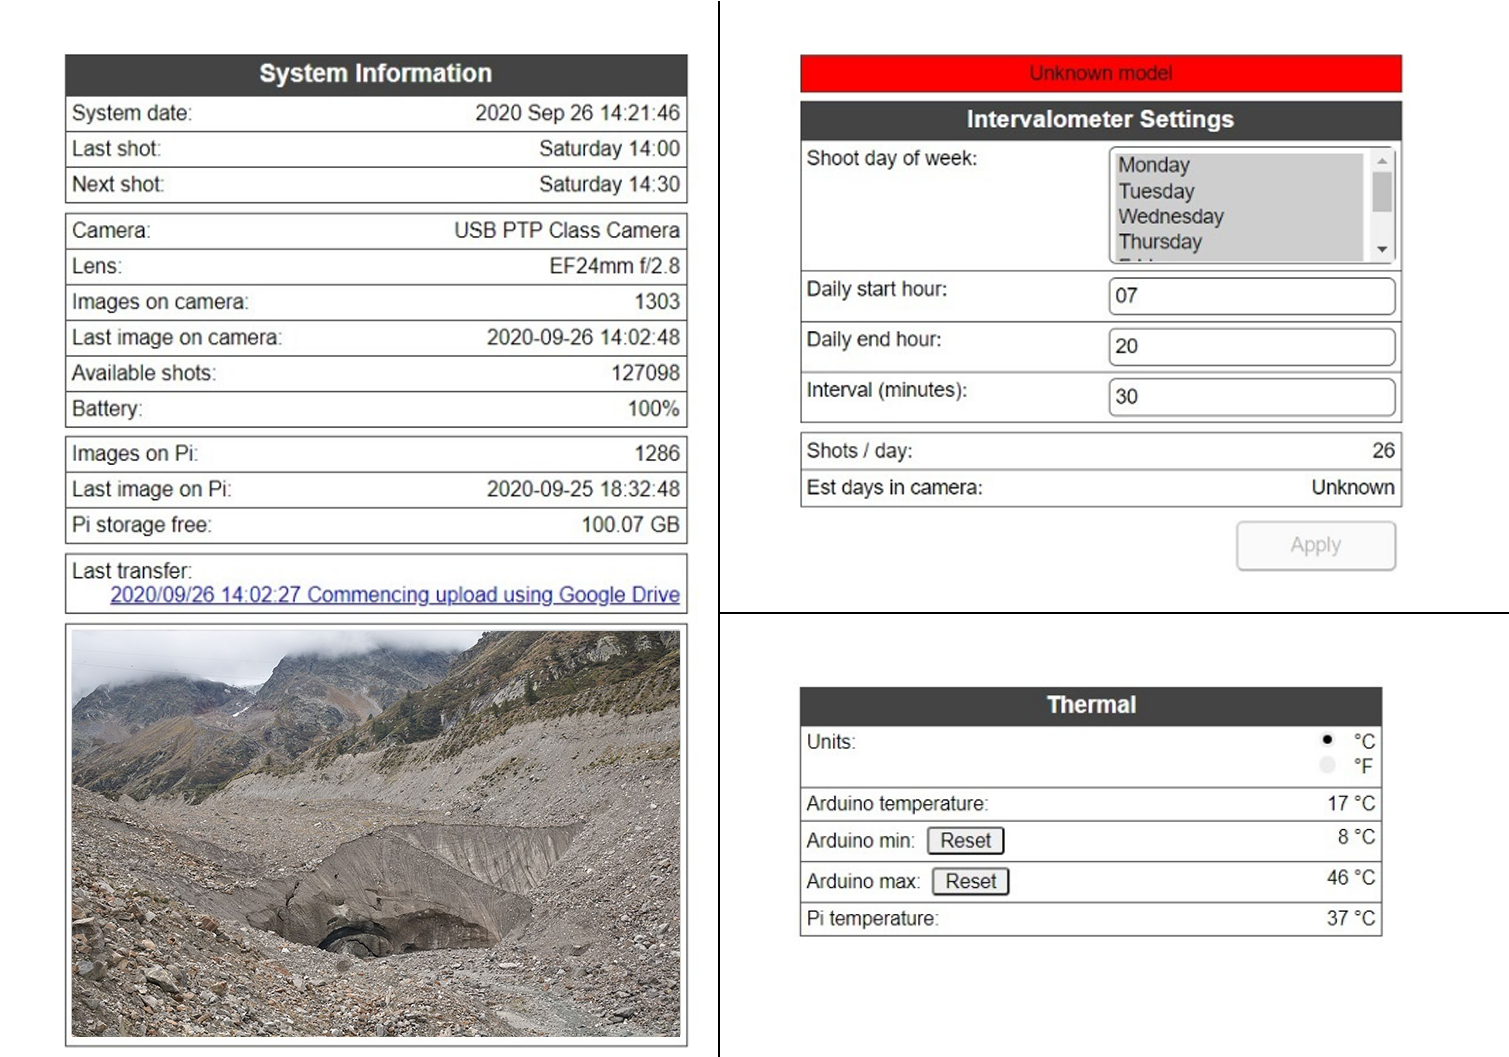
\includegraphics[width=1\textwidth]{web_interface.png}
  \caption{Example of some of the pages of the web-based interface to remotely control
    the monitoring units.}
  \label{fig:4:web-interface}
\end{figure}

All the components were chosen because of their low power consumption and their
inter-compatibility. 
The circuit is robust against power losses due to battery discharging and can auto-recover when power is regained. 
A low energy consumption policy is also followed in selecting the scheduling. 
The camera is switched on only during the data capture activity. 
The Raspberry is switched on only once per day when the connection with the remote server and image transfer is scheduled.

\subsection{Connectivity}\label{Connectivity}
Internet connectivity is crucial to transfer images and to control the units remotely. To
this end, the Raspberry is equipped with the SIM7600E-H 4G hat by Waveshare. The module
supports 4G/3G/2G communication via a SIM card. Raspberry and hat operations are the most
expensive in terms of power consumption. For this reason, the board is switched on only
once a day for a limited period, which is kept adequately low to be sustainable
for the system power supply but still sufficient for transferring new images to the
server. We adopted IoT (Internet of Things) SIM cards provided by the multi-operator
service Emnify \citep{emnify}, as it offers the ability to connect to the best-quality
cellular network available and includes flexible and customizable data plans.
Remote access to the devices is allowed by a VPN (Virtual Private Network).
The service costs \texteuro33 per month for a data plan with 6 GB.

\subsection{Case and protection}\label{Case and protection}
The majority of the components need to be protected. Therefore, a solid and compact case
that allows keeping all the parts (except the solar panel) in the same
location is desirable for the functioning of the system and convenient
transportation, installation and maintenance. The case should also satisfy the thermal
insulation requirements according to each component's working temperature range. The case
should also be waterproof and robust against different and harsh weather conditions but,
at the same time, provide access for connecting the solar panel and taking pictures. Our
choice was an HPRC 2250 lightweight, waterproof resin case with internal insulating foam.
The foam was found to be useful in enhancing the temperature seal and stabilising the
location of some components, preventing unwanted movements. Holes were drilled in the
case: one sealed with a UV filter of 82 mm to allow the camera to take shots, two others
to give access to the solar panel wires, and others to fix the system to a tripod. The
internal case dimensions (236x182x155 mm) posed a significant challenge in accommodating
all the components inside. In particular, the camera lens dimensions were constrained by
space availability.

\subsection{General performances}\label{General_performances}
The system was subject to several tests before being used in its final application at the
Belvedere glacier site. During these tests, the system proved to be autonomous, robust to
sudden shutdowns, cold-resistant, water-resistant, and self-sufficient for a prolonged
period with no direct sunlight on the solar panels. 
Specifically, in the absence of sunlight, the battery can power the system for about nine days before it is completely discharged. 
Battery voltage and temperatures of components were monitored, simulating the absence of solar radiation and low environmental temperatures.
Figure \ref{fig:4:nominal_performance} shows the performances of the system during these tests.

\begin{figure}[ht!]
  \centering
  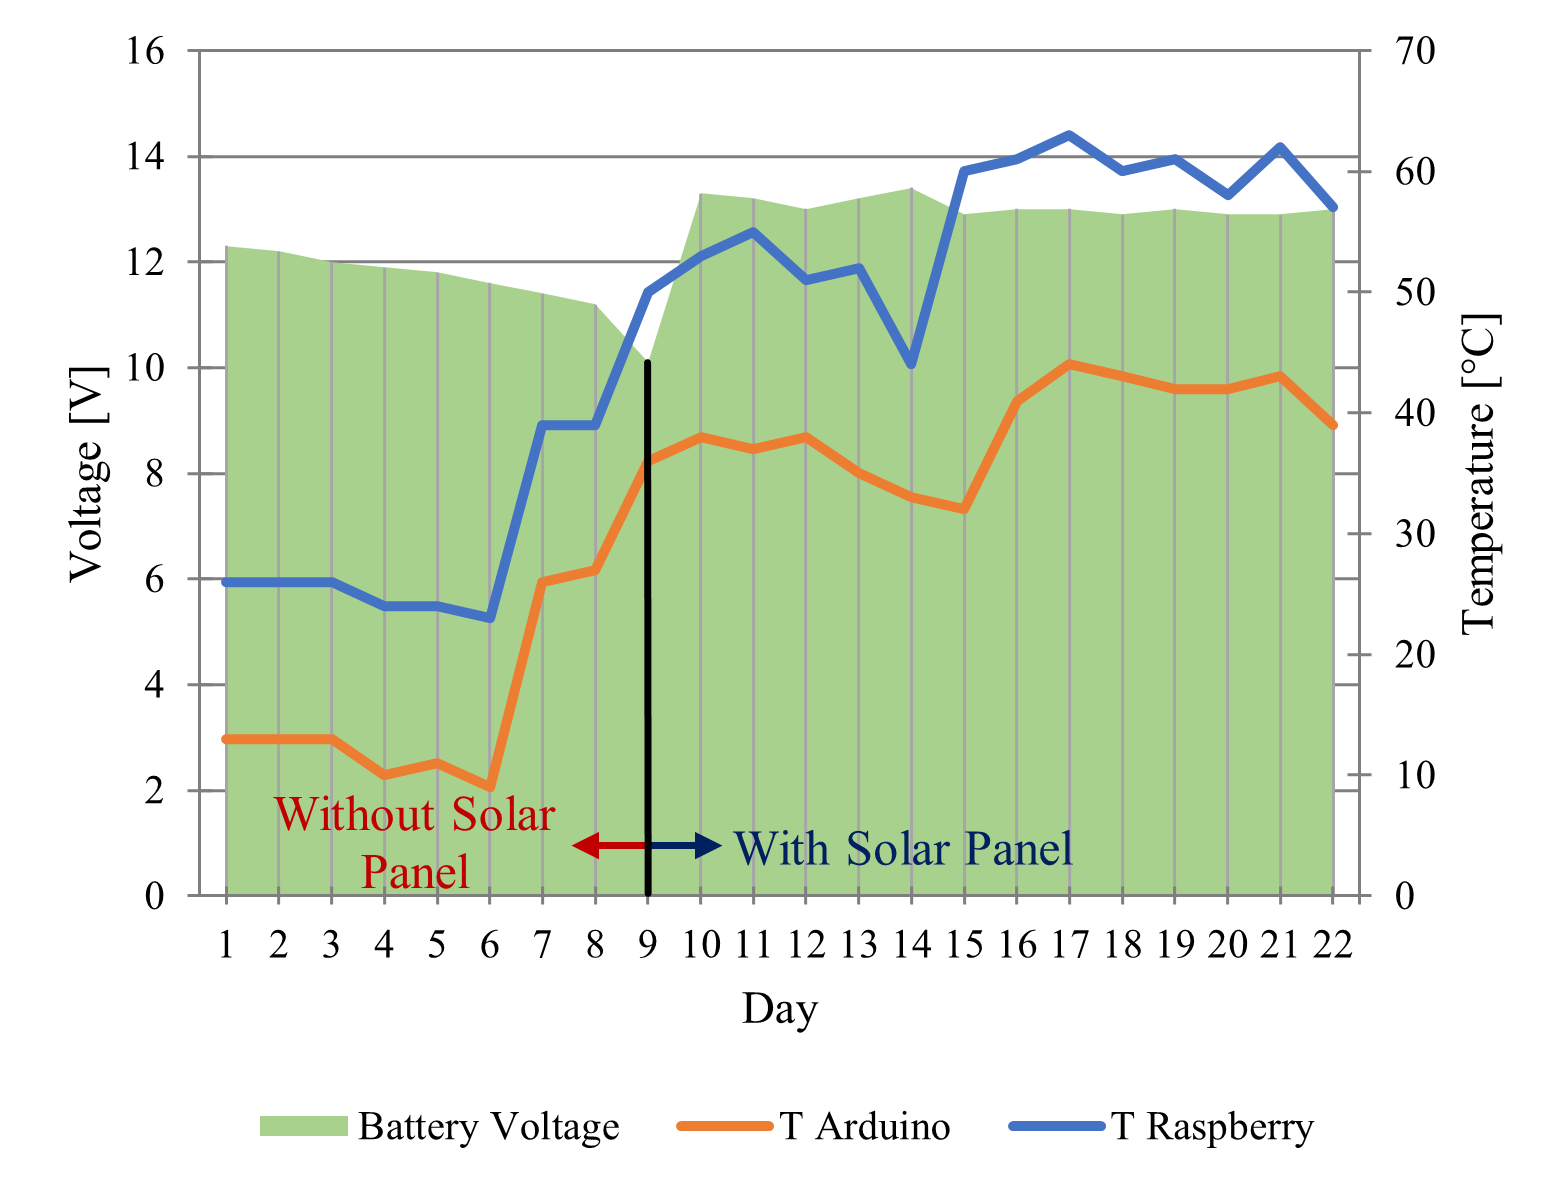
\includegraphics[width=.6\textwidth]{nominal.png}
  \caption{Battery voltage and temperature of boards with and without the solar panel
    during a period of tests. Starting from a fully charged condition, the system was
    kept without solar panel at around 2 °C for the first six days. After nine days, the
    battery was fully discharged and the system was reconnected to the panel and exposed
    to solar radiation.}
  \label{fig:4:nominal_performance}
\end{figure}

\subsection{The choice of the camera}\label{camera}
The choice of the DSLR camera and the optics can be considered application-dependent.
Therefore specifications regarding these components are reported referring to the
Belvedere glacier case study. 
Each monitoring station was equipped with a DSLR camera Canon EOS 2000D, with 24.1 MP CMOS \mbox{APS-C} sensor. 
This model was chosen because of the limited costs, the high image resolution, and its compactness, as it must fit inside the case. 
Additionally, another fundamental requirement was camera compatibility with the \textit{gPhoto2} software. 
The choice of the lenses is mostly site-specific, as it is driven by the required GSD of the images, in addition
to dimensional constraints that limit the choices of the optics to rather small lenses that can fit into the protective case.
The lenses chosen for the two cameras are described in \secref{sec:4:siteselection}.

In the installation inside the system case, the traditional rechargeable battery was replaced by a special battery 
(”fake battery”) equipped with a power supply cable, which provides a voltage of 7.5 V from the circuit. 
The camera is attached to a sliding plate able to vary, with a limited range, and then fix the position of the camera 
on the longitudinal axis. Screws fix the camera to the plate and the plate to the case.

\subsection{Site selection for permanent installation}\label{sec:4:siteselection}

A preliminary survey was conducted to identify suitable locations for the two monitoring units. 
The primary goal was to ensure both cameras had a clear view of the northwest terminal lobe, particularly the terminal ice cliff,
as this area experiences substantial transformation and retreat. 
However, the harsh glacial environment presented significant challenges. 
The glacier's steep moraines are mostly unstable due to reduced support from the melting ice, making them prone to sliding and collapsing.

Another critical consideration for a good acquisition geometry is the baseline (i.e., the distance between cameras). 
This distance should be sufficiently large relative to the camera-object distance to avoid compromising depth estimation accuracy due to narrow perspective ray intersection. 
Consequently, installing the cameras close together on the same side of the glacier was not feasible.

\begin{figure}
  \centering
  \subcaptionbox{\label{fig:4:studyarea:map}}{
    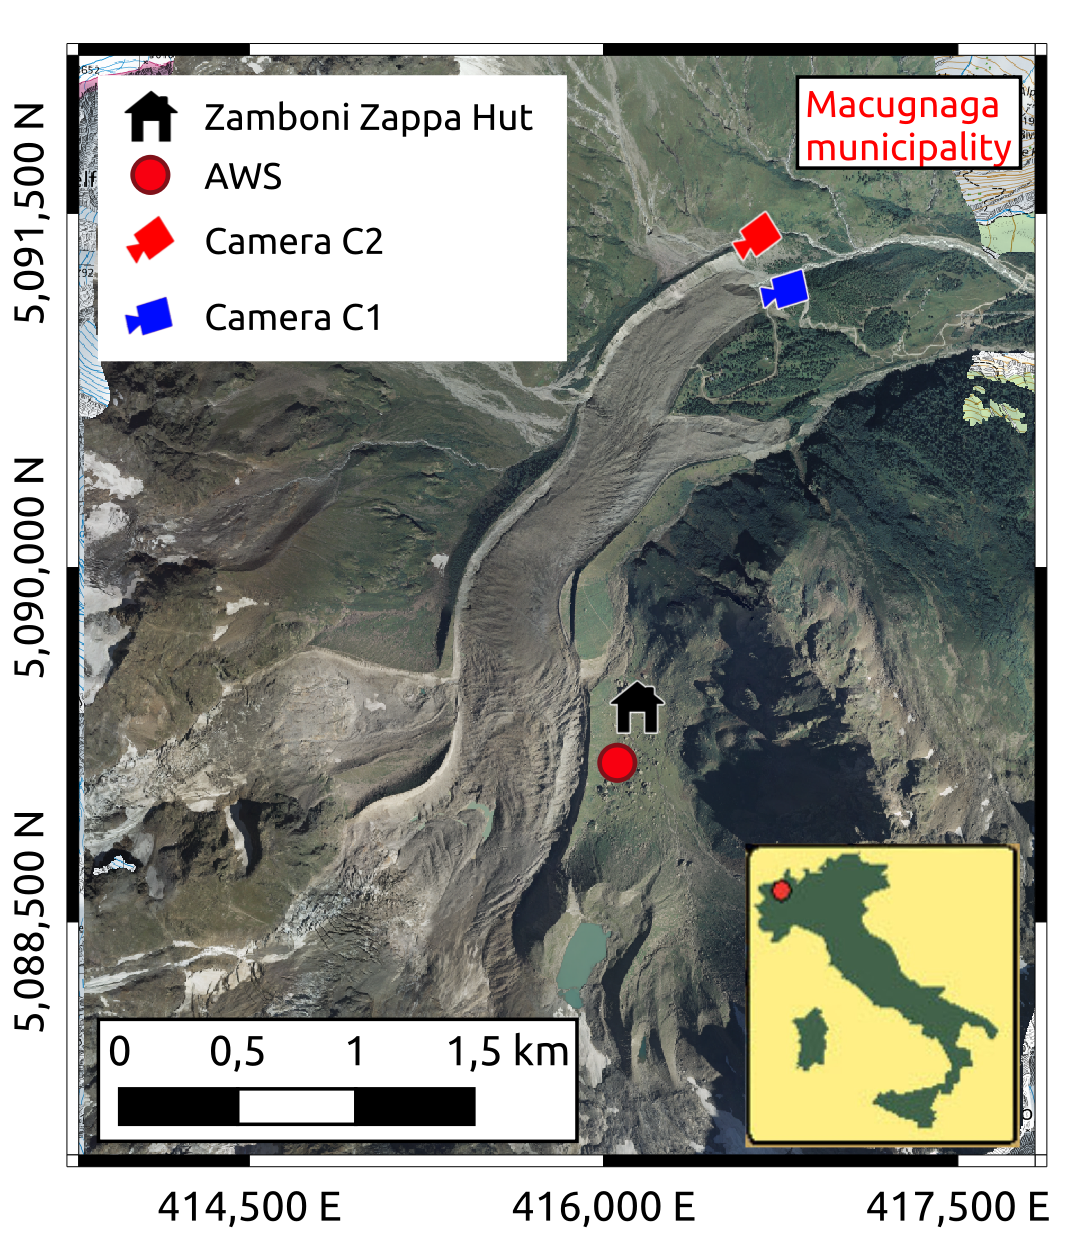
\includegraphics[width=.3\textwidth]{2_geographic_framework.png}
  }
  \subcaptionbox{\label{fig:4:studyarea:pic}}{
    \includegraphics[width=0.67\textwidth]{2_area_of_sudy.png}
  }
  \caption{(a) Map of the Belvedere Glacier, with marked the location of the two cameras C1 and C2, the Automatic Weather Station (AWS) and the Zamboni Zappa Hut;
  (b) The area of study: the stereoscopic reconstruction is focused on the terminal ice cliff (dashed light blue line), while the monoscopic DIC processing from camera C2 image sequence is focused on the upper area of the north lobe (dashed green line).}
  \label{fig:4:studyarea}
\end{figure}

Ultimately, two large boulders located on opposite moraines flanking the glacier's terminal lobe were identified as the only suitable and stable locations\figref{fig:4:studyarea}.
The cameras, labelled as C1 and C2, were installed in July 2021 approximately at \SI{\sim230}{\meter} and \SI{\sim350}{\meter} from the terminal ice cliff respectively, with a strongly convergent pose~\figref{fig:4:studyarea}.

To ensure comparable Ground Sample Distance (GSD) of the images (\SI{\sim 3.5}{\centi\meter\per\pixel}), lenses with different focal lengths were employed. 
A Canon EF 24 mm f/2.8 IS USM was used for camera C1 (stream-wise right) and a Canon EF 35 mm f/2 IS USM was used for camera C2 (stream-wise left).
A summary of the characteristics of the cameras and lenses employed is provided in \tabref{tab:4:cameras}.

\begin{table}
  \centering
  \caption{Summary of the characteristics of the two cameras.
    Fields marked with $^*$ are computed considering the distance between each camera and
    the ice cliff.}
  \label{tab:4:cameras}
  \begin{tabular}{c c c}
    {}              & C1                               & C2 \\
    \hline\noalign{\smallskip}
    Camera          & Canon Eos 1200D
                    & Canon Eos 1200D                       \\
    Sensor          & APS-C
                    & APS-C                                 \\
    Pixel size      & \SI{3.7}{\micro\meter}
                    & \SI{3.7}{\micro\meter}                \\
    Image           & \qtyproduct{6000x4000}{\pixel}
                    & \qtyproduct{6000x4000}{\pixel}        \\
    Lens            & Canon EF 24mm f/2.8 IS USM
                    & Canon EF 35mm f/2 IS USM              \\
    Distance$^*$    & \SI{230}{\meter}
                    & \SI{350}{\meter}                      \\
    Average GSD$^*$ & \SI{3.5}{\centi\meter\per\pixel}
                    & \SI{3.5}{\centi\meter\per\pixel}      \\
    \noalign{\smallskip}\hline
  \end{tabular}
\end{table}

The baseline between the two cameras of \SI{\sim 261}{\meter} ensured a good
viewing geometry because of the large parallax between corresponding points.
However, the baseline comparable to the camera-object distance (base-height ratio close
to \(1\), \tabref{tab:4:cameras}) led to complex affinity-like distortions and occlusions
between corresponding areas in the two images~\citep{Yao_2021}.
Additionally, C1 was positioned at a lower viewpoint compared to C2, due to
site geometry constraints.
Therefore, camera C1 provides a limited view that primarily encompasses the frontal ice
cliff, but does not capture the glacier surface, which is only visible from camera C2.


\subsection{Camera monumentation}\label{sec:4:cameramonumentation}
The cameras were mounted on large, stable rocks along the moraines using aluminum topographic tripods anchored with steel dowels and cables (\figref{fig:4:final_installation}). 
A central steel tie rod secures each system. 
This agile monumentation approach allows for relatively easy on-site assembly and disassembly within the challenging environment, minimizing cost and time requirements. 
The equipment was transported to the site via backpacks, often traversing unmarked terrain.

Despite these efforts, analysis of the acquired images revealed minor instability in both cameras, particularly small rotations around the vertical axis and wind-induced vibrations. While achieving perfect stability in a mountain environment is challenging, the use of GCPs located in stable areas will enable the estimation of camera orientation during image processing.

\begin{figure}[ht!]
  \centering
  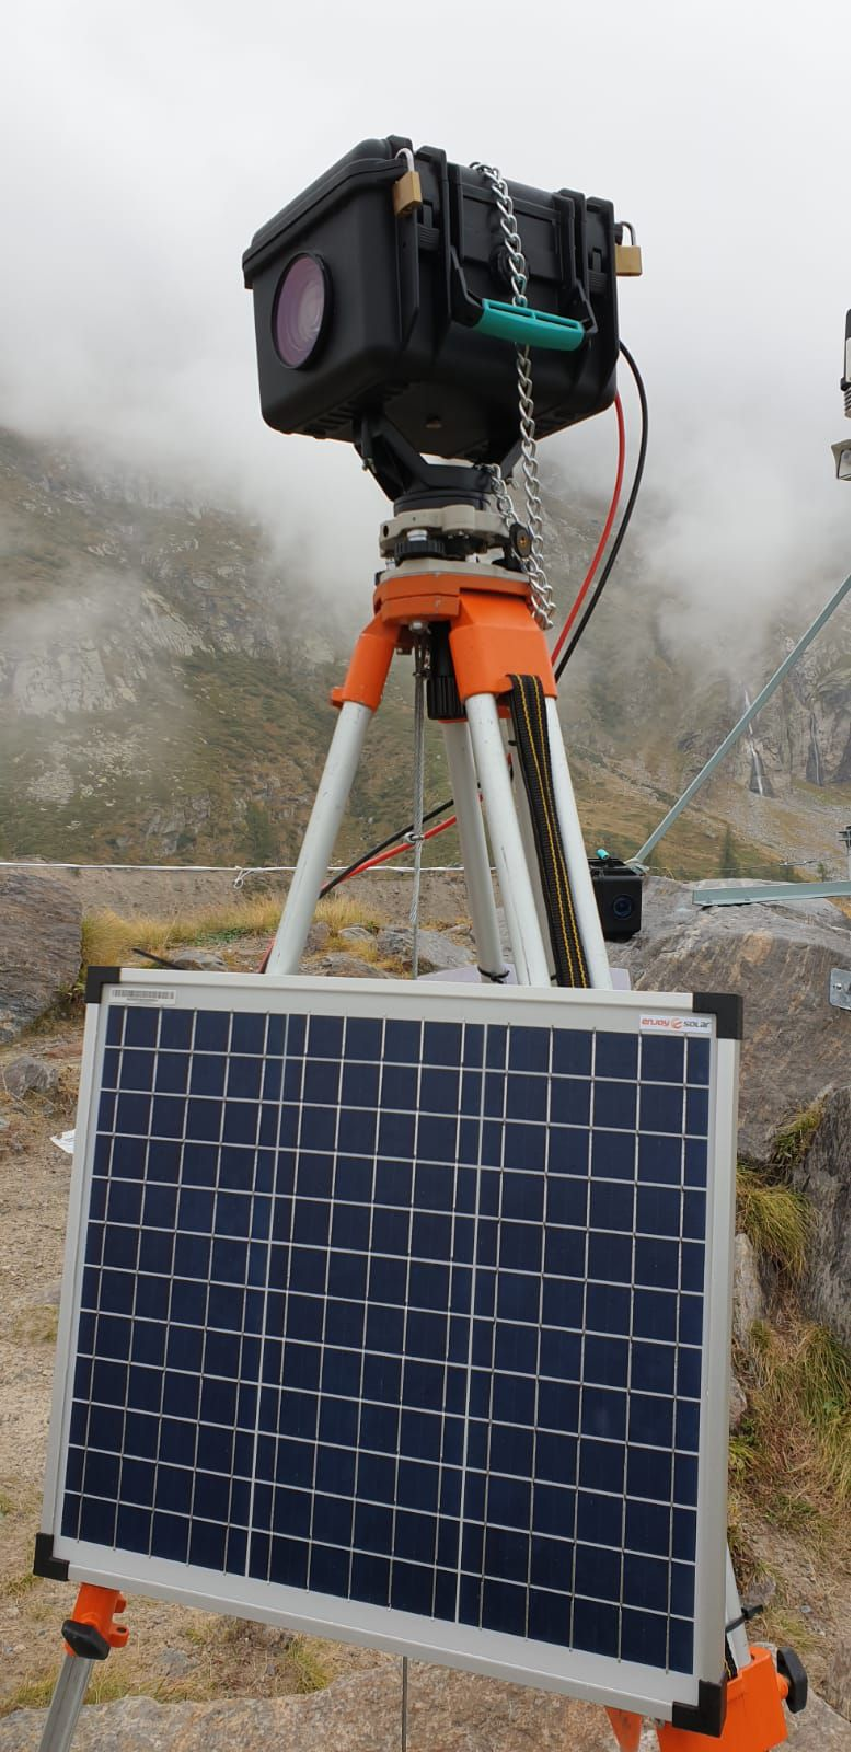
\includegraphics[width=.2\columnwidth]{finale1.pdf}
  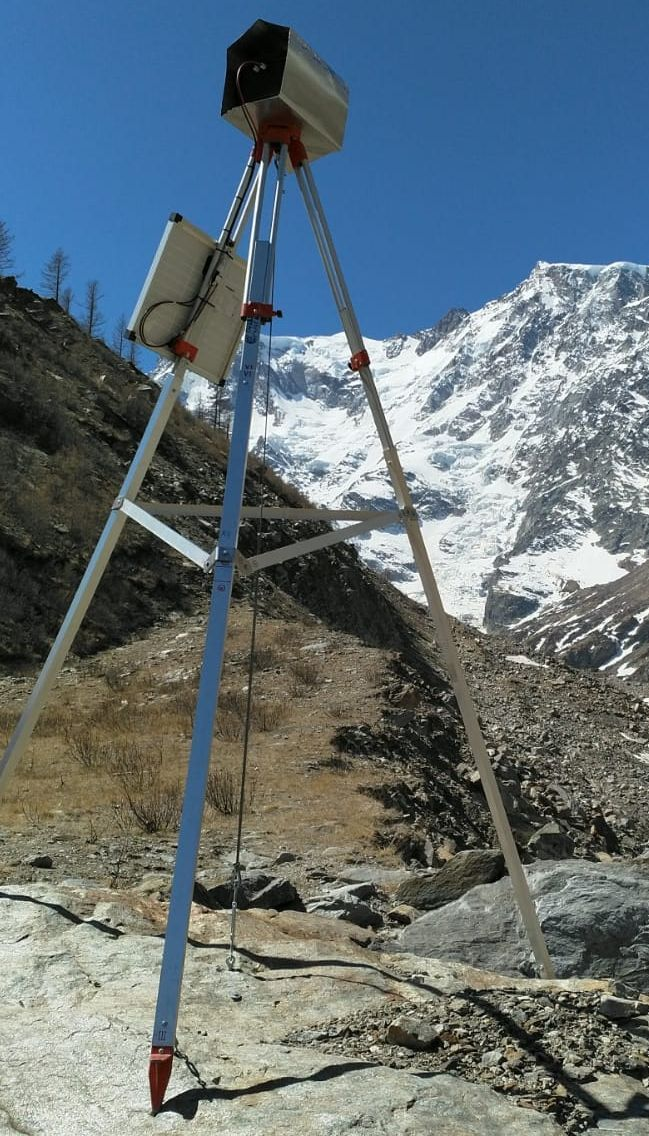
\includegraphics[width=0.3\columnwidth]{centralina.jpg} \\
  \centering{(a)\hspace{30mm}(b)}\\ \vspace{1mm}
  \caption{(a) Picture of the monitoring unit prototype installed for tests at the
    Belvedere Glacier site. (b) Picture of the final monumentation of the camera
    installed on the stream-wise right moraine.}
  \label{fig:4:final_installation}
\end{figure}

% Monumentation of the two cameras at the Belvedere Glacier site was achieved by choosing
% two large stable rocks along the moraines.
% Each camera is supported by an aluminium topographic tripod system anchored with steel
% dowels and cables to the rocks (\figref{fig:4:final_installation}b).
% A central steel tie rod keeps the system in a fixed position.
% The choice of an agile monumentation was aimed at having a system that can be rather
% easily assembled on site (and also disassembled, if needed), also in a harsh environment,
% with limited costs and time.
% To install the cameras, in fact, all the equipment was carried in backpacks along the
% moraines, sometimes without a marked walking path (e.g., in the case of the stream-wise
% left camera).
% As a drawback, the analysis of the acquired photos revealed a non-optimal stabilization
% of the two cameras.
% In fact, small rotations, especially around the vertical axis, and vibrations, mostly
% induced by the wind, were experienced.
% Though, a perfectly stable monumentation in a mountain environment is hardly achievable.
% Therefore, it is not possible to assume the camera orientation as stable a priori, but
% camera orientation must be estimated based on some Ground Control Points (GCPs) located
% on the ground in stable areas.


% The baseline between the two cameras of \SI{\sim 261}{\meter} ensured a good
% viewing geometry because of the large parallax between corresponding points.
% However, the baseline comparable to the camera-object distance (base-height ratio close
% to \(1\), \tabref{tab:4:cameras}) led to complex affinity-like distortions and occlusions
% between corresponding areas in the two images~\citep{Yao_2021}.
% Additionally, C1 was positioned at a lower viewpoint compared to C2, due to
% site geometry constraints.
% Therefore, camera C1 provides a limited view that primarily encompasses the frontal ice
% cliff, but does not capture the glacier surface, which is only visible from camera C2.

\subsection{System operation and cost-effectiveness}

The stereoscopic system was operating from August 2021 up to December 2022, when it was
temporarily unmounted for ordinary maintenance, and finally mounted again in June 2023.
During the operational period, the system was programmed to acquire two images per day,
but only one image per day was used for the multitemporal processing.
Only daily images taken during the snow-free period between 01/05/2022 and
13/11/2022 were considered.
In this period, the glacier experienced the most significant changes, flow velocity
and ablation rates. On the other hand, during winter and spring seasons, the glacier was
covered by snow, making it difficult to extract relevant information from optical images
for tasks such as 3D reconstruction and surface velocity estimation.

It is worth mentioning the performances of the system in terms of costs: our  monitoring
system can be fully reproduced with an average cost of \texteuro2000 per station
(November 2023), including camera (\texteuro400), lens (\texteuro500) and material for
the on-site installation (\texteuro150).
In comparison, commercial time-lapse cameras are expensive
(e.g., PhotoSentinel\footnote{PhotoSentinel: \url{https://photosentinel.com/} (accessed
  on 15/11/23)} cameras cost more than \$ 5,000.00) and hardly customizable.
The final prototype of the monitoring station is shown in Figure
\ref{fig:4:final_installation}.

\section{Datasets}\label{sec:4:datasets}

\subsection{Stereoscopic image sequences}\label{sec:4:stereo}

During the snow-free study period (from 1/05/2022 to 13/11/2022), both camera C1 and
camera C2 were able to acquire images every day, for a total of 197 images. However, 39
images were discarded due to bad weather conditions, such as rain, low clouds, or fog,
resulting in 158 days with valid data for stereo and monoscopic processing.

\subsection{UAV surveys}\label{sec:4:uavsurveys}

Two UAV flights, spaced by a 10-days interval, were conducted in summer 2022 to acquire
ground truth data for assessing the proposed methodology.
The first UAV flight, labelled as UAV-A, was carried out on 28/07/2022 with a DJI
Matrice 300 RTK quadcopter and a DJI Zenmuse P1 camera with a 35 mm lens.
During the survey, 436 images were captured, encompassing both nadiral and oblique
perspectives.
Additionally, 19 Ground Control Points (GCPs) were measured using a combination of a
total station and Differential GPS (DGPS), employing a topographic-grade
GNSS receiver.
The GCPs included both artificial targets and natural features.
During the flight, the UAV was equipped with an on-board RTK GNSS receiver, enabling the
acquisition of camera projection centers with decimetric accuracy.
The photogrammetric block (\figref{fig:4:uavblocks}a) was processed with the commercial
software package Agisoft Metashape \citep{agisoft} by using 14 GCPs and 5 Check Points
(CPs) to evaluate the block accuracy.
The global RMSE evaluated on the CPs was equal to 4.0 cm.

The secondo UAV flight, UAV-B, was carried out on 05/08/2022 with a DJI Phantom
4 RTK, focusing on a smaller portion of the northern lobe of the Belvedere Glacier.
However, due to technical constraints, \textit{moving} GCPs located inside the
glacier body were not measured again.
Therefore, only the fixed targets located outside the glacier were employed.
Among these, 8 targets were designated as GCPs, while the remaining 4 were used as CPs.
The photogrammetric block encompassed 428 nadiral and oblique images, which
were processed using Agisoft Metashape (\figref{fig:4:uavblocks}b).
A global RMSE of 7.5 cm was obtained on the 4 CPs.

\begin{figure}
  \centering
  \subcaptionbox{\label{fig:4:uavblocks:A}}{
    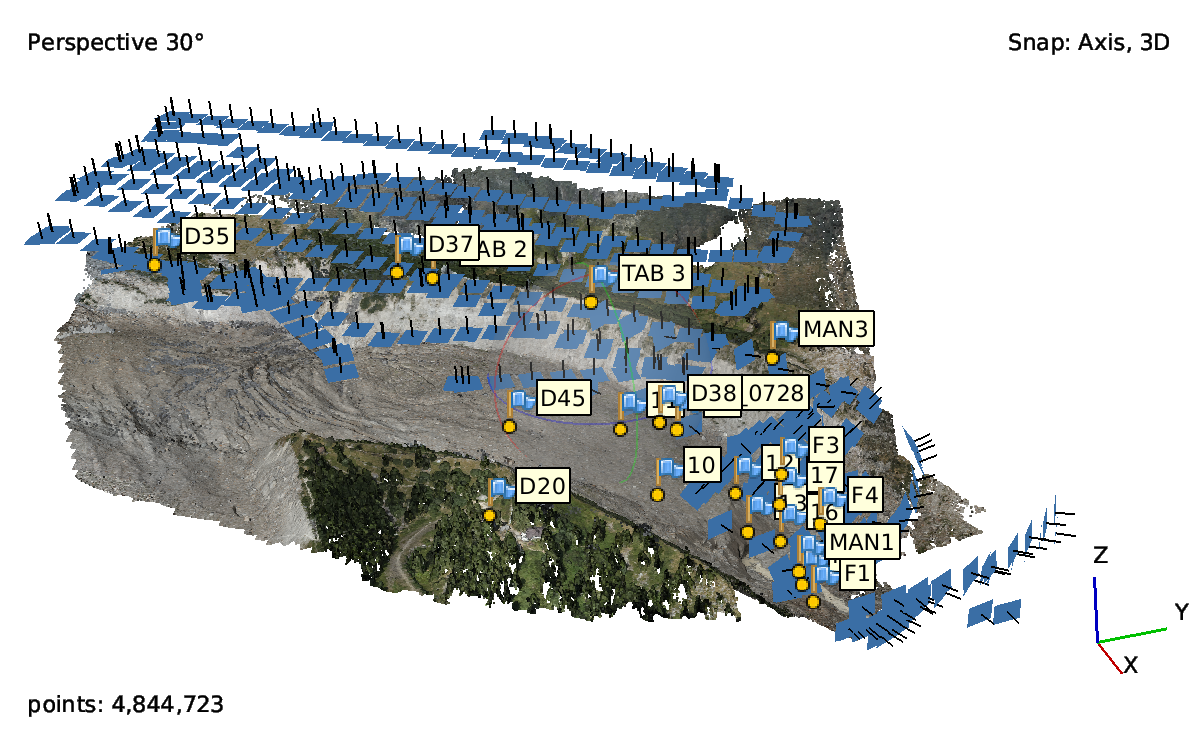
\includegraphics[width=.45\textwidth]{2_UAV-A_280722.png}
  }
  \subcaptionbox{\label{fig:4:uavblocks:B}}{
    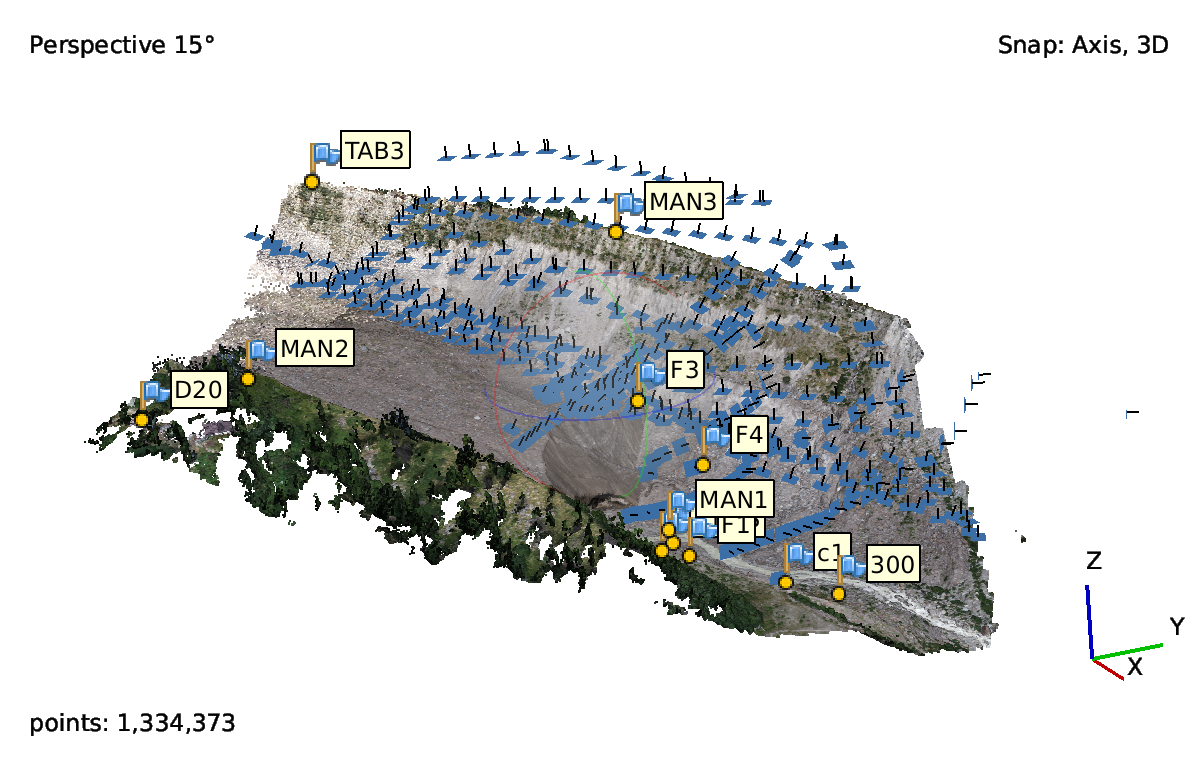
\includegraphics[width=.45\textwidth]{2_UAV-B_050822.png}
  }
  \caption{(a) UAV-A block and (b) UAV-B block processed with Agisoft Metashape. The
    flags represent the targets used either as GCPs in the BA or as CPs to evaluate the
    quality of the photogrammetric block.}
  \label{fig:4:uavblocks}
\end{figure}

\subsection{Meteorological monitoring station}\label{sec:4:meteostation}

To analyze the correlation between the Belvedere Glacier dynamics and
external environmental variables, data measured from an Automatic Weather Station (AWS)
located close to the Zamboni Zappa Hut were used.
The AWS is located at an altitude of \SI{2075}{\masl} and at a distance of
2 km from the area of study.
The data from the AWS can be downloaded from the Arpa Piemonte
website\footnote{\url{https://www.arpa.piemonte.it/rischi_naturali/snippets_arpa_graphs/dati_giornalieri_meteo/?statid=PIE-003086-906-2007-07-05&param=T}}.
In our study, we analyzed mean daily values of air temperature, precipitation and
incoming solar radiation from 01/05/22 to 15/11/22.


\section{Methodology}\label{sec:4:methodology}
This chapter outlines the methodology developed to monitor the evolution of the Belvedere
Glacier northern lobe.
The daily images were processed using a framework consisting of two parallel processing
chains (\figref{fig:4:workflow}):
(i) a photogrammetric-based stereoscopic approach;
(ii) a DIC-based monoscopic approach.
The daily stereo pairs were used to generate 3D models of the glacier terminus,
enabling the estimation of ice volume loss on a daily basis by computing point cloud
differences along the main flow direction.
However, due to limited overlapping views of the two cameras, the stereoscopic approach
primarily provides a 3D reconstruction of the terminal ice cliff (dashed-blue area in
\figref{fig:4:studyarea}b).
Consequently, deriving the 3D surface velocity field of the glacier solely from
photogrammetry was not feasible.
The image sequence captured by camera C2, offering a higher viewpoint and broader
coverage of the glacier surface, was employed to determine the glacier's surface velocity
over a larger area of the north lobe of the Belvedere Glacier (dashed-green area in
\figref{fig:4:studyarea}b).

\begin{figure*}[ht]
  \centering
  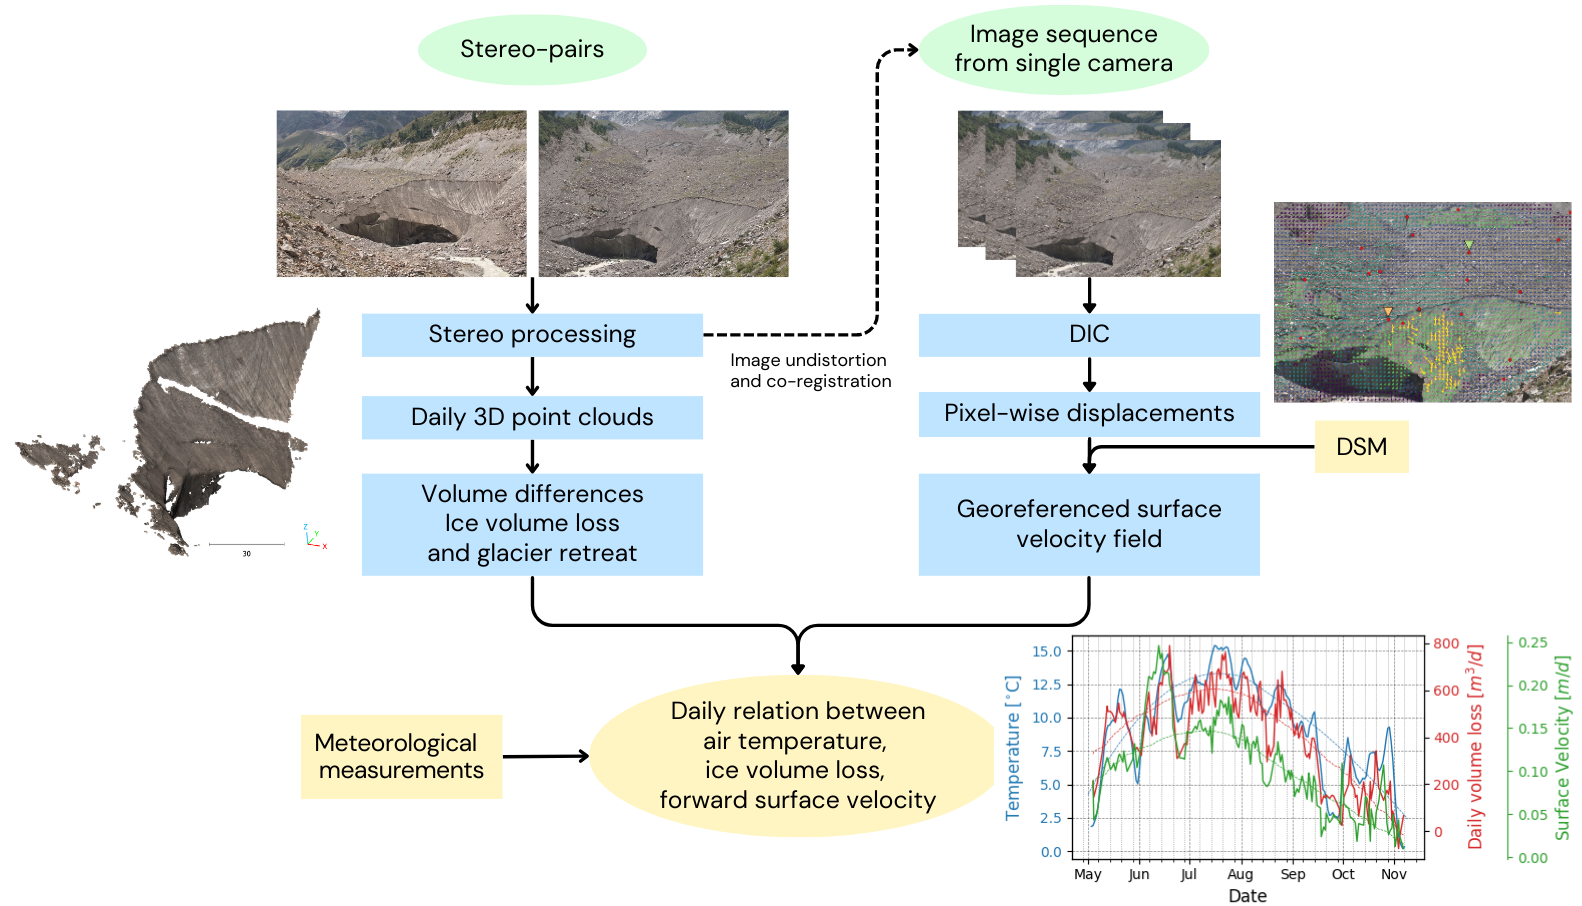
\includegraphics[width=\textwidth]{3_general_workflow.png}
  \caption{General workflow with two parallel processing chains involving stereoscopic
    reconstruction of terminal ice cliff from stereo-pairs of images to derive ice volume
    losses at the glacier terminus and glacier retreat and monoscopic digital-image
    correlation to derive surface velocities.}
  \label{fig:4:workflow}
\end{figure*}

\subsection{Image selection}\label{sec:4:imageselection}

Once the acquired images have been received from the monitoring system, an
automatic selection of the images was performed to exclude the ones acquired in rainy,
foggy, or poor lighting conditions.
This selection was based on the analysis of images median
entropy~\citep{tsai2008entropy}:
the images with a low value over the entire image were rejected.
Additionally, a visual inspection was performed on the entire image dataset.
The inspection had the following objectives:
(i) selecting only one image per day;
(ii) rejecting poor quality images that were not automatically rejected,
and images in which the fixed targets placed along the moraines were not visible;
(iii) detecting of sudden changes in the morphology of the glacier
terminus (e.g., icefall).

\subsection{Camera calibration}\label{sec:4:cameracalibration}

Each camera was mounted with all its electronics inside a waterproof case and protected
by a neutral filter that was glued to the case and fixed in front of the cameras.
Since the filter introduced additional distortion, the cameras need to be calibrated
inside the boxes to reproduce the final setup.
Therefore, a two-step approach was taken: first, a 120 cm x 70 cm calibration board with
a checkerboard printed on it was used to estimate an initial set of parameters for the
interior orientation \citep{zhang_flexible_2000}.
To this end, the cameras were mounted on tripods inside their cases while the calibration
board was moved and rotated in front of the camera to simulate a convergent hemispheric
acquisition.
For each camera, about 30 images were collected and processed in Agisoft Metashape to
obtain a first estimate of the interior orientation.
However, the average camera-to-panel distance was much smaller than the actual
camera-to-glacier distance.
Therefore, a refinement of the calibration was performed in-situ by incorporating the
stereo pair acquired by the cameras on 28/07/22, within the UAV-A block, carried out on
the same day.
This block was processed with Agisoft Metashape to refine the interior camera
orientation of the stereo cameras, aided by the increased robustness of the block given
by the additional matches between the two images taken by camera C1 and C2 and the UAV.

An additional challenge was represented by camera interior orientation stability over
time.
From experimental evidence, the interior orientation parameter that suffered the most
because of temperature variations that occurred in mountain environment
was the camera principal distance \citep{Elias2020}, while the other parameters
remained more stable during time.
To mitigate the impact of temperature-induced variations, it was crucial to incorporate
camera self-calibration during the stereoscopic processing at each epoch to refine the
pre-calibrated principal distance.

\subsection{Camera stability and GCPs}\label{sec:4:stability}

Since the two cameras were mounted on topographic tripods, the stability of the cameras
was not perfectly guaranteed. In particular, the two cameras experienced small vibrations
around their pivots due to wind gusts.
On the other hand, the position of the cameras was constrained by topographic heads that
kept the position of the camera center constant to the centimeter level.
Therefore, the baseline of the cameras can be reasonably considered as constant, with a
value of \SI{261.55}{\meter}.
On the other hand, camera angular vibrations implied that the relative orientation of the
cameras must be estimated at each epoch.
Moreover, to fix the world reference system over time, absolute orientation of the
stereo model was required.
To this end, the position of the cameras was measured in-situ using a topography-grade
GNSS receiver in RTK.
In addition, four GCPs were materialized with plastic targets, anchored to stable rocks
in front of the terminal ice cliff and along the streamwise left
moraine (\figref{fig:4:studyarea}a).
While the minimum requirement to estimate a Helmert transformation would have been just
the two cameras' location and one one GCP, having a redundant number of GCPs overcomes
the possibility that on some days not all GCPs were clearly visible in the images due 
to low clouds or fog.
Additionally, GCPs can be included into the BA to refine the cameras' interior
orientation, and in particular the camera's focal length.

As the cameras are subjected to slight rotations, the image coordinates of the GCPs'
projections must be detected at each epoch.
To this end, a feature tracking routine was developed based on the ImGRAFT TemplateMatch
method~\citep{Messerli2015} to track a GCP on all images in the time-series by DIC. 
This involves defining a template on a reference image and search 
orientation correlation algorithm~\citep{fitch2002_OC}, which is more robust against illumination changes compared to normalized cross-correlation and achieves sub-pixel accuracy~\citep{Dematteis2021,Heid2012_evaluation_xcorr}.

\begin{figure}
    \centering
    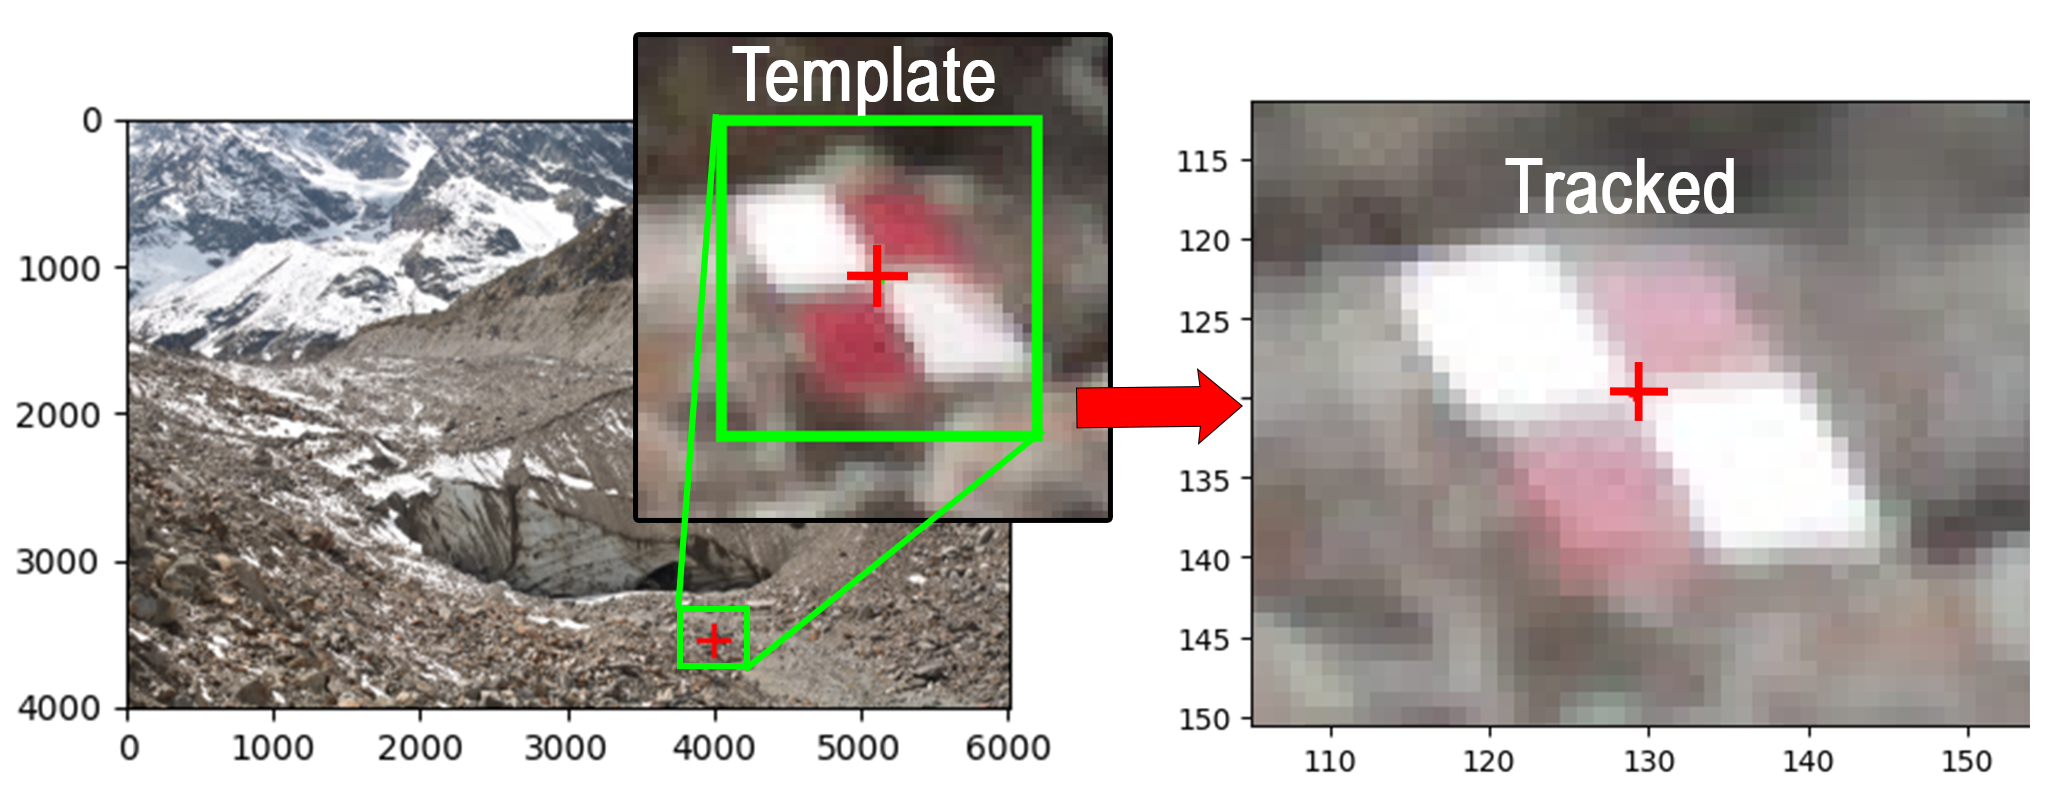
\includegraphics[width=1\textwidth]{tracking_gcp.png}
    \caption{Example of template matching used to track GCPs on a
        monocular image sequence. The green square represents the
        template on the reference image that is searched in all the other
        images of the sequence.
        The red cross marks the estimated position of the center of the
        template in a new
        image.}
    \label{fig:4:templatematch}
\end{figure}

\subsection{Stereoscopic image processing workflow}\label{sec:4:stereoworkflow}

\begin{figure}
  \centering
  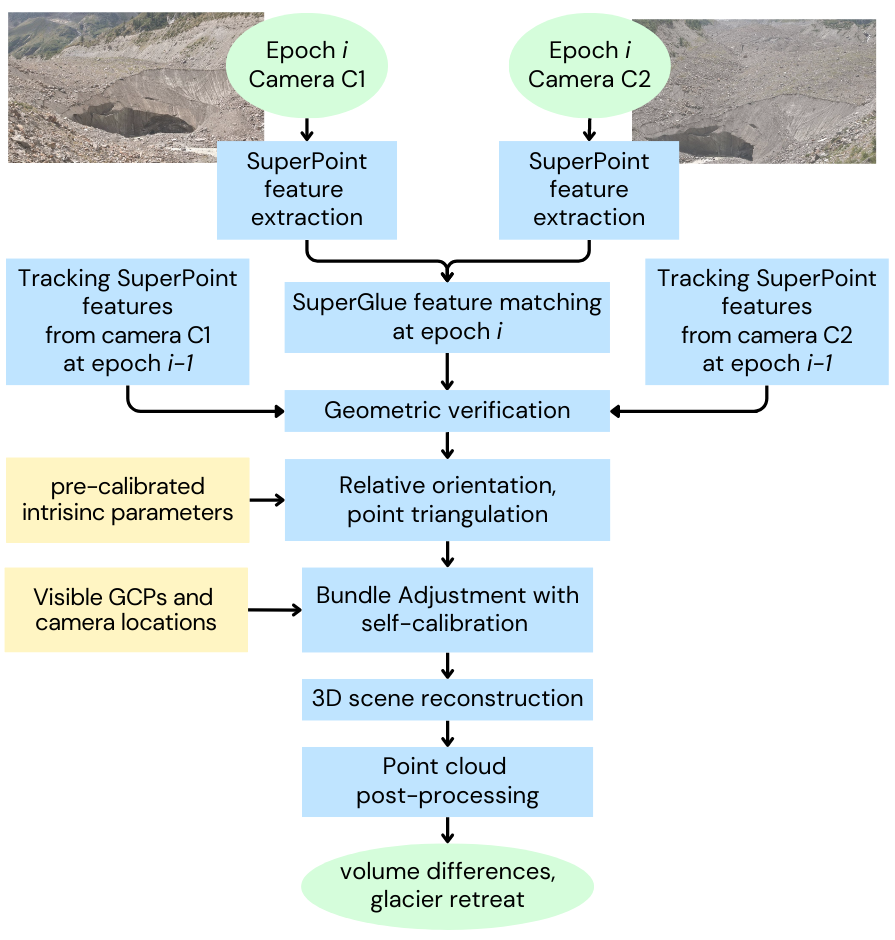
\includegraphics[width=.8\textwidth]{3_stereo-workflow.png}
  \caption{Scheme of the stereoscopic workflow performed with ICEpy4D. At a generic epoch \(i\), new features are extracted and matched. At the same time, features from the previous epoch \(i-1\) are tracked on the current epoch images. After geometric verification, features successfully matched are used for 3D scene reconstruction. Point clouds obtained on different days are used to compute ice volume differences and glacier retreat.}
  \label{fig:4:stereo-workflow}
\end{figure}

ICEpy4D was developed to achieve a daily stereoscopic reconstruction of the glacier snout.
ICEpy4D\footnote{\url{https://github.com/franioli/icepy4d})} is a Python-based toolkit that allows for solving different steps of scene reconstruction
(\figref{fig:4:stereo-workflow}). 
In particular, the main steps consist of:
(i) finding corresponding points by deep-learning feature matching;
(ii) tracking features on the sequence of images acquired from the same camera;
(iii) performing 3D scene reconstruction and point cloud post-processing.
All the processing was carried out with a mid-class workstation equipped with a 20-cores
i7-12700 CPU, 32~Gb of DDR5 RAM and a GPU NVIDIA RTX A2000 12~GB.

\subsubsection{Wide-baseline image matching}\label{sec:4:matching}

To find corresponding points, the combination of DL feature-matching algorithms
SuperPoint \citep{DeTone_2018} and SuperGlue \citep{sarlin2020superglue} was used and
fully integrated into ICEpy4D package.
SuperPoint is a Convolutional Neural Network (CNN) with an encoder-decoder
structure, which detects interesting points and computes 256-value descriptors in a
single forward pass.
\citet{DeTone_2018} trained SuperPoint to detect corner-like features first using corners
of synthetic shape datasets as ground truth.
They employed a self-supervised approach by applying random homographies to warped
copies of the input training images and combining the results \citep{DeTone_2018}.
SuperGlue is an attention-based graph CNN used for local feature matching.
It was specifically designed to match SuperPoint features based on their descriptors.
\citet{sarlin2020superglue} trained SuperGlue in a supervised manner and published two
different sets of weights: one for indoor environments and another for outdoor
environments.
The outdoor environment model was trained on the Megadepth dataset
\citep{Li_Snavely_2018_MegaDepth}.

The SuperPoint and SuperGlue models were not fine-tuned to ensure the replicability of
the proposed pipeline in different scenarios, without the need for a
dedicated ground truth dataset.
Acquiring a ground truth dataset may be can be challenging, especially for natural
scenarios and mountain environments.
Typically, generating datasets for training wide baseline matching requires collecting a
substantial number of image sequences with a normal baseline and artificially creating a
wide baseline by skipping intermediate images.
However, this approach would demand numerous field campaigns to capture series of UAV
images under different environmental conditions and throughout various seasons, making it
generally unfeasible.
Moreover, the matching results obtained with the Belvedere stereo pairs were already
satisfactory using pre-trained weights for outdoor environments without any fine-tuning
(see results in \secref{sec:4:res_matching}).

Since feature matching was performed on a GPU, which has limited memory, it was necessary
to decompose the full-resolution images into smaller tiles and match pairs of tiles one
after the other.
Therefore, a two-steps approach was implemented: first, a matching is performed with
SuperPoint and SuperGlue on downsampled images. Subsequently, the
full-resolution images were subdivided into regular tiles, and only the tiles that had
corresponding features in the low-resolution images were selected as candidates for a
second matching step.
In the second step, the selected tiles were matched using the same procedure as before.
The features matched in each tile were then reassembled to recover their image
coordinates on the original image for geometric verification.
Incorrectly matched keypoints, which did not satisfy the epipolar constraint, were
rejected using Pydegensac~\citep{Mishkin2015_pydegensac}, by imposing a maximum
re-projection error of 1.5 px.

\begin{figure}[ht]
  \centering
  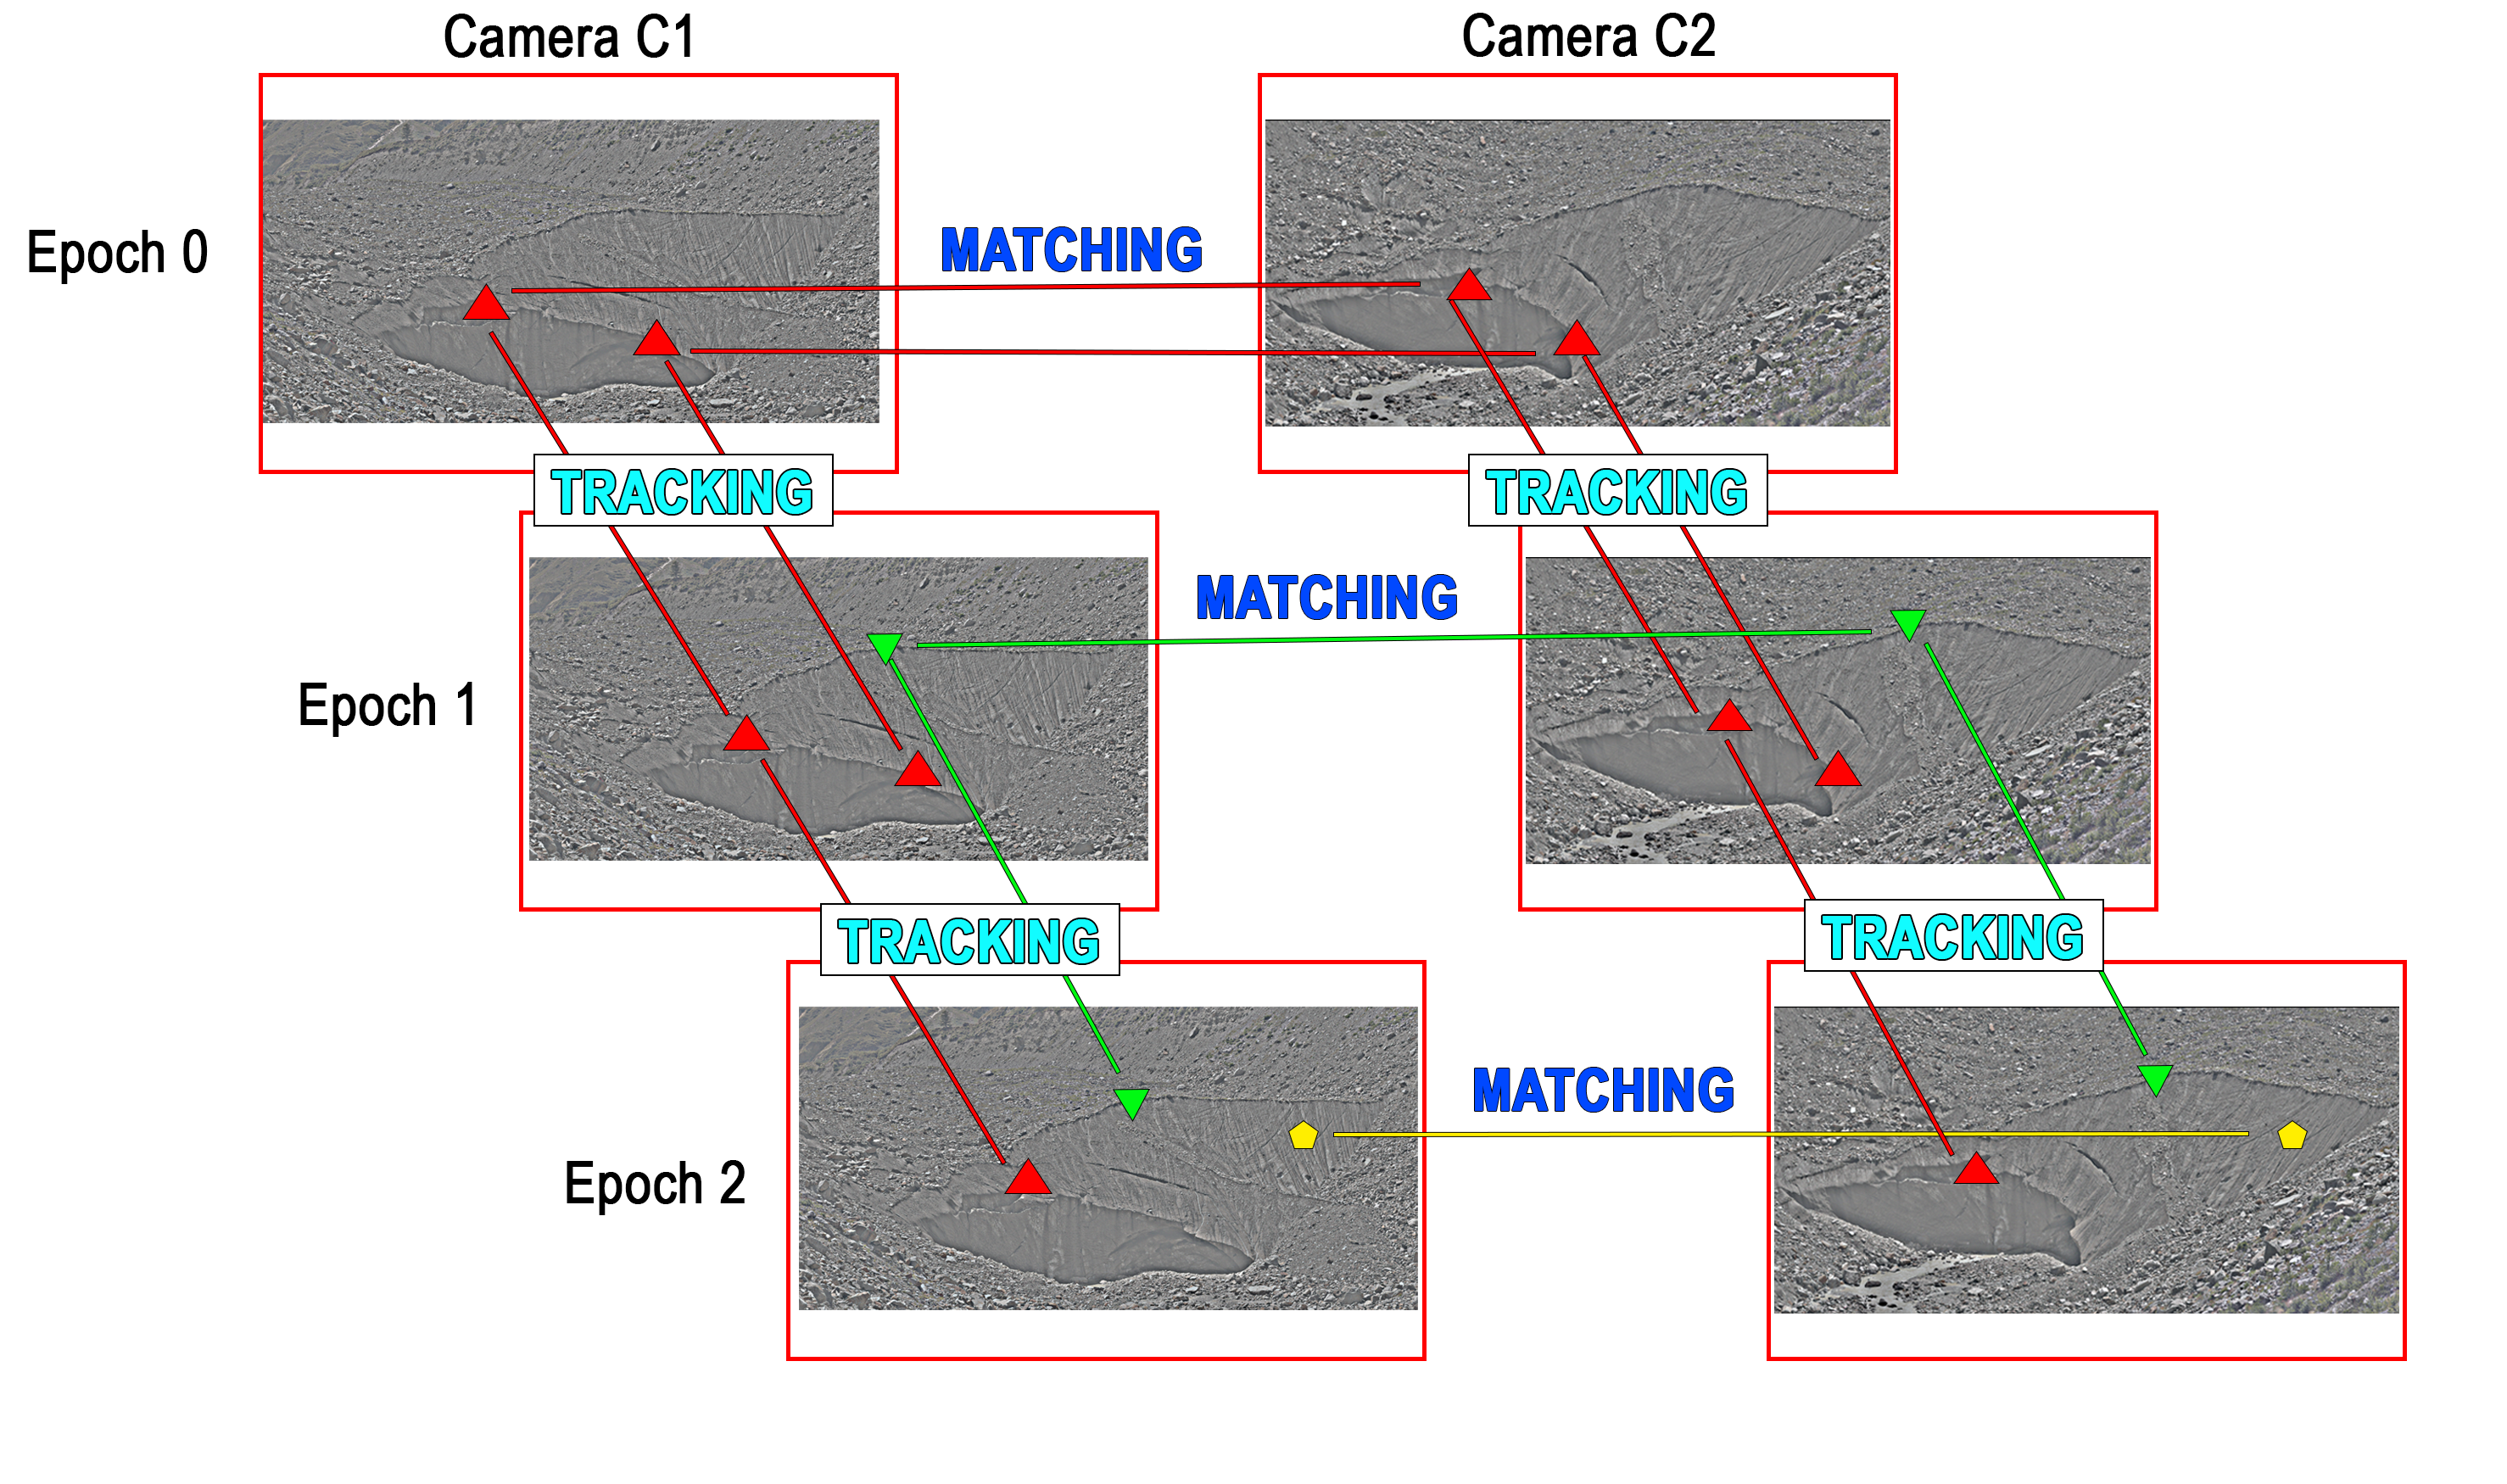
\includegraphics[width=0.8\textwidth]{3_tracking.png}
  \caption{Scheme of feature tracking in stereo-cameras sequence. At each epoch, new
    features are matched on the stereo pair (horizontal lines), but also tracked from
    previous epochs (oblique lines).
    At epoch 0, the matches are only the corresponding features matched
    between	current the stereo pair (red triangles).
    At epoch 1, the valid matches are the new corresponding features matched (green
    triangles) plus the successfully tracked features from epoch 0 (red triangles).
    The same holds for epoch 2, where the matches are the new
    corresponding features (yellow pentagons), plus the features tracked from both epoch
    0 and 1.}
  \label{fig:4:tracking}
\end{figure}

\subsubsection{Tracking points over epochs}\label{sec:4:tracking}

Matched points are tracked over time on single camera image time series
(\figref{fig:4:tracking}).
This procedure led to two main advantages: (i) increasing the number of matches
at every epoch; (ii) obtaining a time-series of corresponding points that can be
triangulated to derive their 3D coordinates over time.
For brevity, images are labeled with the camera labels \(C1\) and \(C2\), while a
superscript indicates the acquisition epoch.
At a generic epoch \(i\), keypoints were detected and
matched between images \(C1^i\) and \(C2^i\) with the procedure described
in \secref{sec:4:matching}.
SuperPoint features were then extracted on \(C1^{(i+1)}\) and \(C2^{(i+1)}\).
Valid matched features from \(C1^i\) were tracked to \(C1^{(i+1)}\), by matching their
descriptors with the SuperGlue algorithm.
The same holds for camera \(C2\).
If a matched feature at epoch \(i\) was tracked successfully both from images
\(C1^i\) to \(C1^{(i+1)}\) and from images \(C2^i\) to \(C2^{(i+1)}\), then this feature
was considered a valid match also for epoch \(i+1\) and merged to the new corresponding
features detected at epoch \(i+1\).
Duplicate features (e.g., a feature that was successfully tracked from epoch \(i\) to
epoch \(i+1\) but also matched again at epoch \(i+1\)) were removed and a new geometric
verification was carried out to reject outliers.

\subsubsection{3D scene reconstruction}\label{sec:4:3dreconstruction}

At each epoch, the reconstruction of the terminal ice cliff was carried out using ICEpy4D
in two main steps: (i) relative-absolute orientation, and (ii) bundle adjustment.
In the first step, matches between each stereo pair were utilized to estimate the
relative pose of the two cameras, based on the camera's pre-calibrated intrinsic matrix.
Subsequently, the absolute orientation was determined by calculating a Helmert
transformation, considering the cameras' locations and the available GCPs.
In the second step, a full BA was performed to refine the relative-absolute solution. For this purpose, the Agisoft Metashape software package was employed via its Python API.
The choice of Agisoft Metashape was driven by its support for GCPs, the possibility to
assign different a-priori weights to observations, and the availability of a Python API,
enabling the software to be run from a Python routine in headless mode.
The Metashape BA was seamlessly integrated into ICEpy4D, enabling the entire workflow
chain to run automatically without any interaction with the GUI.

During the BA, the cameras' locations and the available GCPs were used as observations.
A centimetric a-priori accuracy was assigned to the world coordinates of the GCPs.
A centimetric accuracy was also given to the camera locations to constrain their
positions, while still allowing for an estimation of the cameras' rotations.
Additionally, during the BA process, the principal distance of the
two cameras were refined by self-calibration based on the available GCPs, while the
remaining interior orientation parameters were kept fixed at their pre-calibrated values.

The dense reconstruction of the ice cliff terminus was again carried out using the
Agisoft Metashape API.
In fact, although Agisoft Metashape couldn't perform feature matching with wide baselines
due to its reliance on hand-crafted features, it was effective in performing dense
matching through semi-global matching
algorithms~\citep{Hirschmuller2012}, when accurate camera poses were available for image
rectification.
Depth maps were generated from full-resolution images (i.e., the highest
quality parameter in Agisoft Metashape) with mild filtering.
The estimated depth maps were then used to reconstruct a dense point cloud and a
triangulated mesh.


\subsection{Volume variation estimation}\label{sec:4:volumevariation}

\begin{figure}[ht]
\centering
  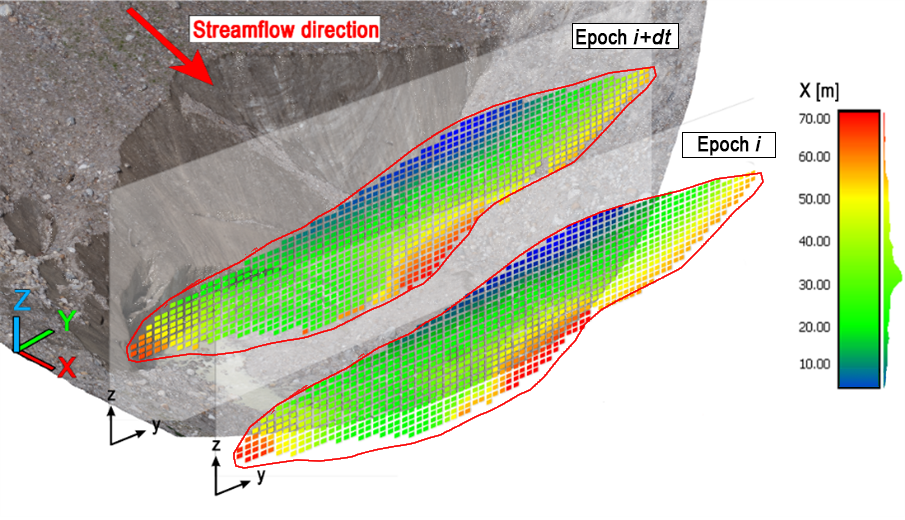
\includegraphics[width=1.0\linewidth]{3_dod_scheme.png}
  \caption{Scheme of Dem of Difference (DOD) approach used to compute volume variations
    at the glacier terminal ice cliff.
    Two point clouds built at epoch \textit{i} and \textit{i+dt} (we used dt=5 days to increase the signal-to-noise ratio), were rasterized to a vertical Y-Z planes, with normals parallel to the glacier flow direction (X direction).
    Before rasterization, the point clouds are clipped with the same convex polygon in
    the Y-Z plane (red line).
    The colors of the grids represent the depth of each cell of the two rasters along the X direction (i.e., the distance along X from a reference plane).
    Volume variation was computed by DOD of the two rasters along X.}
  \label{fig:4:dod_scheme}
\end{figure}

The daily variation of ice volume was determined by calculating the DEM of Differences
(DOD) along the streamwise direction. A local reference system was established by
defining the X-direction as the streamwise direction, the Z-direction as the geodetic
height, and the Y-direction to complete the right-hand reference system.
The point clouds of two different epoches were rasterized to a reference YZ plane,
corresponding to the frontal view of the terminal ice cliff, using a grid step of 0.3
meters, while maintaining the same raster origin and extent (i.e., the two point clouds
were first clipped with the same convex polygon).
The volume change between two epochs was then calculated by differentiating the
two rasters cell-by-cell (\figref{fig:4:dod_scheme}).
To account for possible incomplete coverage and holes in the 3D reconstruction, which may
result in volume underestimating, the computed volume difference was normalized by the
percentage of filled cells (i.e., cells with at least one point in the original point
cloud) in both rasters.
The normalization was computed as in Eq.~\ref{eq:4:volumevariation}:

\begin{equation}
  dV_{\text{norm}} = dV \times
  \frac{n_{\text{filled}}}{n_{\text{total}}}
  \label{eq:4:volumevariation}
\end{equation}

where \( n_{\text{filled}} \) is the number of filled cells in both the rasters and \(
n_{\text{total}} \) is the total number of cells within the clipping polygon.
During the considered study period, the percentage of filled cells in the rasterized
point clouds of the terminal ice cliff ranged from 90\% to
98.8\%, with a mean value of 96.8\%.


\subsubsection{Temporal lag between point clouds for volume and velocity estimation}
\label{sec:4:timelag}

To estimate volume variation and surface velocity, the point clouds were processed using
pairs spaced 5 days apart.
This interval was selected based on the available open data acquired by Ioli et al. with
historical aerial datasets and in-situ annual photogrammetric UAV surveys on the
Belvedere Glacier between 1977 and 2022~\citep{Ioli2022,ioli_2023_zenodo,Degaetani2021}.
Given a decimetric accuracy of the stereo point clouds (see the results presented
in \secref{sec:4:res_uav_validation}), a 5-day interval was considered appropriate to
achieve a good signal-to-noise ratio.
Therefore, each point cloud acquired on a particular day was compared to that captured
5 days earlier for volume differences computation.
However, in case of adverse weather conditions which hindered stereo reconstruction and
resulted in the unavailability of a point cloud on a certain date, the closest one
acquired within a range of 5 to 7 days earlier was chosen as a substitute.
This approach ensured a balance between preserving temporal resolution and minimizing
data gaps caused by unfavorable weather conditions.

To ensure consistency between volume variations and surface velocities, the same pairs of
days utilized for estimating volume differences from point clouds were also employed for
selecting pairs of images to compute surface velocities using DIC on a monoscopic image
sequences (see \secref{sec:4:dic}).

\subsection{Automatic extraction of ice cliff top edge}
\label{sec:4:topedge}
To calculate the glacier retreat over time, the top edge of the ice cliff was chosen as a
reference point.
This decision was made because the top edge remained rather stable and experienced
limited changes in morphology compared to the rest of the terminal ice cliff, which is
often affected by deformation and other processes that altered its shape, such as ice
block collapses.

The top edge of the ice cliff was automatically extracted from point clouds, by
exploiting geometric features of each point with respect to its neighborhood
~\citep{Hackel2016}.
To identify elongated features situated at the edges of the ice cliff within the point
cloud, the linearity and normal change rate were computed for each point with respect to
a neighborhood sphere of radius 2 m. By employing empirically determined thresholds
specifically tailored to the study site, these geometric properties facilitated the
identification and extraction of the top edge of the glacier terminus from the point
cloud data.

\subsection{Digital Image Correlation from single cameras}
\label{sec:4:dic}
DIC allows for determining the displacement of an image patch between two images (master
and slave) of the same scene and acquired at different epochs by the same camera. The
displacement \(d\) is obtained as  (Eq.~\ref{eq:4:dic}):

\begin{equation}
  d = \text{argmax}_{(r,q)} S(A(i,j),B(i+r,j+q))
  \label{eq:4:dic}
\end{equation}

where \(S\) is a similarity function, \((i,j)\) are the coordinates of the master patch
\(A\), and \((r,q)\) are the coordinates of a search area around the slave patch \(B\).
In our study, we adopted the open-source Local Adaptive Multiscale image Matching
Algorithm (LAMMA) written in Matlab \citep{Dematteis2022}.
LAMMA adopts a hierarchy structure of patch grids of increasing spatial resolution and
uses locally-adaptive search area sizes, according to the displacements already
obtained in the neighboring region.
LAMMA allows faster computation and reduces the occurrence of outliers compared to
traditional DIC processing \citep{Dematteis2022}. As a correlation function, we used the
cosine similarity applied to orientation images \citep{Dematteis2021}, which is less
sensitive to changes in the shadow pattern and it is known to perform well in glacier
environments \citep{Heid2012_evaluation_xcorr}.

We applied DIC to the undistorted images which were corrected according to the interior
orientation parameters estimated at every epoch within stereo BA.
Moreover, assuming a zero-translation of the camera perspective centers, but only small
rotations (\secref{sec:4:stability}), the transformation between the image plane at an
arbitrary epoch with respect to a reference one (named \textit{master}) is
described by a homography transformation.
As a master image, we adopted the image taken on 28/07/2022, which was
coeval with the DSM built from the UAV-A survey.
All the other images acquired were warped to be coregistered to the master image,
by computing a homography transformation \(H\) (Eq.~\ref{eq:4:homography}):

\begin{equation}
  H = KRK^{-1}
  \label{eq:4:homography}
\end{equation}

where \(K\) is the camera intrinsic matrix and \(R\) is the relative
rotation between the image planes \citep{forstner2016}.
The relative rotation \(R\) between the camera pose at a generic epoch and the pose of
the master camera was known from stereo processing.

The same image pairs used for volume  variation computation, spaced by a time lag of 5
days, were selected for DIC~(\secref{sec:4:timelag}).
The resulting displacement maps on the image plane, in pixel units, were finally
post-processed using a local filter to remove outliers.
To geocode the displacement maps, we used the open-source ImGRAFT Matlab toolbox
\citep{Messerli2015}.
Given a set of camera interior parameters (from stereo automatic calibration), ImGRAFT
allows the projection of 3D world coordinates \((x,y,z)\) into the 2D image coordinates
and the back projection of image coordinates onto a DSM, expressed as \(f(i,j) \to
(x,y,z)\). Thereby, the metric conversion of the image displacement vectors, with
components \((du,dv)\), is obtained by \(v(dx,dy,dz) = f(i+du,j+dv)-f(i,j)\), where
\(v\) is the 3D displacement vector. The \(f\) function is a form of ray tracing, carried
out based on the input DSM and the interior and exterior camera parameters
\citep{Messerli2015}.
To estimate the transformation between 2D and 3D coordinate systems,
we adopted the DSM acquired by UAV photogrammetry on 28/07/2022,
resampled at 1 m resolution to smooth small local DSM variations.
% The exterior orientation of the master camera was estimated based
% on a set of 6 markers with known image and world coordinates, distributed over the
% northern lobe. As the sequence of images was previously coregistered onto the master
% camera, the estimated exterior orientation was kept fixed for all the other epochs.

\begin{figure*}[ht!]
  \centering
  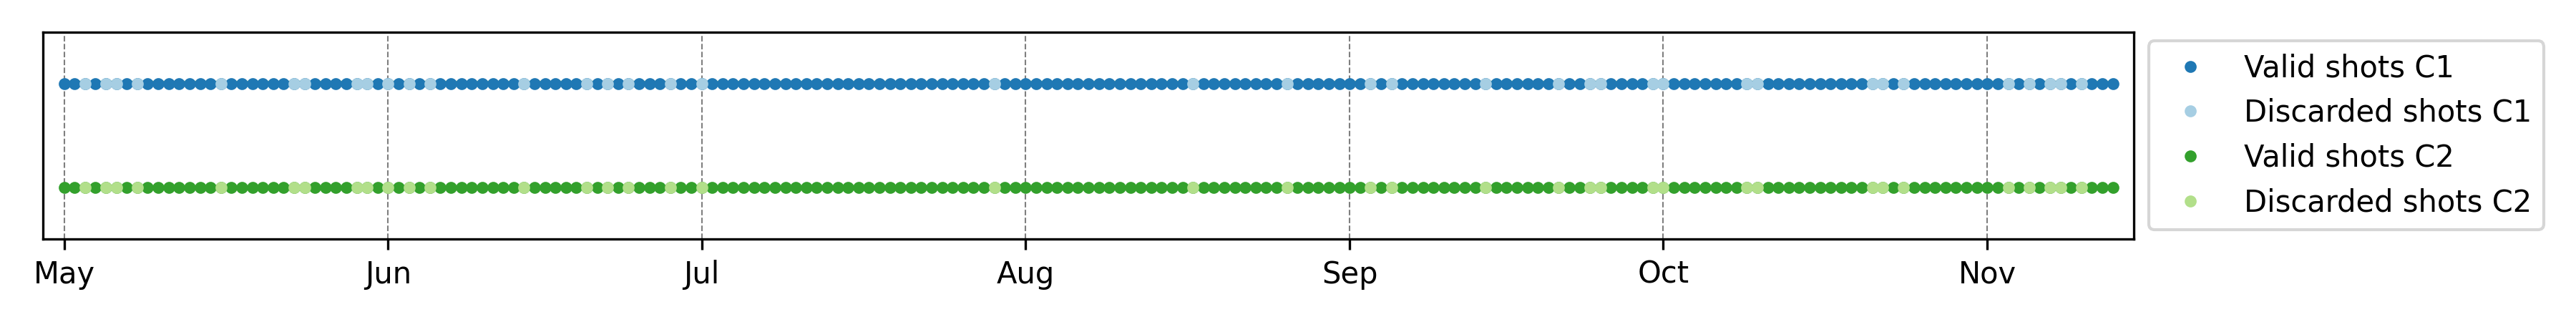
\includegraphics[width=162mm]{4_discardes_shots.png}
  \caption{Days with images acquired by the two cameras C1 and C2. Valid shots are
    represented with dark colors, while discarded days due to bad weather conditions are
    represented with light colors.}
  \label{fig:4:discardes_shots}
\end{figure*}

\subsubsection{Orthorectification uncertainty}
\label{sec:4:orthorectification_uncertainty}

The orthorectification of the 2D DIC displacement vectors to obtain 3D vectors is
influenced by the chosen DSM and its associated uncertainty \citep{Travelletti2012}.
Ideally, using an updated DSM derived from daily stereo-processing, as performed in
\citet{Marsy2020}, would be the optimal approach.
However, due to the camera's viewing location, it was not feasible to reconstruct the
daily DSM of the upper surface of the glacier lobe. Consequently, we utilized the UAV-A
DSM acquired on 28/07/2022.

To estimate the uncertainty derived by the use of a single DSM over the study period, we
conducted the following experiment: using the DSM of 28/07/2022 as the reference, we
virtually translated the glacier DSM along the flow direction to create two synthetic
DSMs representing the most advanced and the most retreated positions that the glacier
snout experienced in 2022.
The selection of these positions was based on the actual results of the stereo-processing
(\secref{sec:4:res_volumes_retreat}): the most advanced location of the snout was
approximately 12 meters
downstream (May 2022), while the most retreated location was about 5 meters upstream
(November 2022). This rigid translation of the glacier body not only affected the front
position but also resulted in a variation in the glacier surface elevation, i.e.,
thinning in the case of retreat.
Subsequently, we back projected the DIC displacement values of 28/07/2022 onto the
original DSM and the two synthetic DSMs. Finally, we compared the metric displacement
values considering the Median Absolute Deviation (MAD) between the original and synthetic
results.

\subsection{Correlation between glacier dynamics and meteorological variables}
\label{sec:4:meteoanalysis}
We compared the behavior of glacier velocity and ice volume loss at the snout with the
mean daily air temperature, precipitation and incoming solar radiation measured by the
AWS located ~2 km from the glacier terminus (\secref{sec:4:meteostation}).
Since both volume loss and velocity were obtained by comparing point clouds and images
acquired with a temporal lag of five days, we applied a moving average with a window of
five days to the weather data. Subsequently, to filter out the main signal due to the
seasonal trend, we detrended the time series by subtracting a robust loess smoothing
function~\citep{Cleveland1979} evaluated on a period of 180 days.
Finally, we calculated the Spearman correlation with the original data and obtained
residuals, which indicates how well the relationship between two variables can be
described using a monotonic function.
We adopted the Spearman correlation because it is more robust against outliers compared
to the linear correlation and because it allows the modelling of any kind of correlation
(i.e., linear and non-linear) between meteorological variables, ice volume losses and
glacier surface velocities.


\section{Results}\label{sec:4:results}

\subsection{Image acquisition}\label{sec:4:res_images}

During the snow-free study period (from 1/05/2022 to 13/11/2022), both camera C1 and
camera C2 were able to acquire images every day, for a total of 197 images. However, 39
images were discarded due to bad weather conditions, such as rain, low clouds, or fog,
resulting in 158 days with valid data for stereo and monoscopic processing
(\figref{fig:4:discardes_shots}).

\subsection{Automatic detection of GCPs}\label{sec:4:res_gcptracking}

Automatic target tracking of GCPs on monocular image sequences allowed successful
tracking of GCPs
in 99\% of image sequences from both the cameras.
Only in two out of 158 epochs did template matching fail, requiring target manual
collimation.
To validate template matching results, manual collimation was performed on all the
images.
For camera C1, the MAD between the image coordinates of the automatically tracked targets
and the manually collimated one was 0.46 px, with a standard deviation of 0.25 px.
Similarly for camera C2, the MAD was 0.55 px, with a standard deviation of 0.23 px,
denoting a sub-pixel accuracy of the template matching routine.

\subsection{Wide-baseline feature matching and tracking}\label{sec:4:res_matching}

\begin{figure}
  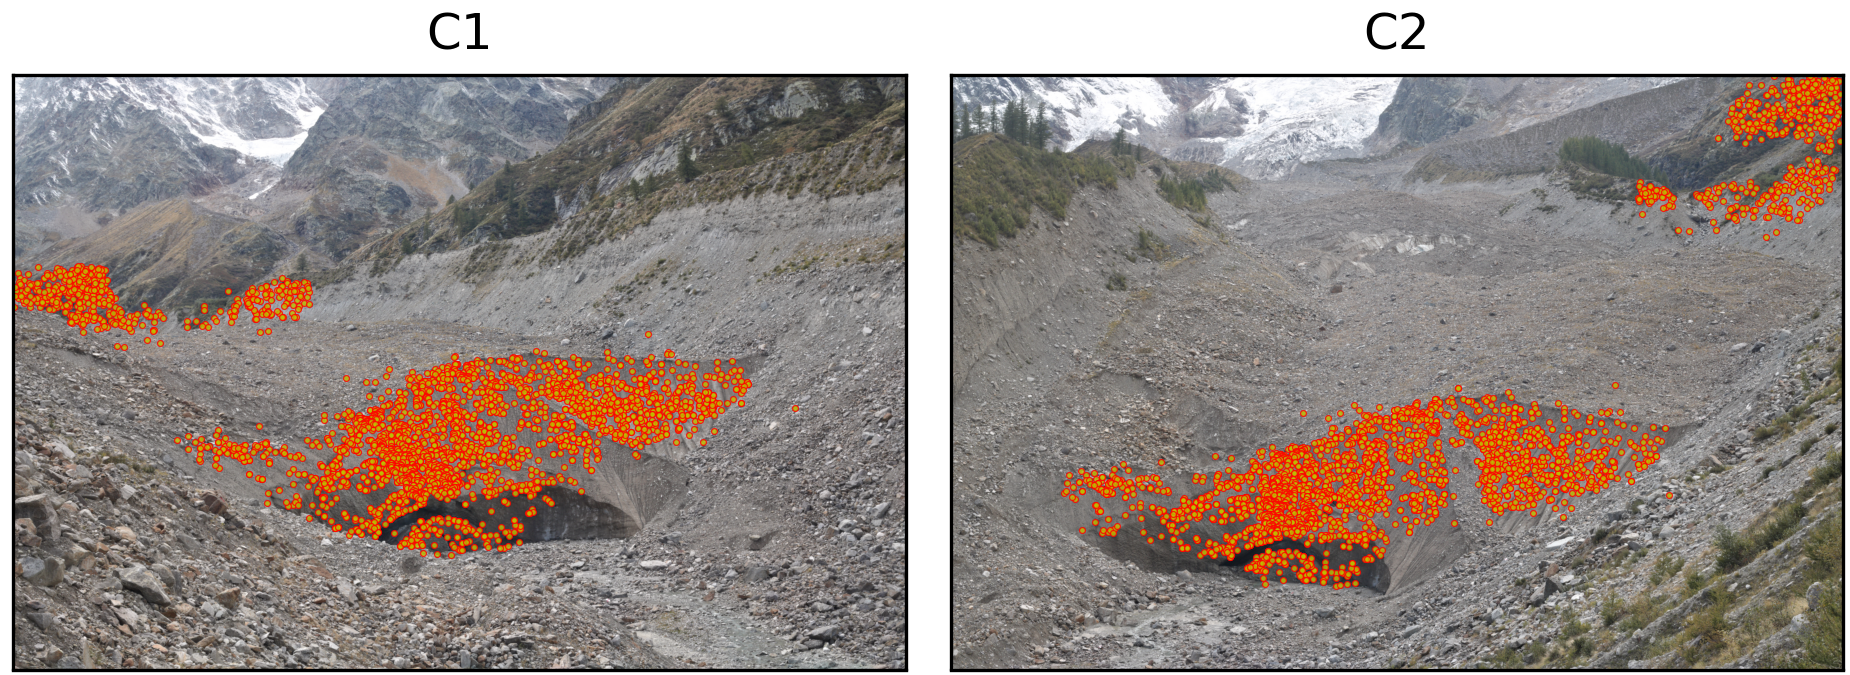
\includegraphics[width=1.0\linewidth]{4_matches_2022_09_27.png}
  \caption{Example of features successfully matched on the stereo-pair acquired on
    27/09/2022.}
  \label{fig:4:matches}
\end{figure}

\begin{figure}
  \centering
  \subcaptionbox{\label{fig:4:matches_stats:number}}{
    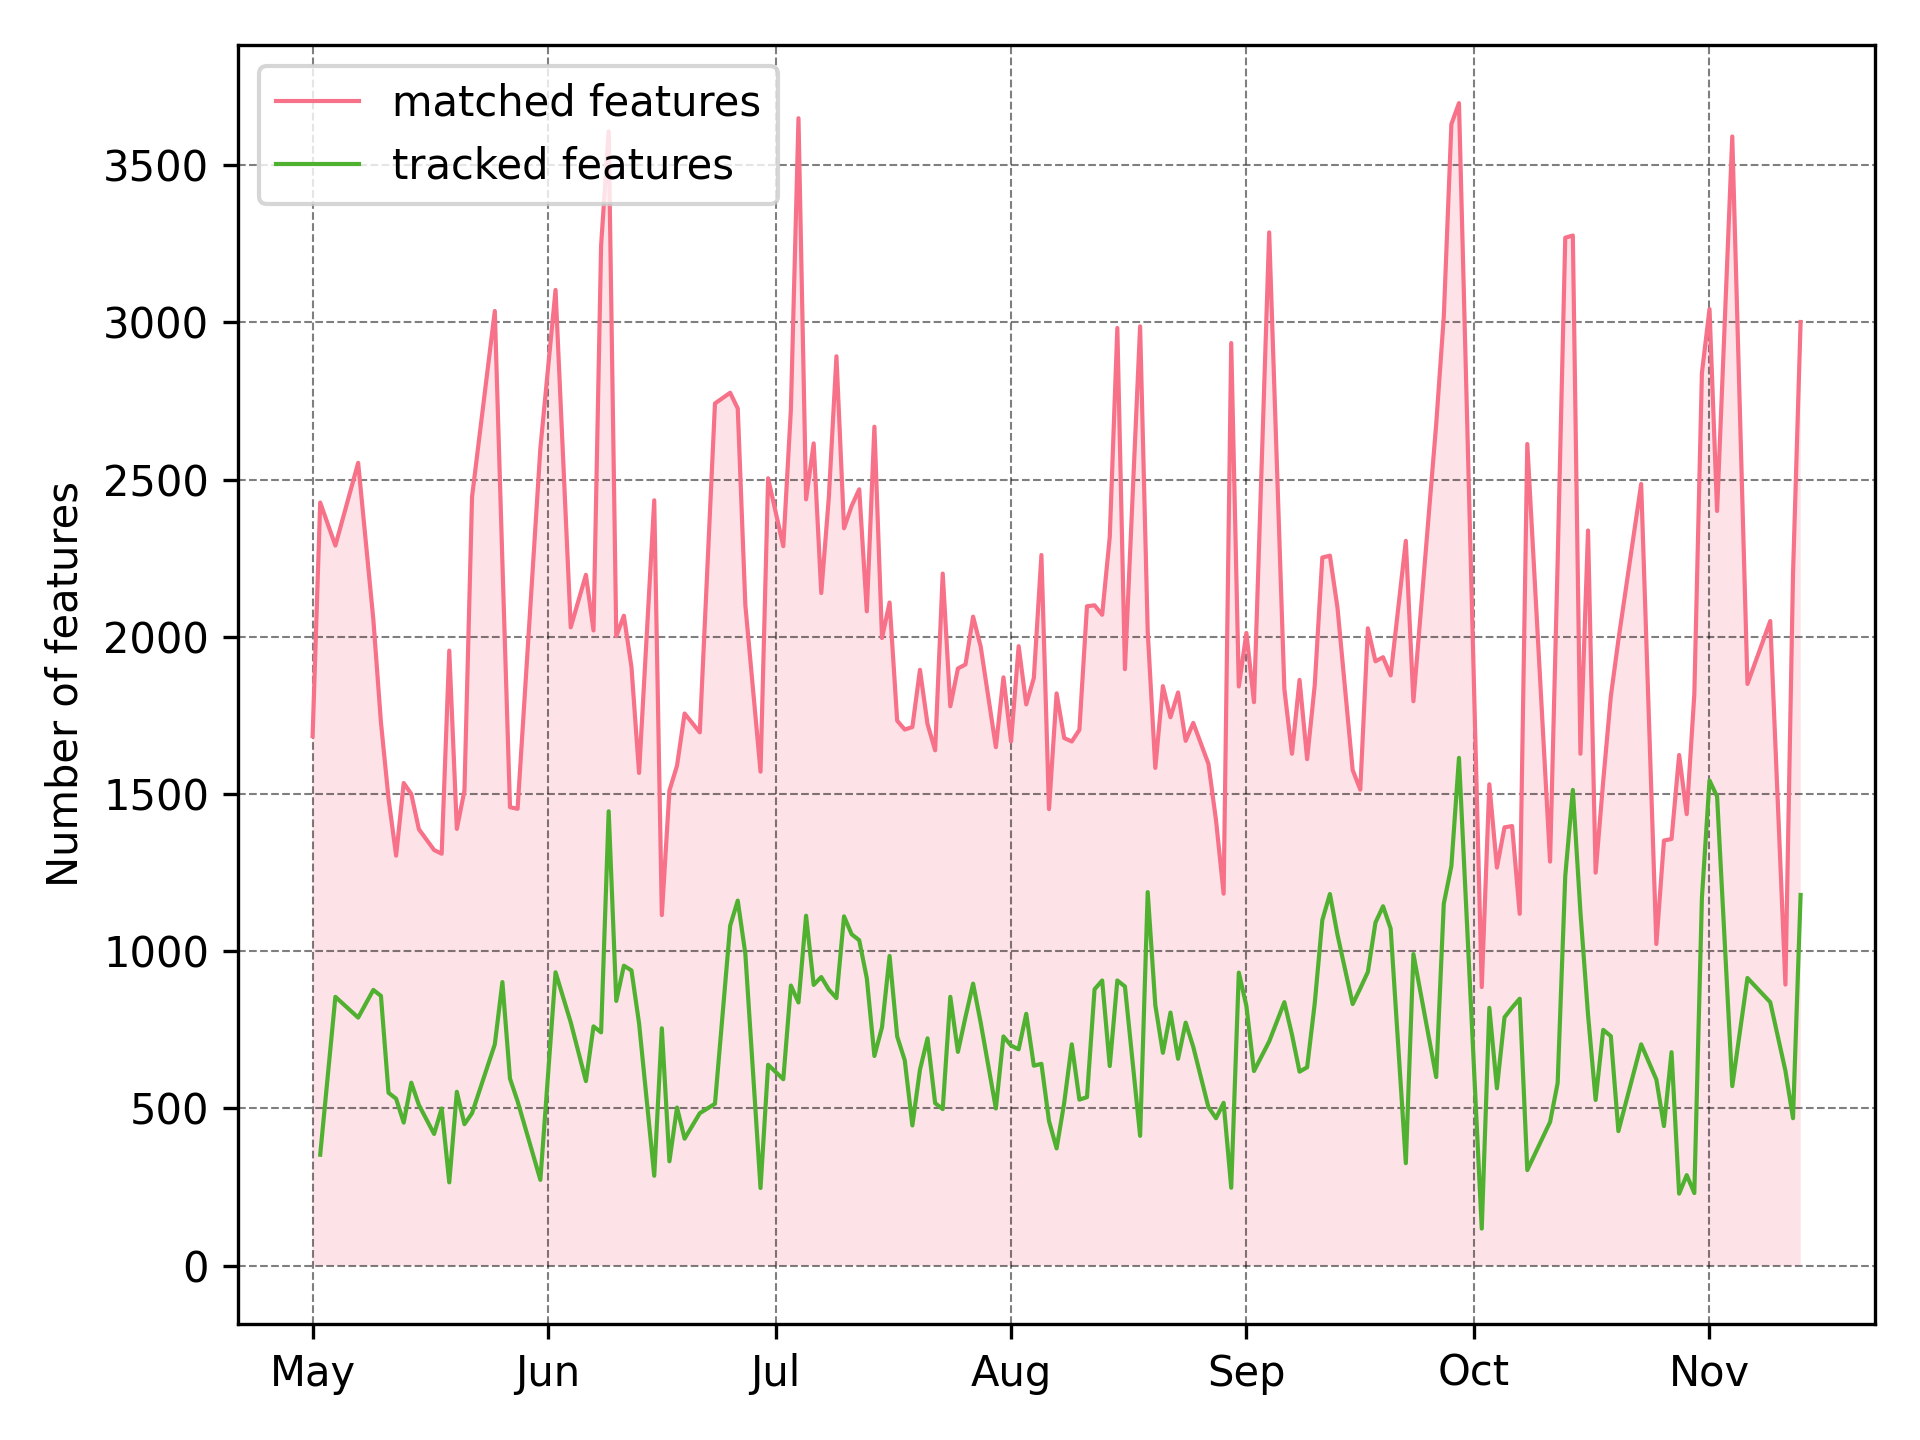
\includegraphics[width=.48\textwidth]{4_matching_tracking_stats.png}
  }
  \subcaptionbox{\label{fig:4:matches_stats:err}}{
    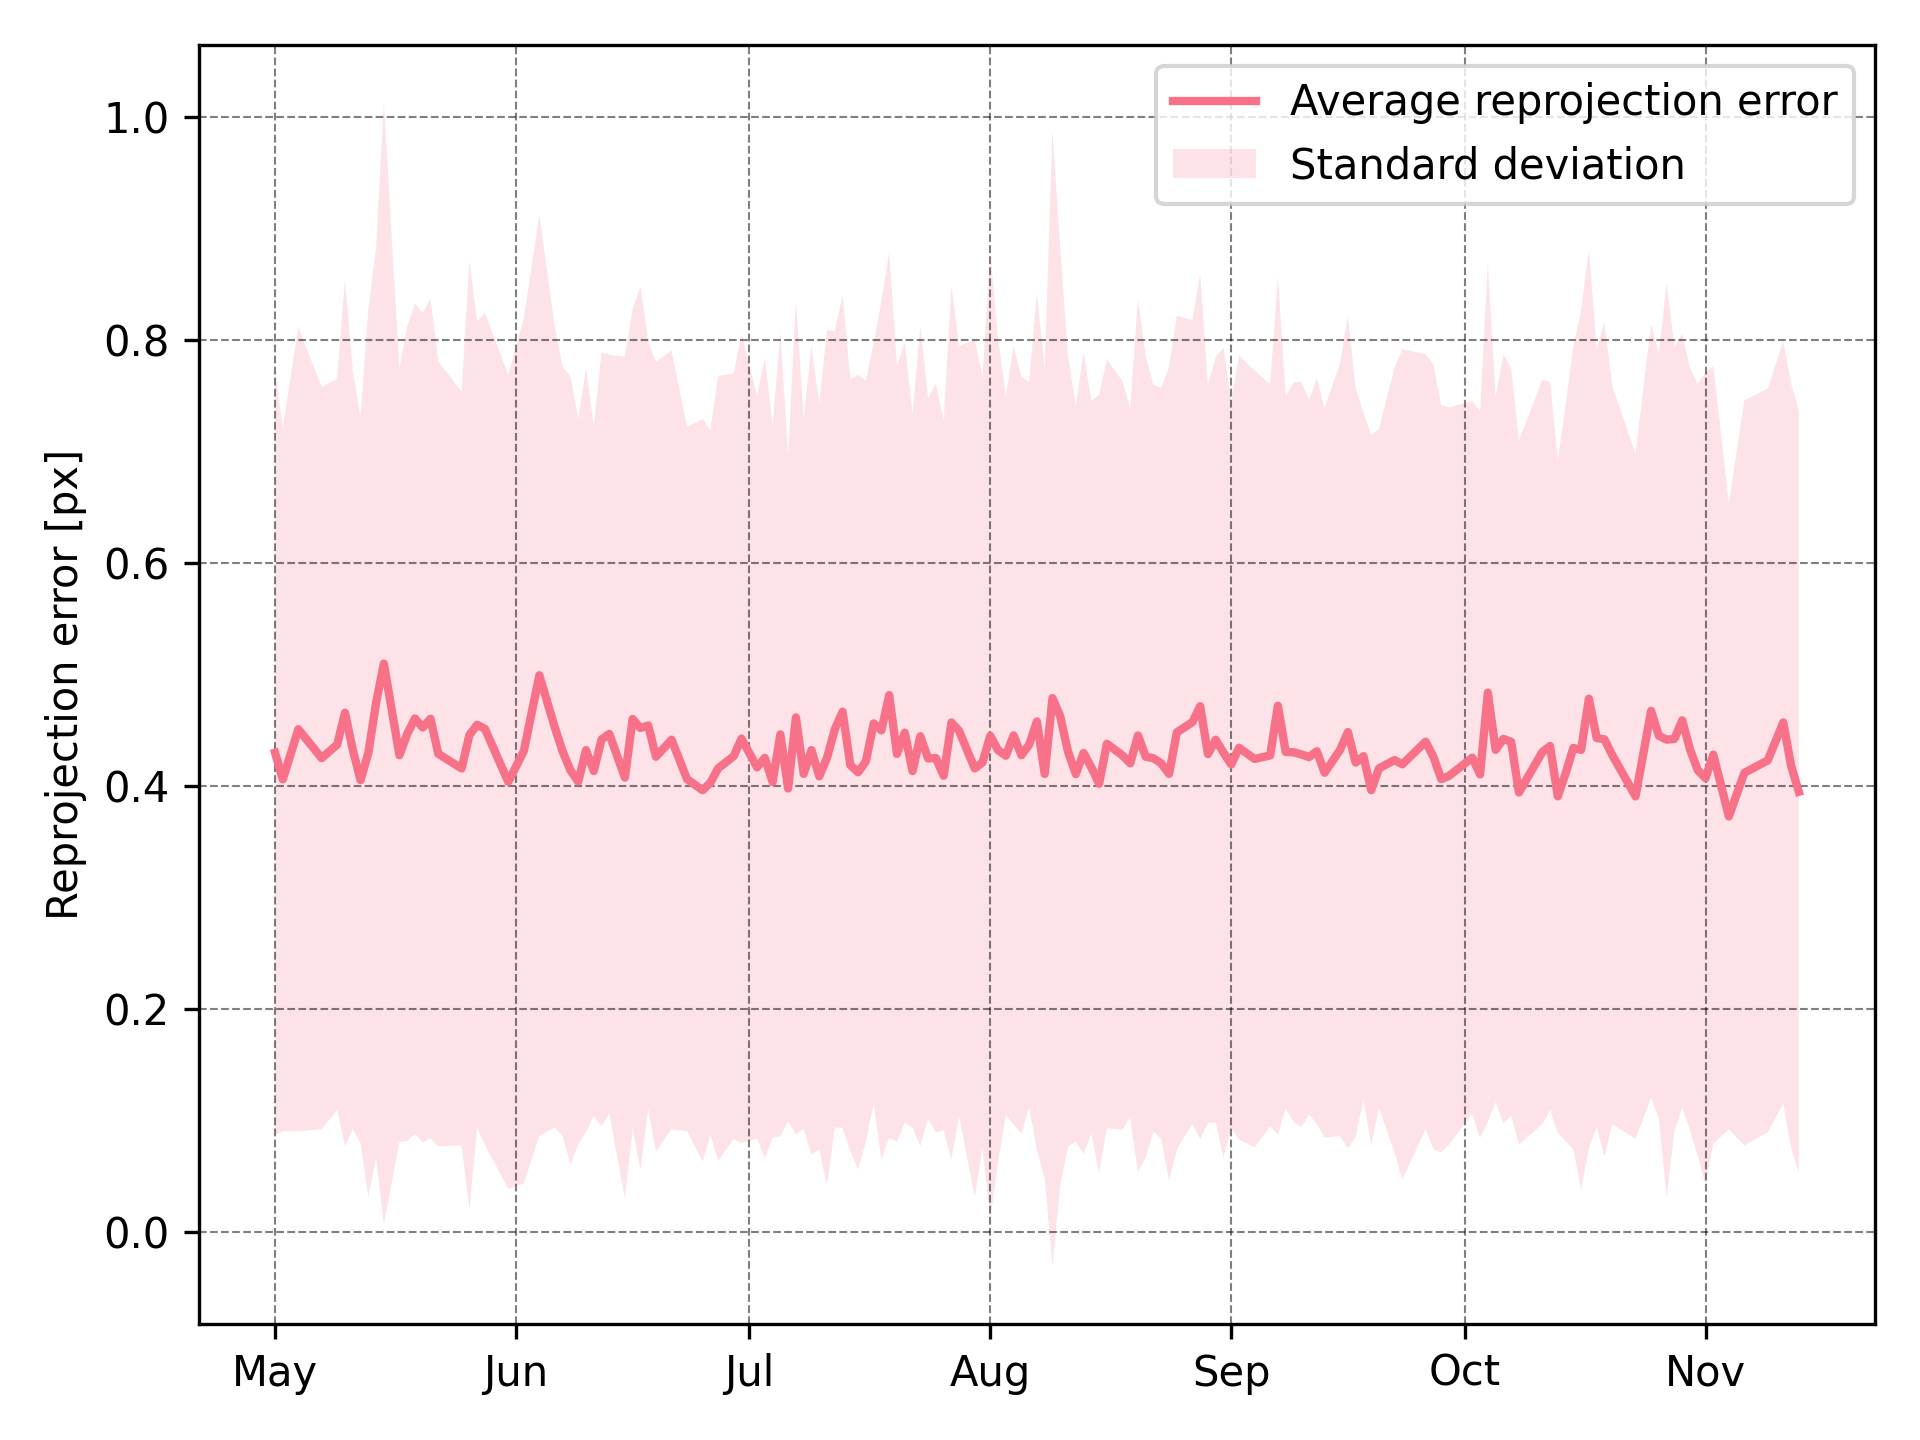
\includegraphics[width=.48\textwidth]{4_reprojection_error.png}
  }
  \caption{(a) Number of valid matches extracted from the stereo pair at each epoch and
    number of points tracked from the previous epoch.
    (b) Average and standard deviation of the reprojection error
    obtained by projecting the 3D coordinates of the tie points to the images.
    The average reprojection error was computed as the mean
    reprojection error for all the point on the two images.}
  \label{fig:4:matches_stats}
\end{figure}

The features matched by ICEpy4D on each stereo pair extended over the entire
frontal ice cliff, with some features detected in overlapping regions along the
streamwise left moraine (\figref{fig:4:matches}), near targets T1 and T2
(see \figref{fig:4:studyarea}b).
For each epoch, a number of features ranging from 1000 to 3500 were successfully matched
and validated following geometric verification (\figref{fig:4:matches_stats:number}).
Among them, approximately 30-40\% of the matched features were effectively tracked
from previous epochs, increasing the total number of matches available for
camera pose estimation while establishing a linkage between consecutive epochs.

After BA, the global average reprojection error was computed by projecting the 3D
coordinates of all the tie points to the two images and averaging
the norm of the reprojection errors for all the points.
\figref{fig:4:matches_stats:err} show the global reprojection error, which exhibited a
consistent fluctuation around 0.45 pixels, with a standard deviation of approximately 0.3
pixels.

\begin{figure}
  \centering
  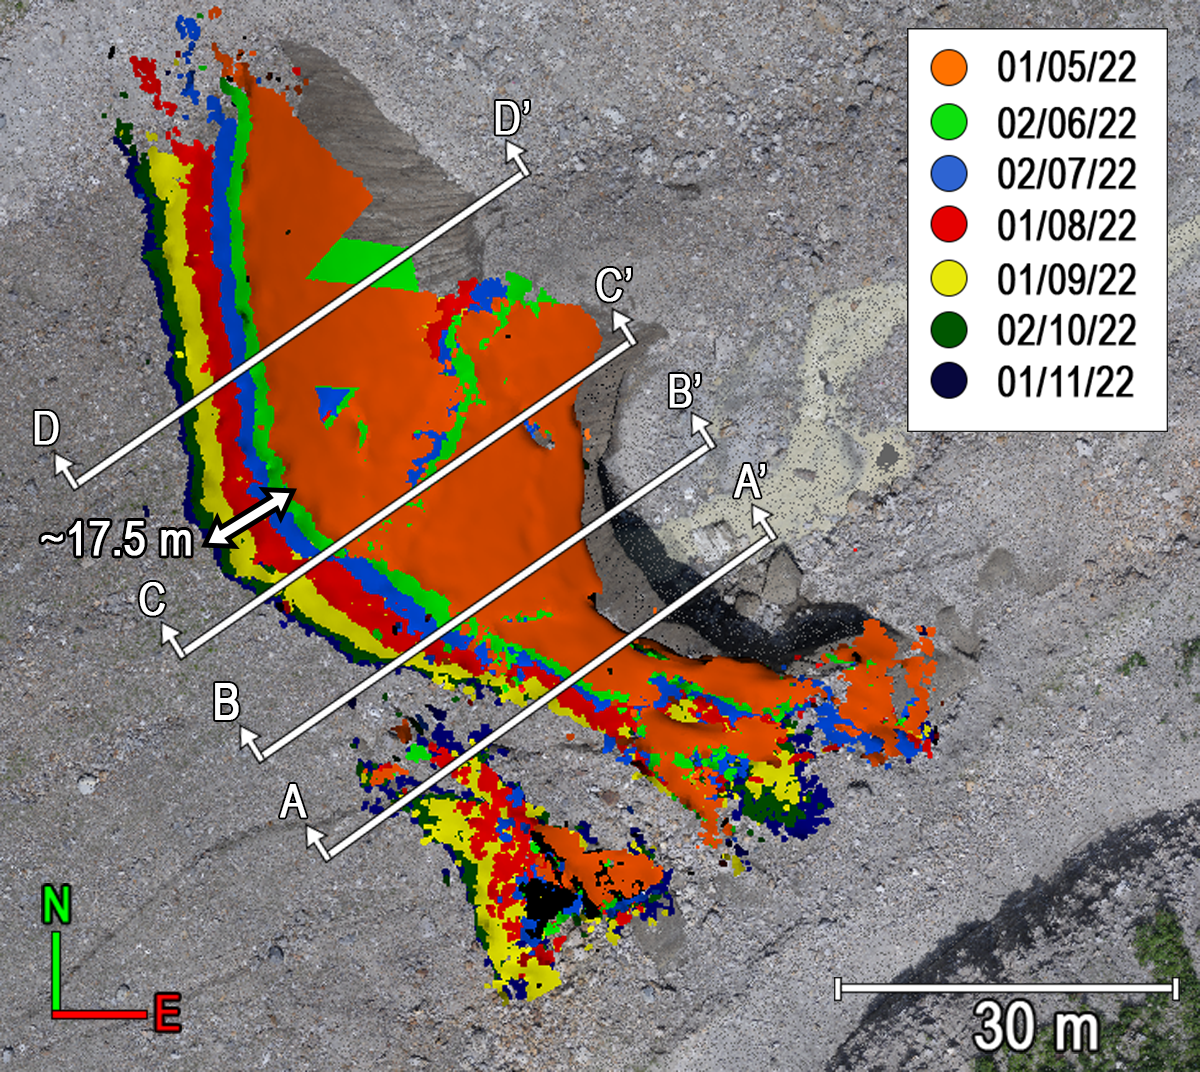
\includegraphics[width=72mm]{4_sec_location.png}
  \caption{Series of the point clouds built at the beginning of each month from
    01/05/22 to 01/11/22. The basemap is derived from a previous UAV survey carried out by the authors in July 2022}
  \label{fig:4:section_locations}
\end{figure}

\begin{figure}
  \begin{center}
    % \includegraphics[width=70mm]{sec4/sec_location} \\
    % \centering{(a)} \\ \vspace{1mm}
    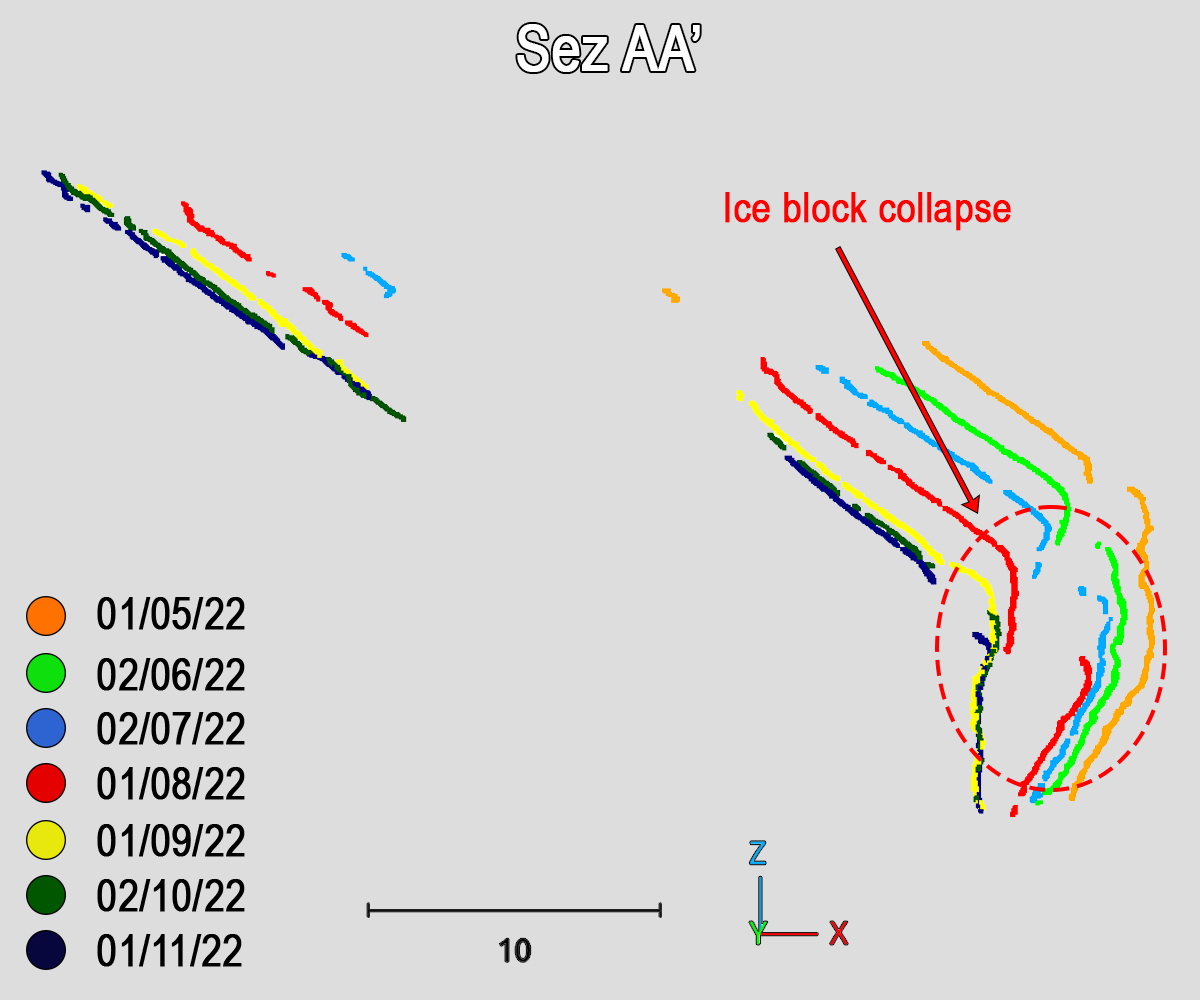
\includegraphics[width=70mm]{4_sec_aa.png} \quad
    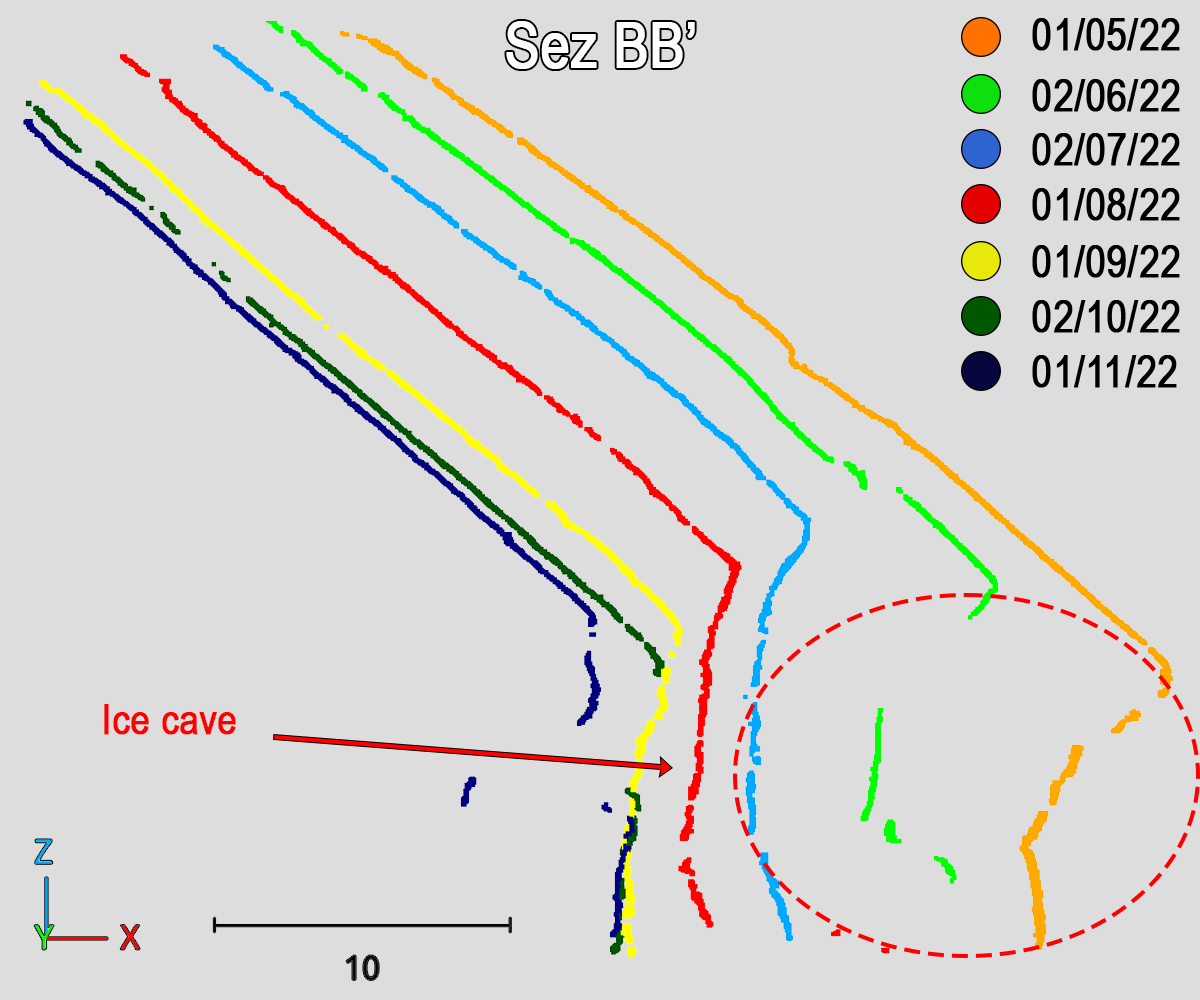
\includegraphics[width=70mm]{4_sec_bb.png} \\
    \centering{(a)} \hspace{70mm} \centering{(b)} \\ \vspace{1mm}
    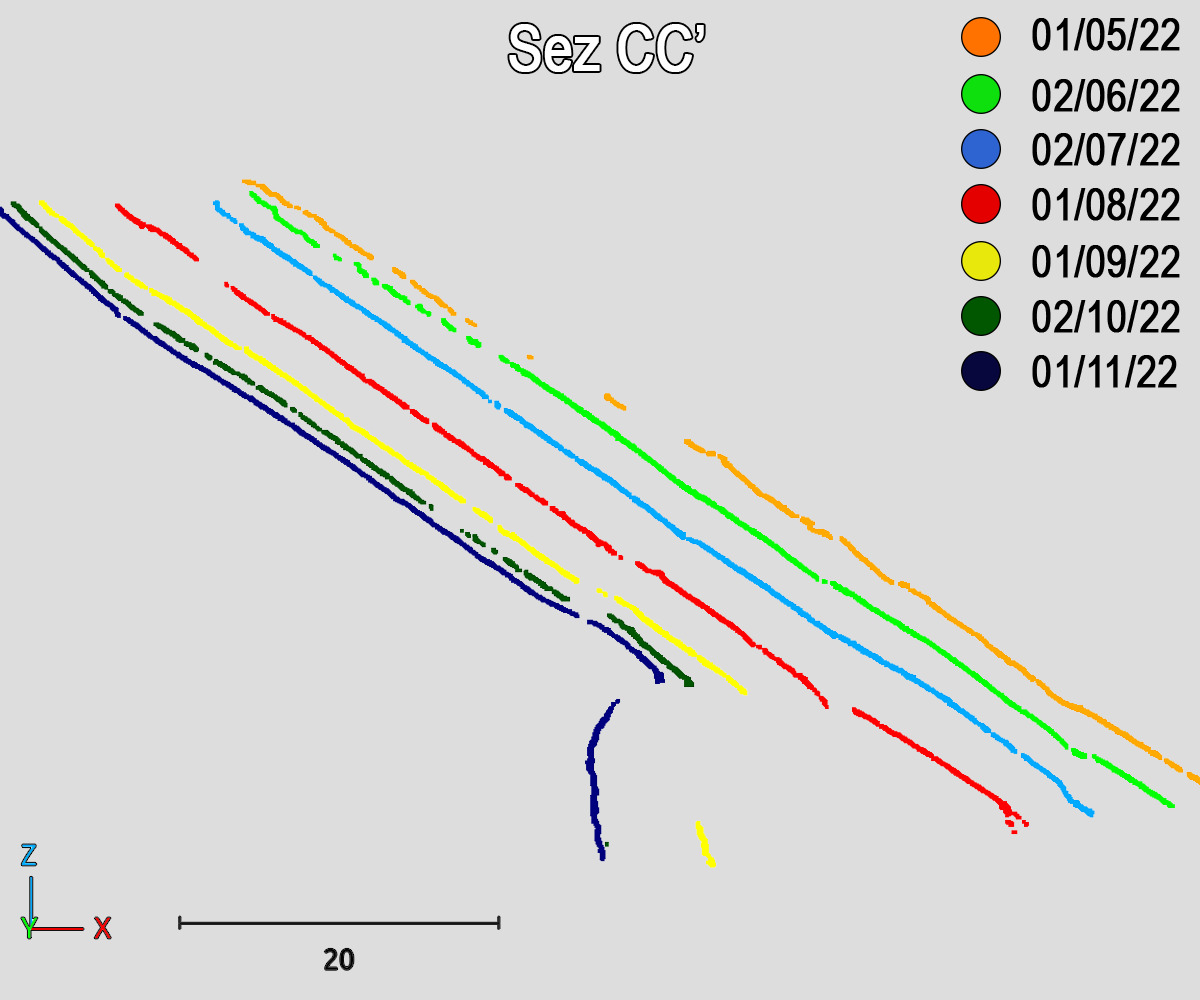
\includegraphics[width=70mm]{4_sec_cc.png} \quad
    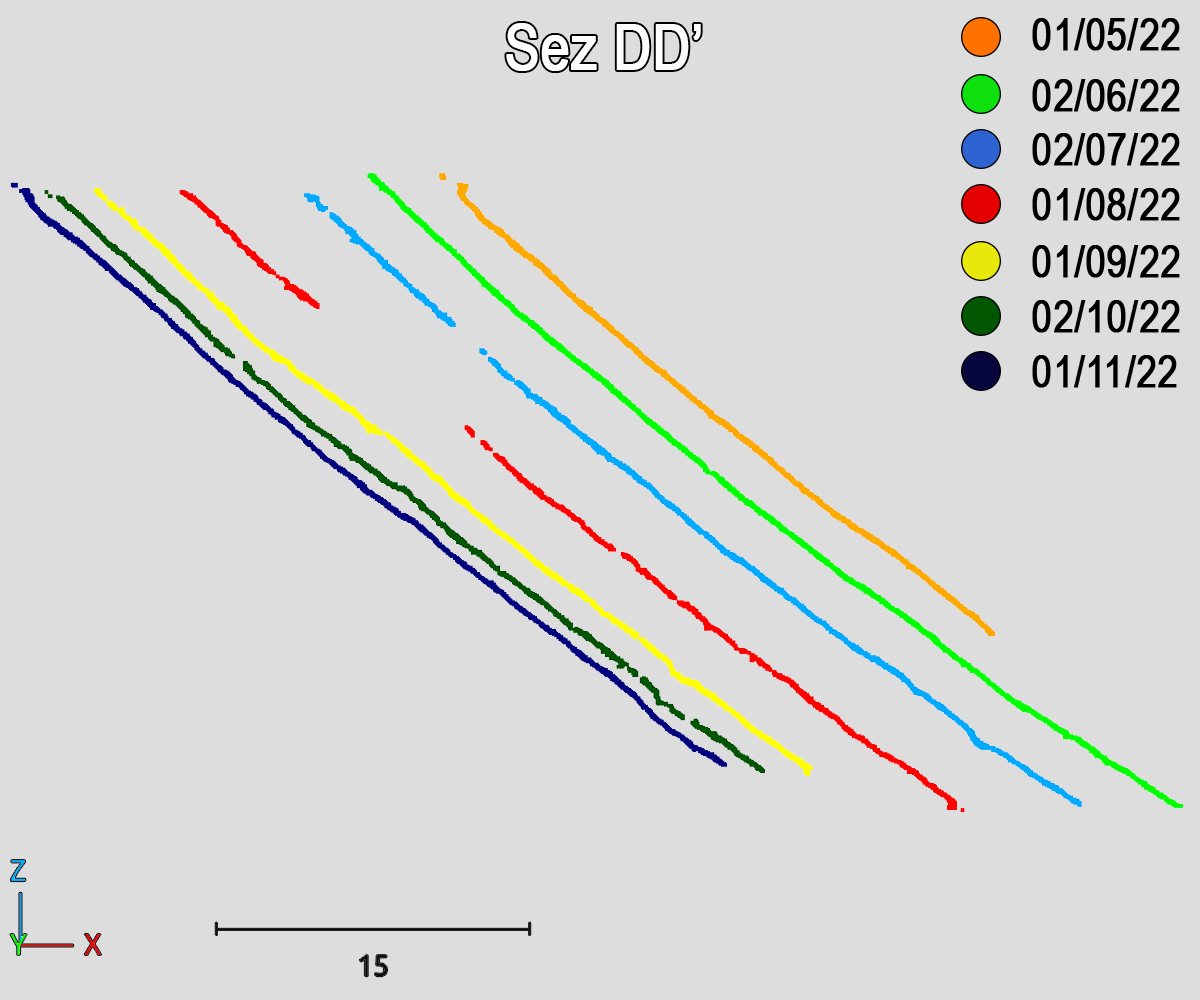
\includegraphics[width=70mm]{4_sec_dd.png} \\
    \centering{(c)} \hspace{70mm} \centering{(d)}
  \end{center}
  \caption{Vertical cross-sections extracted at the location marked in
    \figref{fig:4:section_locations}.
    All the cross-sections are extracted in a local reference system, with the
    X-direction pointing in the direction of the glacier flow, the Z-direction pointing upward, and the Y-direction completing the right-hand reference system.
    Please, note the different scales of the figures, indicated by the scale bar (in
    meters).}
  \label{fig:4:sections}
\end{figure}

\subsection{3D scene reconstruction}\label{sec:4:res_3dreconstruction_results}

% \begin{figure*}[ht!]
%   \begin{center}
%     \includegraphics[width=70mm]{sec4/sec_location} \\
%     \centering{(a)} \\ \vspace{1mm}
%     \includegraphics[width=70mm]{sec4/sec_aa} \quad
%     \includegraphics[width=70mm]{sec4/sec_bb} \\
%     \centering{(b)} \hspace{70mm}
%     \centering{(c)} \\ \vspace{1mm}
%     \includegraphics[width=70mm]{sec4/sec_cc} \quad
%     \includegraphics[width=70mm]{sec4/sec_dd} \\
%     \centering{(d)} \hspace{70mm}
%     \centering{(e)}
%   \end{center}
%   \caption{(a) Series of the point clouds built at the beginning of each month from
%     01/05/22 to 01/11/22.
%     The basemap is derived from a previous UAV survey carried out by the
%     authors in July 2021;
%     (b-e) Vertical cross-sections extracted at the location marked in (a).
%     All the cross sections are extracted in a local reference system, with the
%     X-direction pointing in direction of the glacier flow, the Z-direction pointing
%     upward, and the Y-direction completing the right-hand reference system.
%     Please, note the different scale of the figures, indicated by the scale bar (in
%     meters).}
%   \label{fig:4:sections}
% \end{figure*}

At each epoch, the dense point cloud consisted of 5 to 7 million points,
with a spacing of \SI{\sim3}{\centi\meter}, which is comparable to the image GSD.
Due to the wide baseline and the different camera viewpoints, only the
sub-vertical part of the terminal ice cliff and a few boulders near the upper
edge of the ice cliff was reconstructed.

For clarity, \figref{fig:4:section_locations} shows a point cloud for each month
highlighting glacier retreat: \SI{\sim17.5}{\meter} in total.
\figref{fig:4:sections}a-d shows four vertical cross-sections extracted
parallel to the streamwise direction at specific locations indicated in
\figref{fig:4:section_locations}.
The higher rate of ice ablation during the summer, especially from June to September, is evidenced by the greater shift to the left and downward of the corresponding cross sections (i.e., light green, light blue, and red curves) compared to those taken during the fall (i.e., yellow, dark green, and dark blue curves).
Cross-section AA' reveals the occurrence of an ice block collapse in August
(\figref{fig:4:sections}a).
This can be observed from the rightmost section of the profile, which appears to detach from the main body of the ice cliff and slide to the right and downward.
At the same time, the remaining sections of the profile exhibit a leftward movement.
This behavior is consistent until the September profile (yellow
curve), at which point the detached ice block is no longer present.

\subsection{Volume variations and glacier retreat}\label{sec:4:res_volumes_retreat}

\begin{figure}
  \centering
    \subcaptionbox{\label{fig:4:volumes_variation:daily}}{
    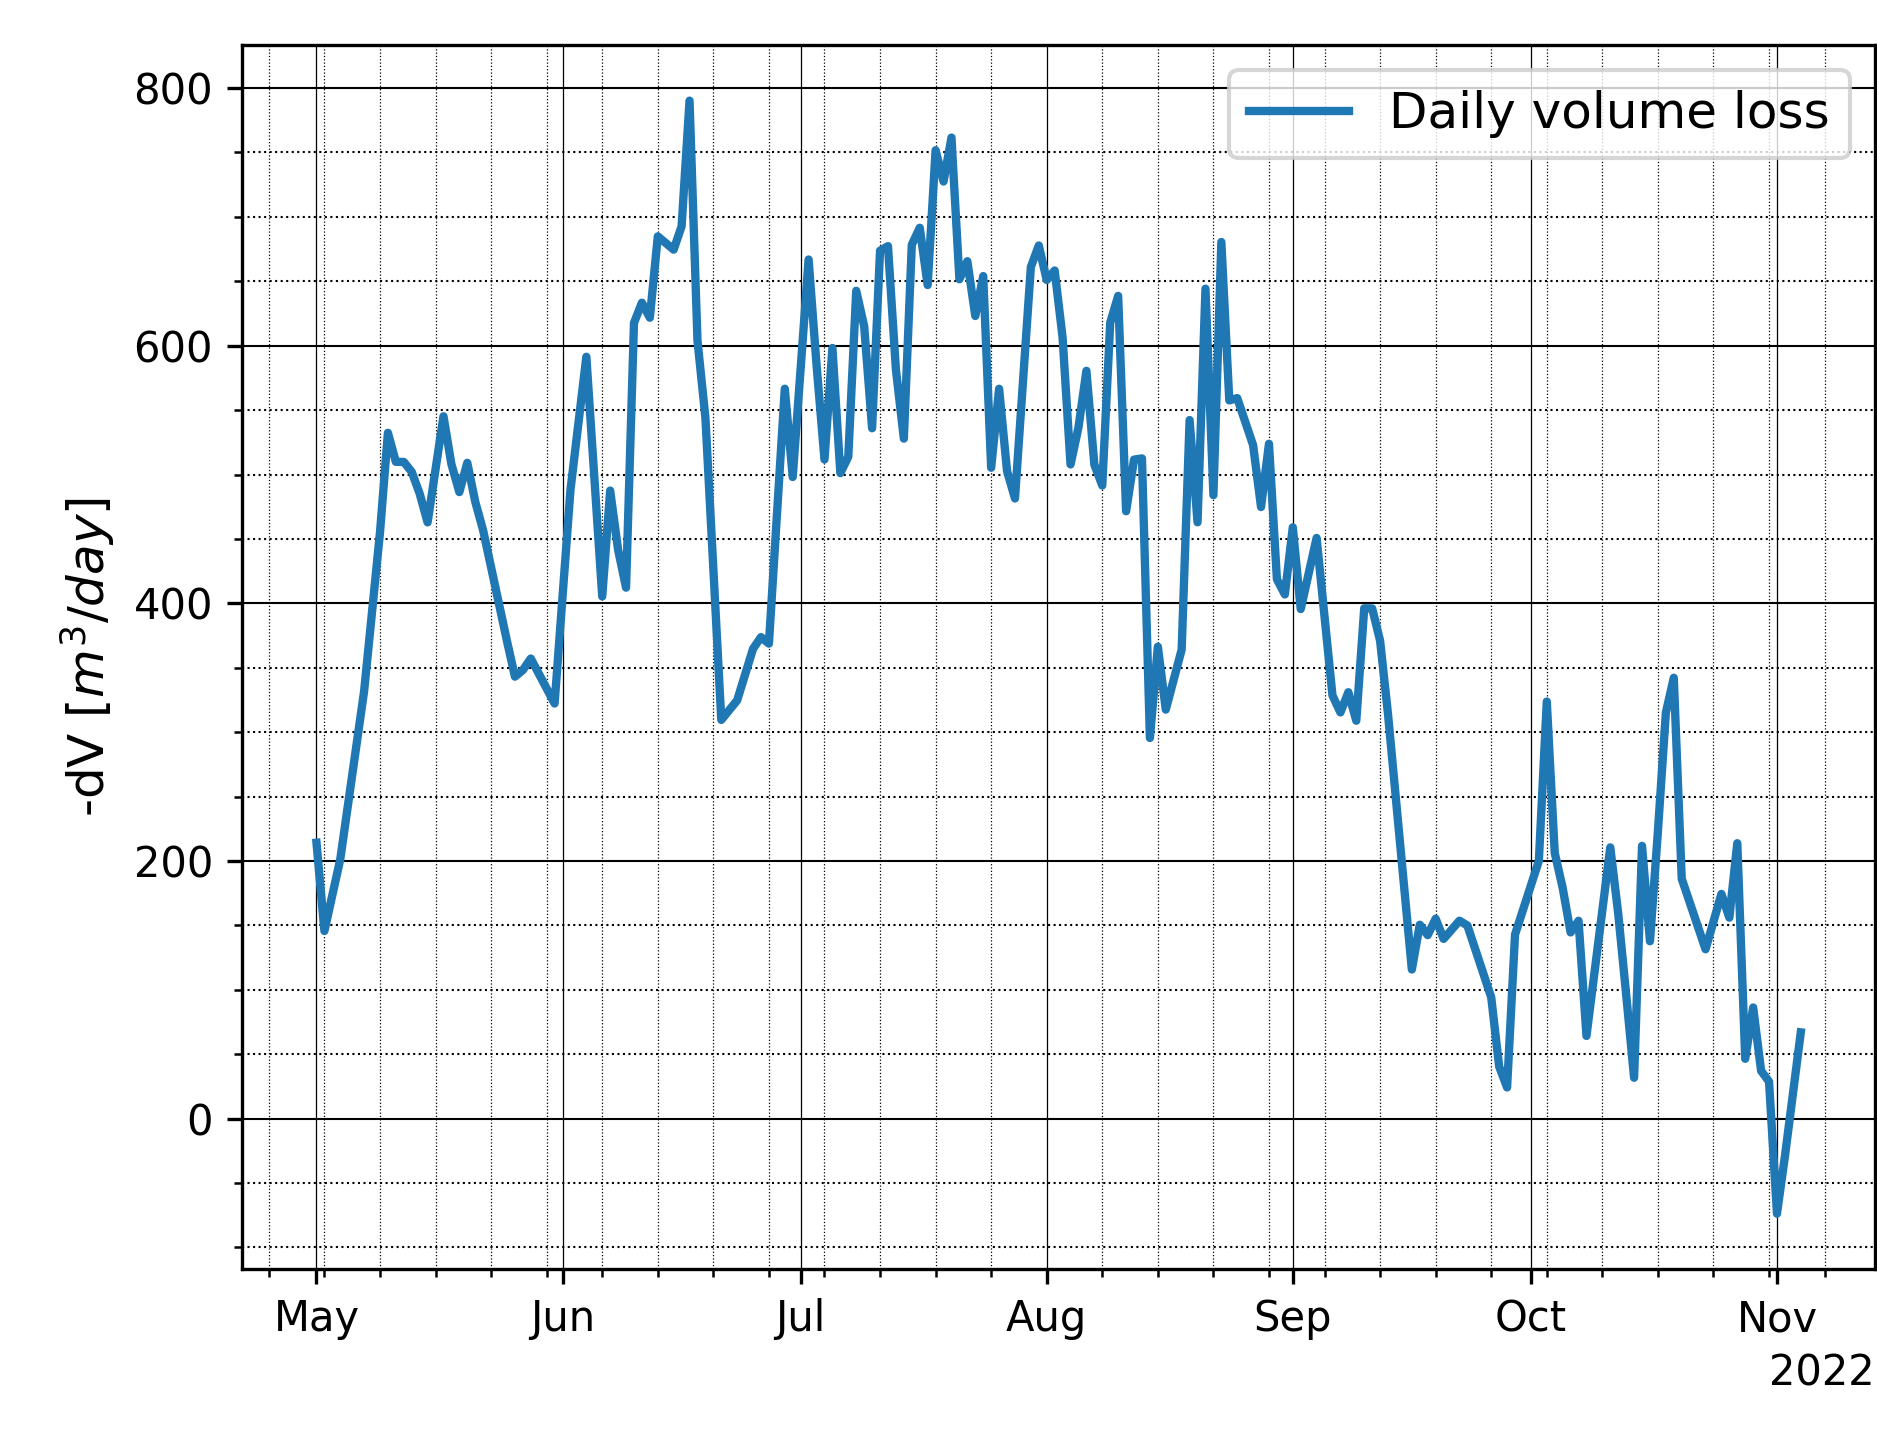
\includegraphics[height=56mm]{4_delta_volumi_stereo_daily.png}
  } 
  \subcaptionbox{\label{fig:4:volumes_variation:cumulated}}{
    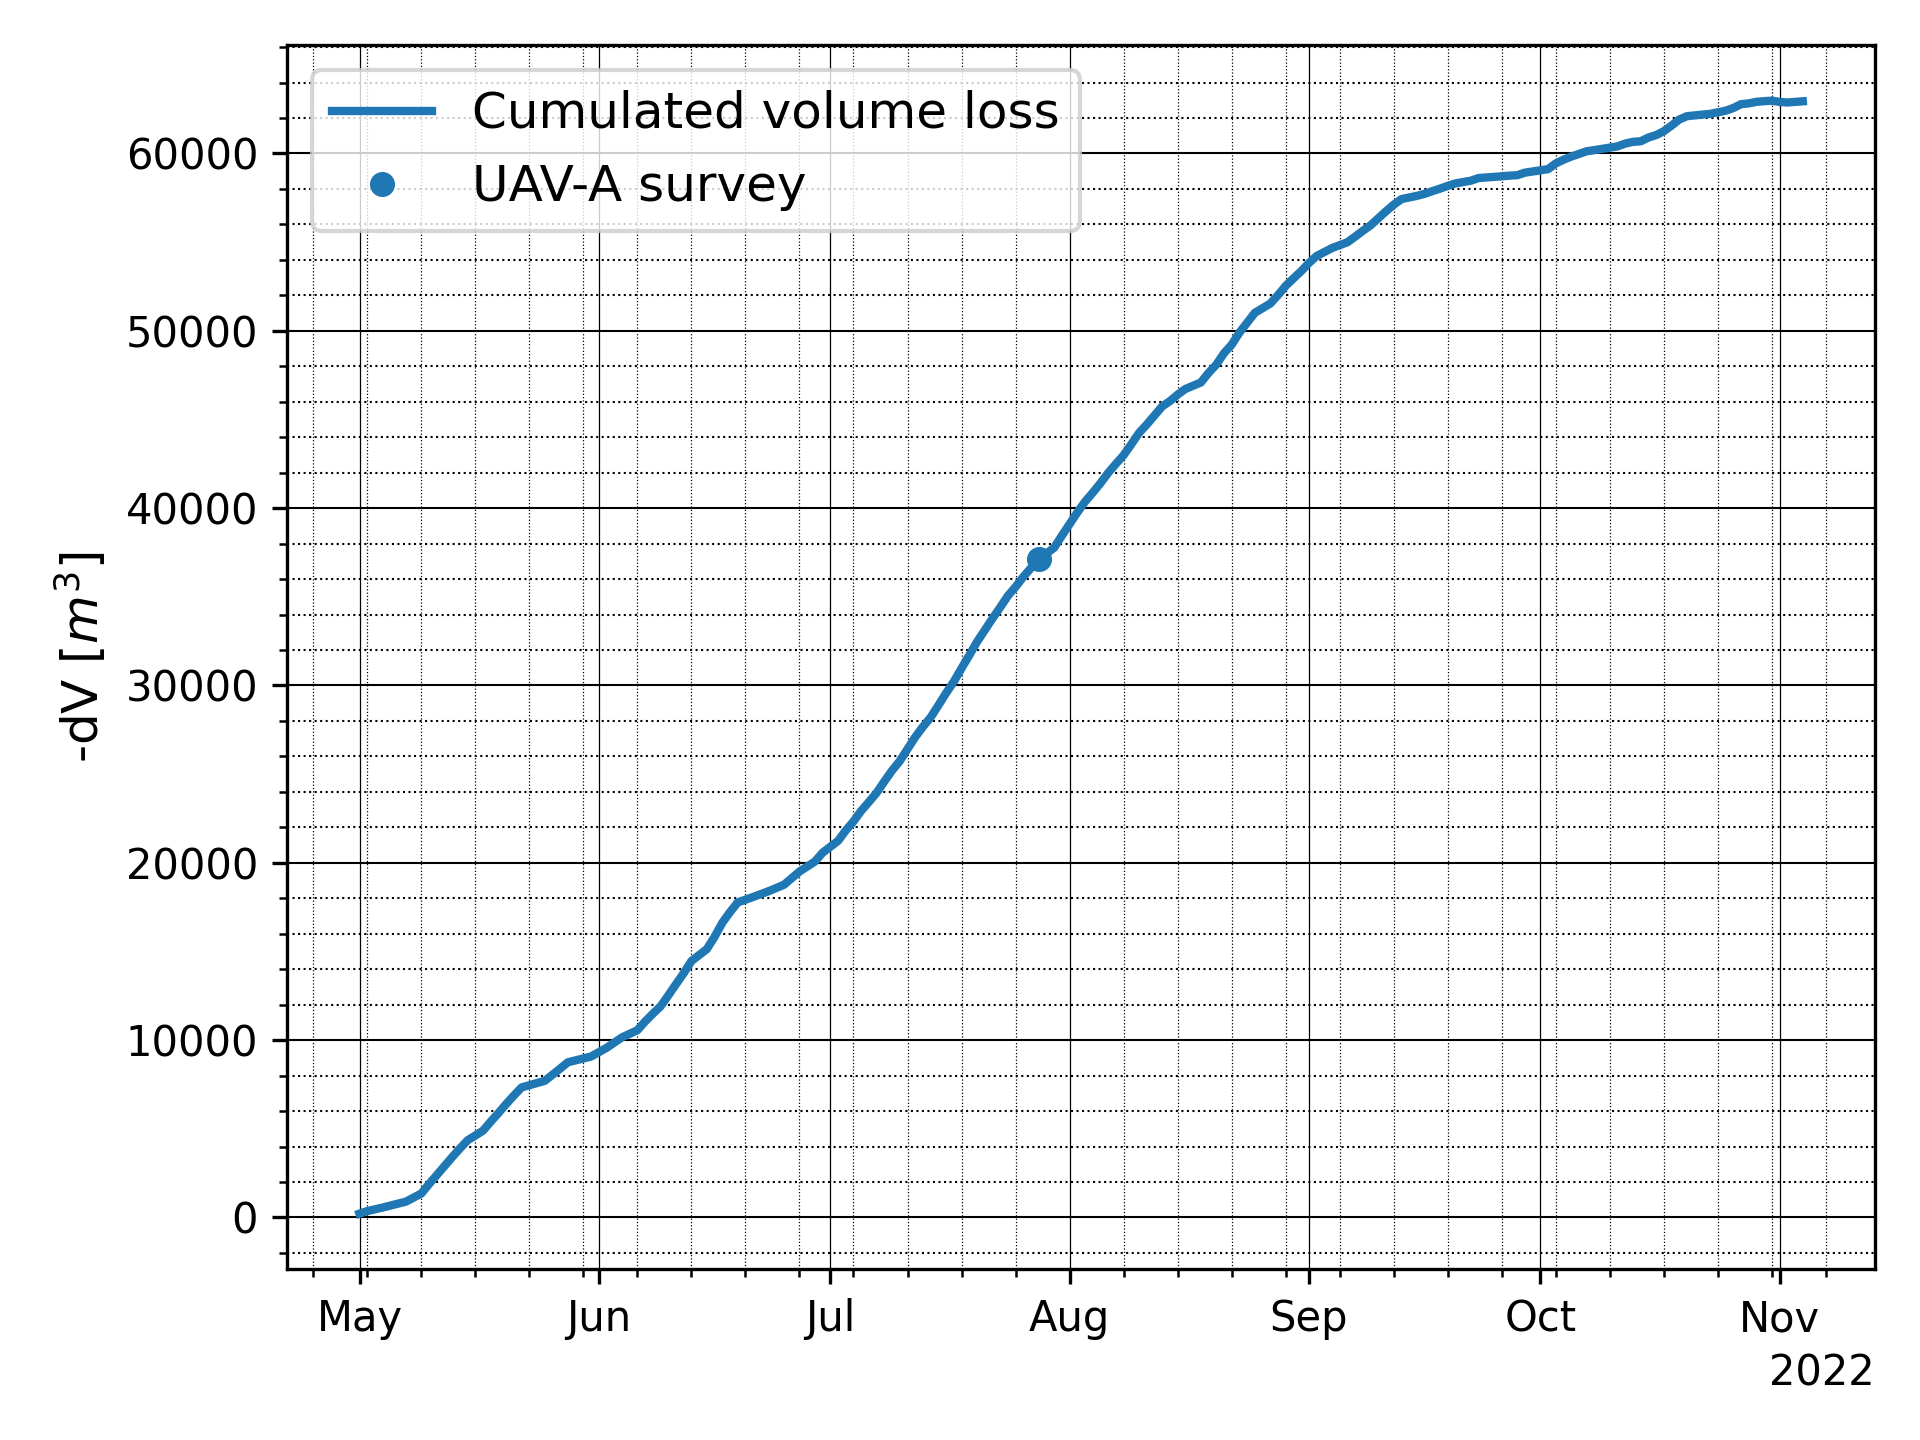
\includegraphics[height=56mm]{4_delta_volumi_stereo_cumlated.png}
  }
  \caption{\textbf{(a)} Daily ice volume lost at the glacier terminus, estimated by DOD of pairs of point clouds spaced by 5 days. \textbf{(b)} Cumulative curve of the ice volume loss during the study period.}
  \label{fig:4:volumes_variation}
\end{figure}

\begin{figure}
  \centering
    \subcaptionbox{\label{fig:4:retrea:map}}{
    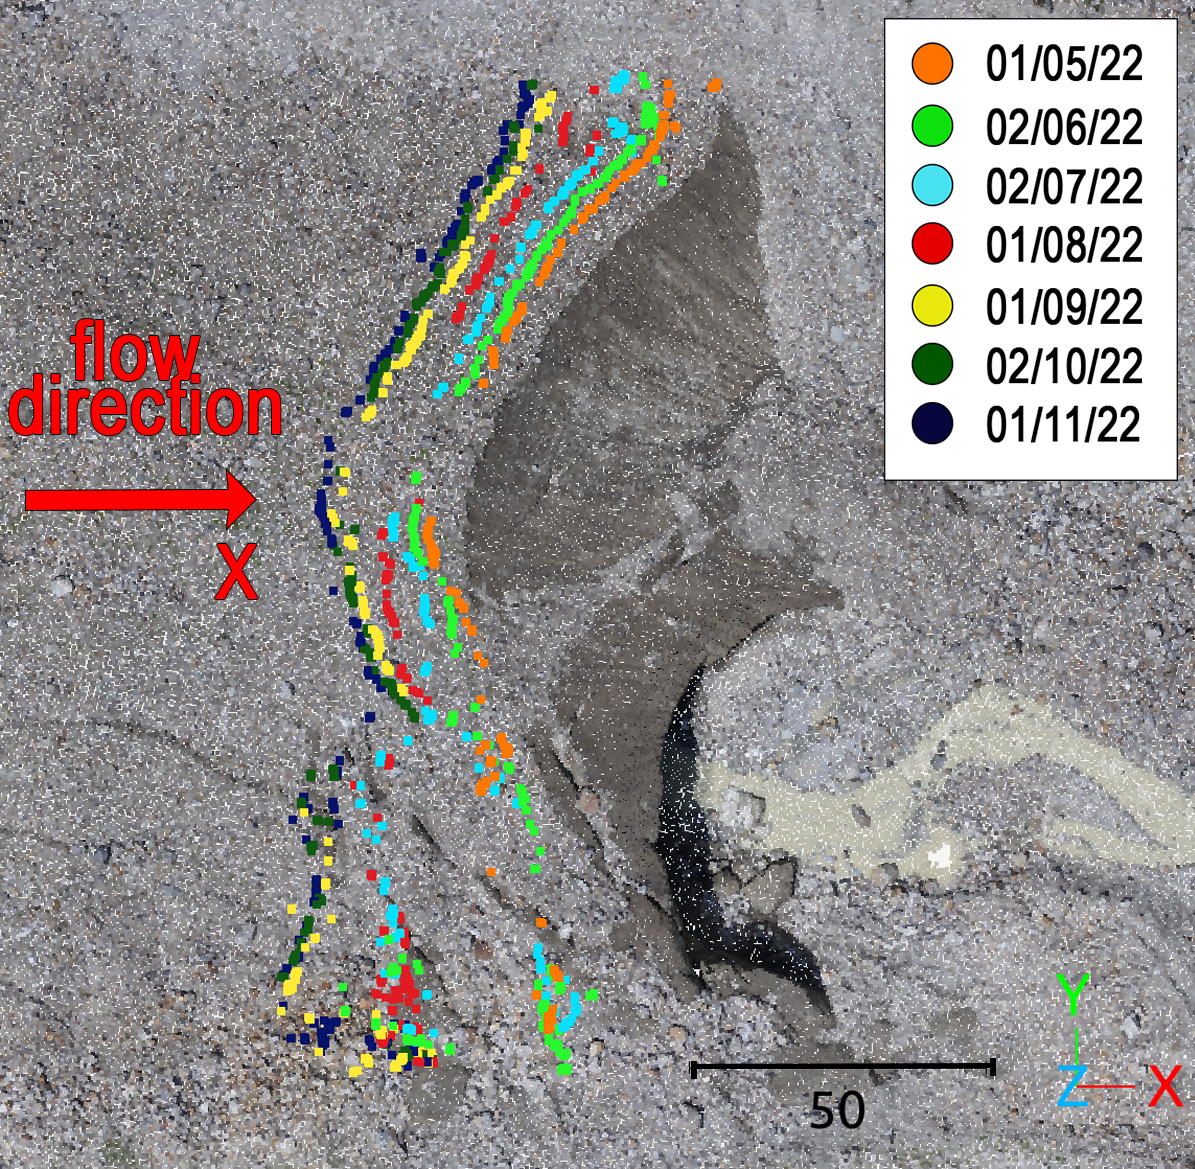
\includegraphics[height=56mm]{4_top_border_series_map.png}
  } 
  \subcaptionbox{\label{fig:4:retreat:ts}}{
    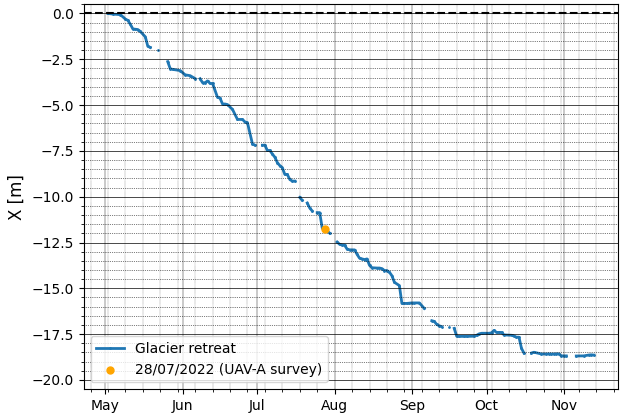
\includegraphics[height=56mm]{4_glacier_retreat.png}
  }
  \caption{\textbf{(a)} Location of the segmented ice cliff top edge at the beginning of each month from May to November 2022; \textbf{(b)} Estimation of daily retreat based on the displacement of the top edge along the flow direction (X-direction). The location of the ice cliff on 01/05/2022 is considered as a baseline for the retreat. The orange marker indicates the day of the UAV-A survey.}
  \label{fig:4:retreat}
\end{figure}

Estimation of ice volume variation was performed by DOD along the
streamwise direction (\secref{sec:4:volumevariation}).
\figref{fig:4:volumes_variation} presents the daily ice volume variations and the cumulated
curve, highlighting the varying ablation rate throughout the study period.
Every value of the time series is referred to as the mean instant between the date of the two point clouds from which it was derived (see~\secref{sec:4:timelag}).
The ice loss rate increases during summer and significantly reduces in autumn,
particularly after mid-September.
A total ice loss of \SI{63000}{\cubic\meter} was observed from 01/05/2022 to 13/11/2022.

The daily glacier was estimated continuously tracking a point located at the center of the top edge of the terminal ice cliff, extracted as described in~\secref{sec:4:topedge}.
The glacier retreat curve is shown in \figref{fig:4:retreat}b and, similarly to that of volume variations, it shows a higher rate of retreat during the summer months, while the retreat velocity decreased between September and November.
From 01/05/2022 to 13/11/2022, a retreat of 17.8 meters was estimated.

\subsection{Validation of the stereo models with UAV data}\label{sec:4:res_uav_validation}

To validate the stereo models, both in terms of internal geometric and absolute
georeferencing errors, the dense stereo point clouds were compared with those obtained from UAV-A (28/07/2022) and UAV-B (05/08/2022) flights.
The signed difference between the UAV point clouds and the stereo point clouds acquired on the same day were computed using the M3C2 algorithm~\citep{lague2013accurate}, in CloudCompare.
M3C2 first computes a 3D local surface normal for each core point at a scale
D, by fitting a plane to the core points located within a radius of size D/2.
Once the normal vectors are defined, the local distance is computed for each core point as the mean distance of the target points that fall inside a cylinder oriented as the normal vector, projected to the cylinder axis.

\begin{figure}
  \centering
  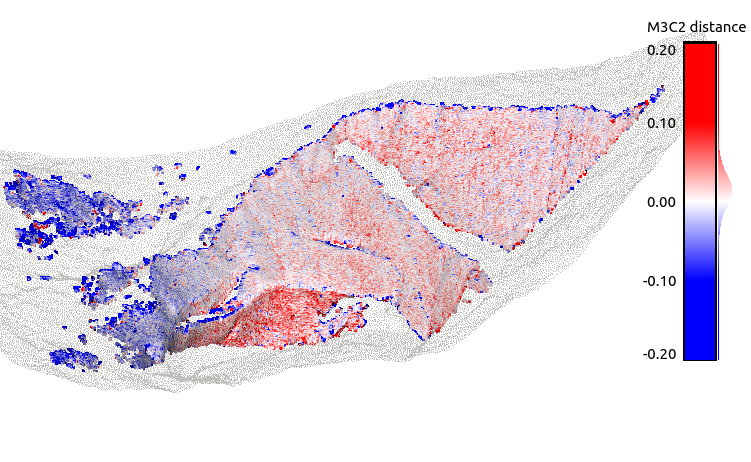
\includegraphics[width=0.8\textwidth]{4_stereo_uav_2807.png}
  \caption{Comparison of the 28/07/22 stereo point cloud with the reference UAV point cloud acquired on the same day, computed with M3C2 algorithm~\citep{lague2013accurate}. The stereo-point cloud is represented with a color scale indicating the distances relative to the UAV point cloud (represented with a light gray color as a reference).}
  \label{fig:4:stereo_uav_2807}
\end{figure}

The comparison with the UAV-A point cloud resulted in a non-significant mean difference between the point clouds of 0.01 m, with a standard deviation of 0.04 cm, indicating an absence of systematic errors in stereo point cloud georeferencing. 
The largest differences were observed at the edges of the stereo point cloud and inside the ice cave \figref{fig:4:stereo_uav_2807}).
Considering the UAV-B block, the mean difference was 0.05 m, with a standard deviation of 0.03 m.
The non-negligible mean difference was likely due to a combination of the georeferencing accuracy of the stereo point cloud and the georeferencing error in the UAV model, which was in the order of a few centimeters (see~\secref{sec:4:uavsurveys}).
UAV-B block, in fact, had limited coverage in the surveyed area and fewer GCPs
compared to UAV-A block.
Overall, both the comparisons showed an overall error of stereo models smaller than 10 cm.
Therefore, a decimetric level of precision can be reasonably considered for the stereo models.

\begin{figure*}[ht]
  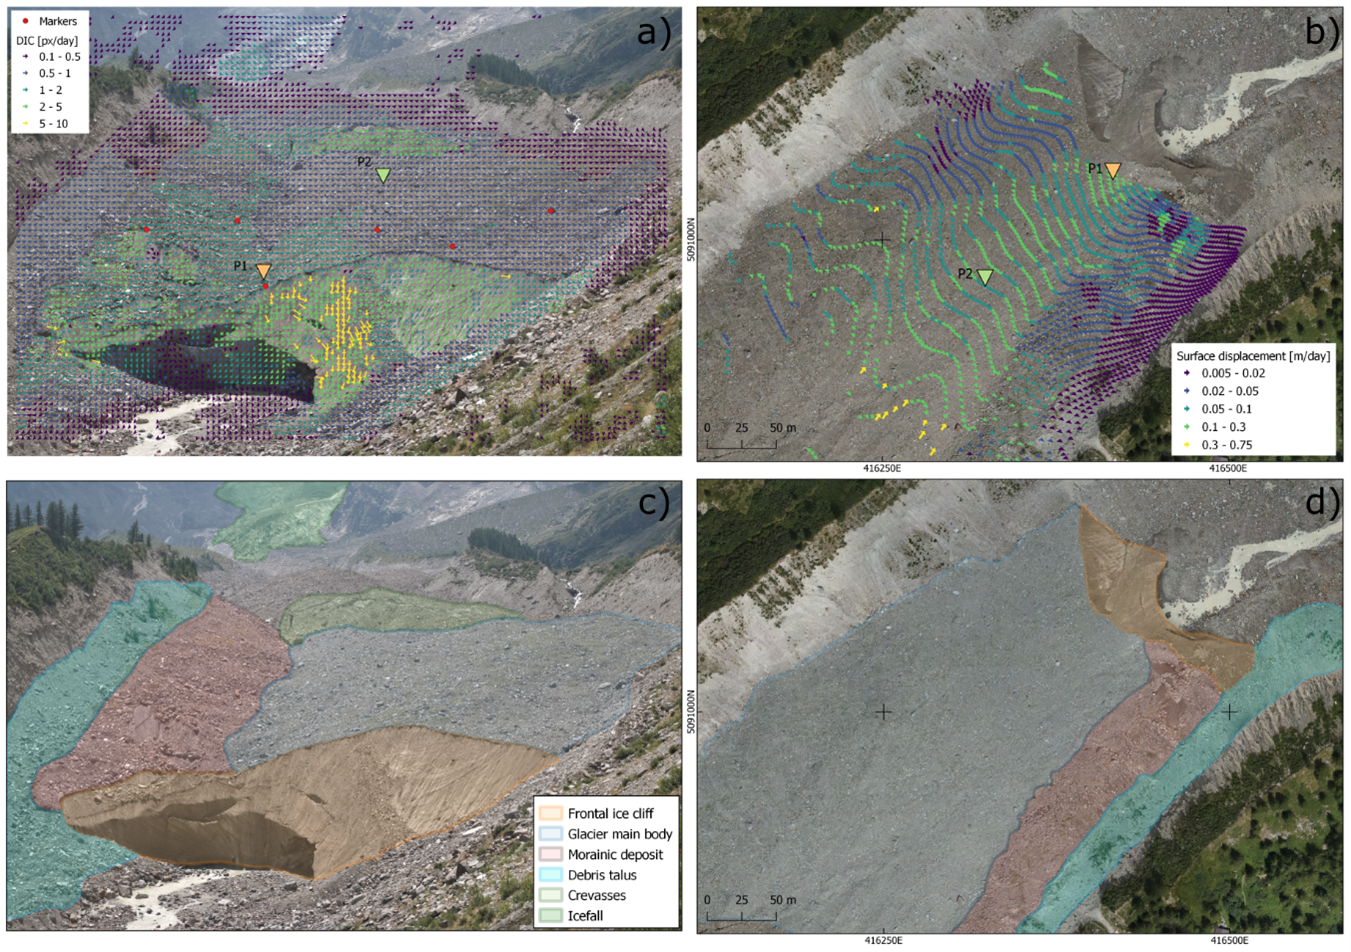
\includegraphics[width=\textwidth]{4_dic_composition.png}
  \caption{(a) DIC displacement map between 25 and 30 July 2022. (b) Orthorectified DIC
    displacement map between 25 and 30 July 2022. The triangles indicate the points P1
    and P2 where we extracted the velocity time series.
    (c, d) glacier domains characterized by specific morphology and kinematics. }
  \label{fig:4:dic_results}
\end{figure*}

\subsection{Glacier surface velocity and morphology}\label{sec:4:res_velocity}

DIC displacement maps allow for evaluating the surface kinematics of the glacier and the
moraines (\figref{fig:4:dic_results}a).
We orthorectified the results only in the area of the right lobe up
to ~1 km of distance from the terminal ice cliff, covering most of the north lobe of the
glacier.
Since the morphology of the frontal ice cliff evolved and moved significantly
during the year, we did not orthorectify the displacement vectors in this area
(\figref{fig:4:dic_results}b).

From the displacement maps of the oblique (\figref{fig:4:dic_results}a,c) and
georeferenced images (\figref{fig:4:dic_results}b,d), it was possible to
identify different domains, based on their morphology and kinematic behavior
(\figref{fig:4:dic_results}c):
\begin{enumerate}
  \item The frontal ice cliff of the glacier, where the ablation process was more
        concentrated. The slope was very steep, and several ice and rock falls occurred,
        particularly at the upper edge, at the limit with the rear part of the glacier.
  \item The debris-covered main body of the glacier, covering the last 400 m of the
        lobe. This region was gentler, and the velocity was higher in the central part.
  \item The lateral morainic deposit, where the lack of lateral pressure from the
        glacier due to the loss of volume destabilized the original moraines. The
        internal part
        collapsed onto the glacier and moved downslope due to glacier traction.
  \item The debris talus resulting from erosional processes on the moraine, where the
        boundary between the glacier and the stable morainic deposit was partially
        covered by a
        debris deposit formed as a result of superficial erosional processes on the steep
        morainic side.
\end{enumerate}

Compared to the glacier's main body, the two latter domains moved at progressively lower
rates, with the morainic talus showing the slowest velocity. Besides the kinematic
regimes, these domains are clearly distinct due to long longitudinal fractures indicating
displacement gradients. In the oblique images (\figref{fig:4:dic_results}c), it
is possible to recognize other portions of the glacier outside the area of interest of
this study, including a lower crevassed area and the icefall that feeds the glacier
lobes.

\begin{figure}[ht]
  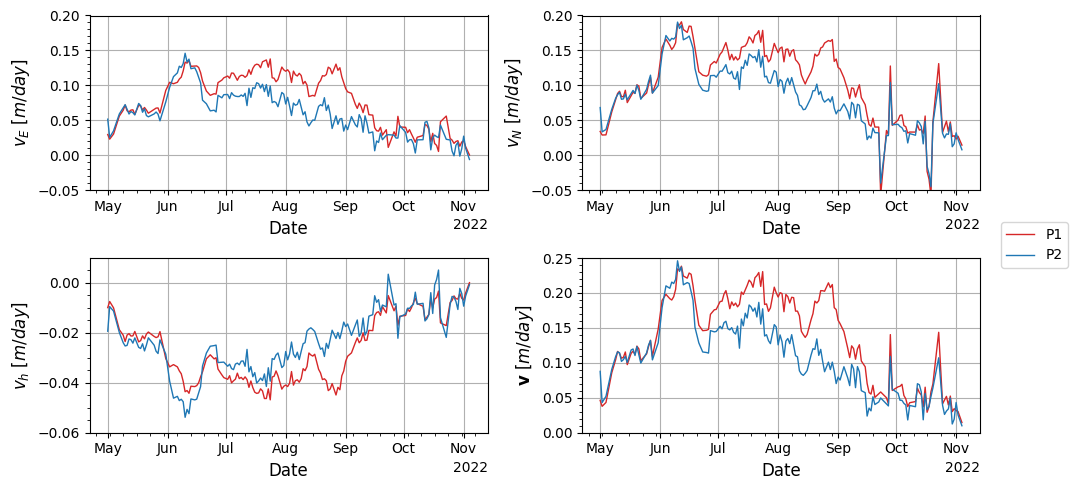
\includegraphics[width=\textwidth]{4_ts_velocities.png}
  \caption{Time series of displacement extracted in the terminal part of the glacier
    lobe. The red curves correspond to point P1, located at 10 m from the terminal ice cliff (considering the location of the terminal ice cliff on 28/07/2022), and the blue curves correspond to point P2 located 120 m far from the ice
    cliff. The location of points P1 and P2 is marked in~\figref{fig:4:dic_results}.}
  \label{fig:4:velocity_ts}
\end{figure}

We considered the displacement time series of two points on the glacier surface: one at
10 meters from the frontal ice cliff at the end of the considered period (P1) and one in
the central part approximately 120 m from the front (P2), as indicated in
\figref{fig:4:dic_results}a,b.
The orthorectified 3D components of daily velocity and the velocity module, calculated
between pairs of images spaced 5 days apart (see \secref{sec:4:timelag}), are shown in
\figref{fig:4:velocity_ts}.
The time series exhibit similar behavior, with a Spearman correlation coefficient
of 0.88, and show comparable velocity values between May and the first half of June and
from the second half of September until the end of the period.
However, P1 has a ~30\% higher velocity during the warm season, with values ranging from
\SI{0.15}{\meter\per\day}, occurring on a few days during the second week of August and
at the beginning of September, to \SI{0.23}{\meter\per\day} in mid-July.
The South-North velocity component is the highest, varying during the warm season between
\SI{0.10}{\meter\per\day} to \SI{0.18}{\meter\per\day} (P1) and \SI{0.06}{\meter\per\day}
to \SI{0.15}{\meter\per\day} (P2).
The East-West component is approximately \SI{0.05}{\meter\per\day} lower, while the
vertical component assumes smaller values, approximately \SI{0.03}{\meter\per\day}.

\begin{figure}[ht]
  \centering
  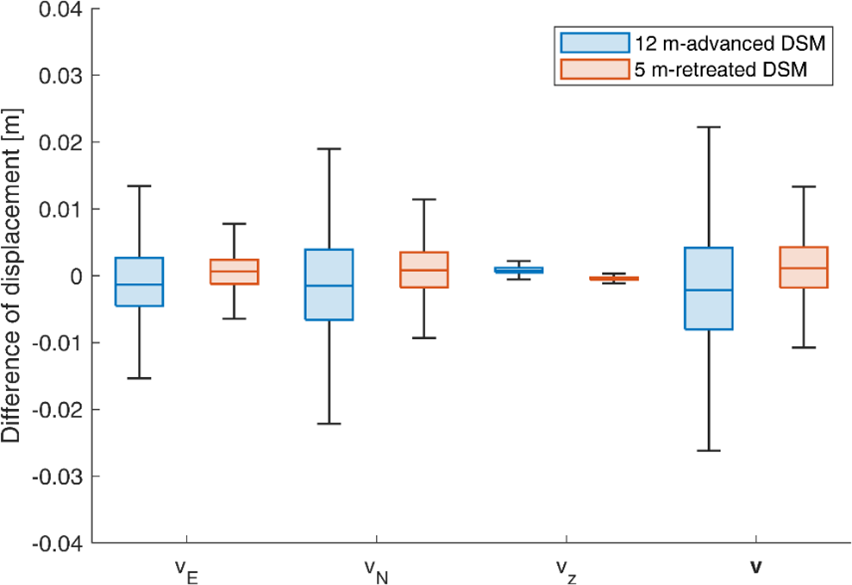
\includegraphics[width=0.7\textwidth]{4_velocity_ortortect_uncertainty.png}
  \caption{Uncertainty analysis of velocity vector orthorectification against possible
    DSM variation. Blue boxes represent the difference between the velocity vectors
    back-projected on the true DSM of 28/07/2022 and those back-projected on a simulated
    DSM advanced downstream by 12m (as it was in May 2022).
    Red boxes represent the difference between the true velocity vectors and those
    obtained with a simulated DSM with the glacier front retreated 5 meters upstream
    (as it was in November 2022).
    \(v_E\), \(v_N\), \(v_z\), and \(v\) are respectively the three components in the
    east, north, and height directions and the magnitude of the differences of the
    velocity vectors.
  }
  \label{fig:4:velocity_ortortect_uncertainty}
\end{figure}

\subsection{Velocity orthorectification uncertainty}\label{sec:4:res_velocity_uncertainty}

To estimate the error related to DSM variations, we simulated two different snout
positions, as described in \secref{sec:4:orthorectification_uncertainty}.
The first simulated snout position was 12 meters
downstream of the location of the terminal ice cliff on 28/07/2022, which was the most
advanced front position at the beginning of the season
(\figref{fig:4:retreat}b).
The second simulated snout position was 5 meters upstream, representing the most
retreated position at the end of the season (\figref{fig:4:retreat}b).
On average, the different front locations caused a glacier elevation change of
\SI{+1.76}{\meter} and \SI{-0.88}{\meter} for the advanced
and retreated positions, respectively.
The differences between the velocity vecotors orthorectified with the true and the
simulated DSMs are
summarized in \figref{fig:4:velocity_ortortect_uncertainty}.
The considered velocity vectors were measured by DIC between 25 and 30 July 2022, during
a five-day period centered around the acquisition of the UAV-A DSM of 28/07/2022.
It was observed that the velocity vertical component \(v_h\) was the least influenced,
with a normalized MAD\(_z\) of \(2.6\%\) for
the advanced simulated position and \(1.3\%\) for the retreated position. The MADs of the
East and North planimetric components \(v_E, v_N\) were similar and approximately \(2.5\)
times higher than MAD\(_z\), while the normalized MADs of the velocity modules were
\(5.2\%\) and \(2.6\%\) (advanced and retreated positions).

\begin{figure}[ht]
  \centering
  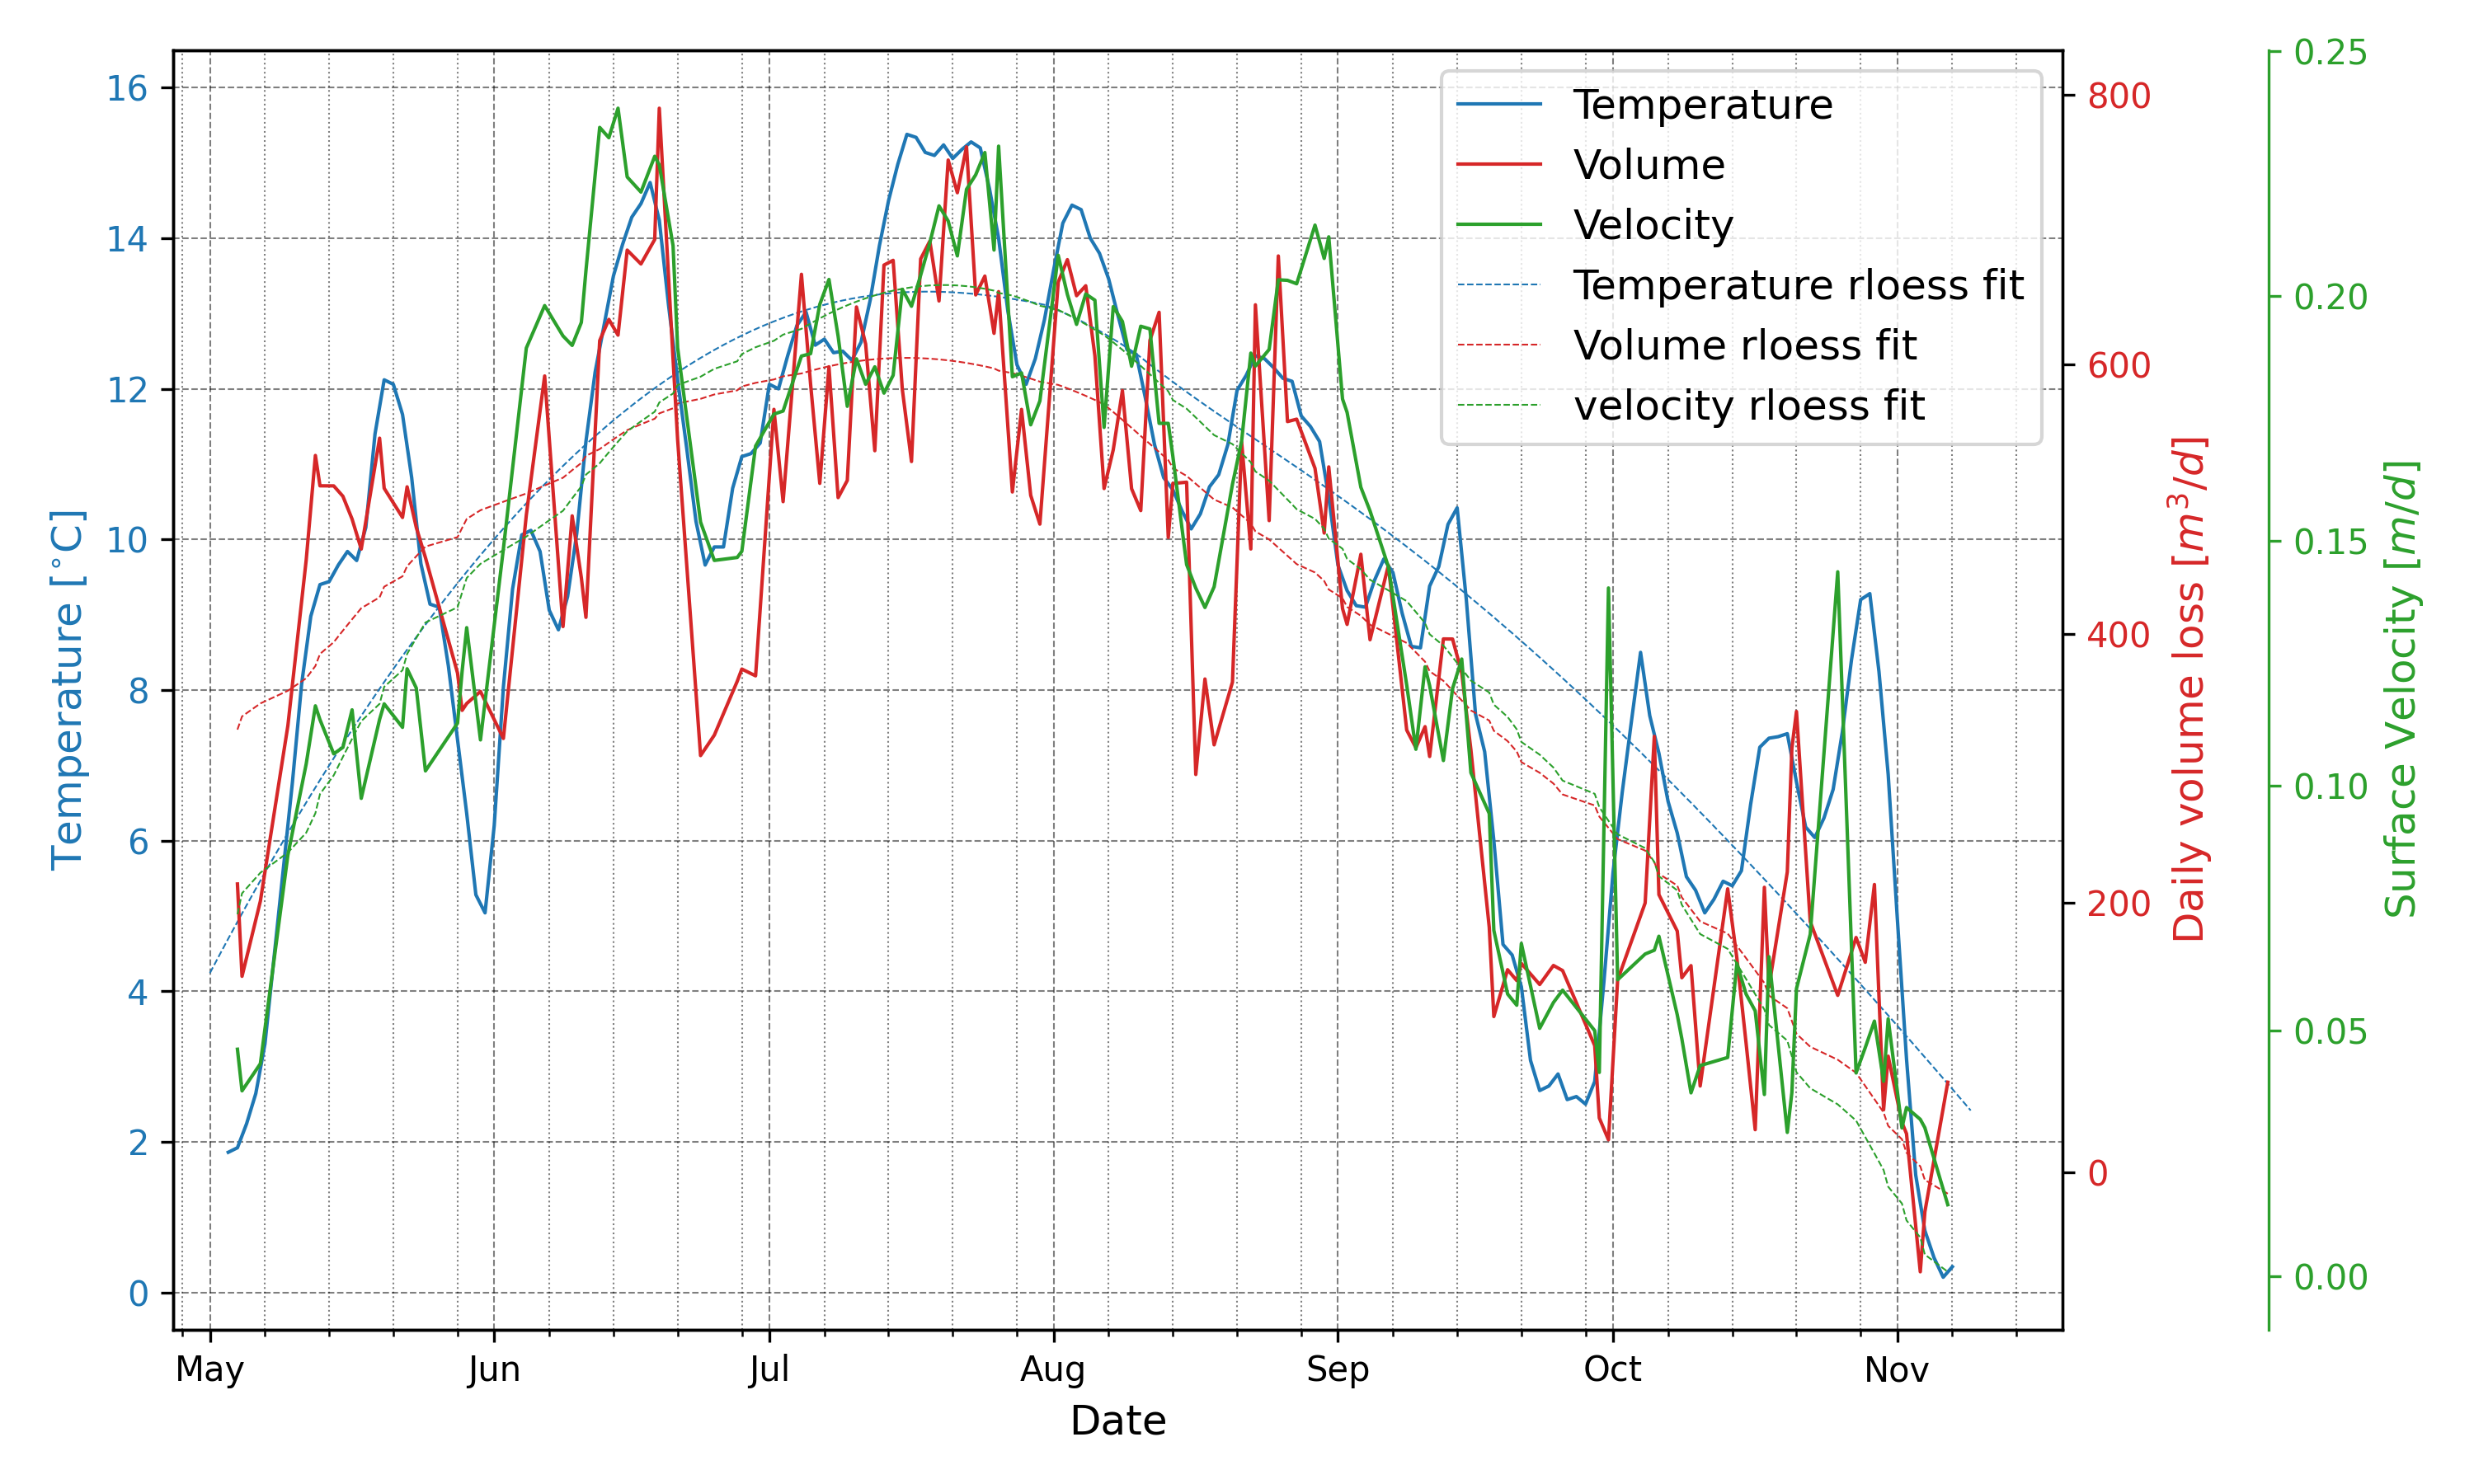
\includegraphics[width=1\textwidth]{4_TS_P1.png}
  \caption{Time series of the daily volume loss due to the glacier terminus retreat,
    compared to the time series of glacier surface velocity extracted by monoscopic DIC at the location of point P1 (located close to the ice cliff terminus and marked with an orange triangle in~\figref{fig:4:dic_results}) and the 5-day smoothed time series air temperature measured by the AWS at the location marked in~\figref{fig:4:studyarea}.}
  \label{fig:4:TS_punto-fronte}
\end{figure}

\subsection{Comparison between surface velocity, frontal ice loss and meteorological
  variables}\label{sec:4:res_temp_comparison}

We compared the time series of ice volume variation \(dV\), obtained with the stereo
cameras, and the magnitude of the surface velocity \(v\) obtained by the monoscopic
camera approach at the locations of points \(P1\) and \(P2\) (labelled as
\(\mathbf{v}_{P1}\) and \(\mathbf{v}_{P2}\)) with the series of daily
meteorological measurements acquired by the AWS.
We observed a significant relationship between the daily average air temperature \(T\),
glacier surface velocity, and volume variations, while precipitation and incoming solar
radiation were decorrelated. \figref{fig:4:TS_punto-fronte} shows the time series and
the seasonal trend.
All the series exhibit the same behavior, which is in phase.
To remove the main seasonal trend and analyze the detrended signal, we subtracted the
robust
loess fit~\citep{Cleveland1979} from the original series and computed the Spearman
correlation coefficients for each pair of variables
(\tabref{tab:4:correlation_coefficients}).
The correlations were always larger than \(0.49\) for the detrended signal and larger
than \(0.81\) for the original series.

\begin{table}
  \centering
  \caption{Spearman correlation coefficients between original (\(\rho_S\))
    and detrended \(\rho_D\) signals for the daily volume variation (\(dV\)), mean air
    temperature
    (\(T\)), and surface velocity of points \(P1\) and \(P2\) (\(\mathbf{v}_{P1}\) and
    \(\mathbf{v}_{P2}\) respectively).
    In all the cases, the p-value was \(< 10^{-5}\).}
  \label{tab:4:correlation_coefficients}
  \begin{tabular}{lcc}
                                               & \(\rho_S\) & \(\rho_D\) \\
    \hline\noalign{\smallskip}

    \(dV\) \& \(T\)                            & 0.89       & 0.80       \\
    \(dV\) \& \(\mathbf{v}_{P1}\)              & 0.87       & 0.64       \\
    \(dV\) \& \(\mathbf{v}_{P2}\)              & 0.81       & 0.49       \\
    \(T\) \&  \(\mathbf{v}_{P1}\)              & 0.88       & 0.59       \\
    \(T\) \&  \(\mathbf{v}_{P2}\)              & 0.82       & 0.59       \\
    \(\mathbf{v}_{P1}\) \& \(\mathbf{v}_{P2}\) & 0.88       & 0.64       \\
    \noalign{\smallskip}\hline
  \end{tabular}
\end{table}

\section{Discussion}
\label{sec:4:discussion}

\subsection{Hand-crafted vs deep learning matching}\label{sec:4:handcrafted_vs_dl}

In the case of the Belvedere Glacier, the wide baseline between the two cameras posed a
challenge for traditional hand-crafted matching techniques, which failed to find
sufficient corresponding points for estimating camera poses.
Traditional feature matching, including well-known commercial solutions like
Agisoft Metashape, yielded a limited number of poorly distributed tie points, ranging
from a dozen to a hundred of tie points.
In all the cases, the tie points were concentrated mainly in the central part of the ice
cliff, where the ice cliff was nearly vertical, and it was not possible to determine
camera relative orientation.

On the other hand, DL feature matching algorithms outperformed traditional hand-crafted
methods, successfully finding a significant number of corresponding features.
SuperPoint and SuperGlue matched between 1000 and 3500 features, which were
well distributed over the entire ice cliff with some along the streamwise right moraine
in the background.
This substantial matching success allowed for estimating a sparse but complete 3D
reconstruction of the terminal ice cliff, serving as the starting point for a
dense scene reconstruction.
With a reliable camera pose and sparse reconstruction in place, traditional dense
matching algorithms, like semi-global matching, proved to be effective.
To further enhance the result, state-of-the-art algorithms can be employed for
even better performance.

\subsection{Merging stereoscopic and monoscopic processings to study the glacier
  dynamics}\label{sec:4:stereo_monoscopic}

The stereoscopic and monoscopic workflows focused on different aspects of the glacier's
dynamics and the combined use of these two information is useful for the characterization
of the glacier behavior of the studied area.
The installation of two cameras allowed for the stereoscopic reconstruction of the
glacier snout and the computation of volume variations, while the use of a single camera
(C2) allowed for the characterization of the movement of the debris-covered sector of the
lobe.

The proposed system was able to monitor the evolution of the glacier in its different
sectors and supports the identification of different kinematic sectors
(\figref{fig:4:dic_results}).
The north lobe of the Belvedere Glacier exhibited a complex motion that involves multiple
components.
This included a retreat along the streamwise direction, a downslope forward motion due to
glacier sliding, and a thinning of the glacier surface caused by ablation.
From the stereoscopic processing, it was possible to extract morphology and position of
the terminal lobe, which retreated of 17.6 m between May and November 2022
(\figref{fig:4:retreat}), and ice volume loss (\figref{fig:4:volumes_variation}).
On the other hand, the monoscopic approach allowed to derive the forward motion of the
glacier, by tracking features on the glacier surface.
Additionally, the availability of volumetric and kinematic data allowed
the combined analysis of potential relationship between volume variation, surface
velocity and external meteorological factors such as air temperature.

\subsection{Glacier velocity, frontal ablation and
  temperature}\label{sec:4:discuss_velocity_ablation_temperature}

Typically, mountain glacier motion is dominated by basal sliding~\citep{willis1995intra},
which is related to the state of the hydraulic drainage
system~\citep{vincent2016sliding}.
In particular, the water pressure is higher in the presence of distributed small
channels~\citep{pimentel2011numerical}, while it diminished when large cavities form and
a more
efficient drainage develops~\citep{nienow2005hydrological}.
As a consequence, glaciers flow is often faster in early summer than at the end of the
warm season~\citep{sanders2018variations,vincent2016sliding}.
Therefore, at seasonal scale, glacier surface velocity is sometimes not linked to air
temperature~\citep{sanders2018variations}.
At hourly to daily scale, several studies showed that the flow velocity is linked to
subglacial water pressure \citep{sugiyama2010surface} and air
temperature~\citep{liu2019diurnal},
even though~\citet{allstadt2015observations} did not observed a significant variation in
the diurnal cycle.
Moreover, in many cases the flow velocity was observed to rise after intense
rainstorms~\citep{benoit2015multi,horgan2015glacier,sugiyama2010surface}.

We showed that the daily air temperature variations are strictly linked to glacier
surface velocity at a daily to weekly scale.
On a monthly scale, we registered the highest velocity in July, even though the absolute
peak was reached in the first half June, concurrently with high air temperature.
Contrary to the findings of other
scholars~\citep{benoit2015multi,horgan2015glacier,sugiyama2010surface}, we did not
register any relationship with rainfall episodes.
These observations suggest that (at least in the lower portion of the north lobe) the
subglacial hydraulic system remained homogeneous during the season.
Besides, we also observed an even stronger relationship of the air temperature with the
frontal ablation, which, to our knowledge, has never been documented before.
This was possible thanks to the stereoscopic system that produced volumetric data,
increasing the understanding of the glacier snout dynamics.

\subsection{Transferability of the system}\label{sec:4:transferability}

The transferability of the low-cost camera system used in this study to other test sites
is a crucial aspect to consider.
The installation process of the system is relatively straightforward as the cameras are
mounted on topographic tripods, eliminating the need for complex and permanent
structures.
This ease of installation enables the system to be replicated in different sites without
significant difficulty.
While a more robust installation with minimal vibrations and camera rotations would be
beneficial, the simplicity of the setup allows for efficient deployment by a small team,
without the requirement of specialized equipment.

The Belvedere glacier, characterized by debris cover and a dirty ice terminal cliff,
presents favorable conditions for 3D reconstruction due to the presence of distinct
patterns in the images.
However, successful 3D reconstructions of bare ice or snow-covered areas have also been
achieved in previous studies.
\citet{belloni2023} and~\citet{Gindraux2017} utilized UAV-SfM to generate 3D models
of debris-free or partially debris-covered glaciers.
\citet{Taylor2023} demonstrated the effectiveness of an extremely low-cost camera for 3D
reconstruction of a debris-free glacier calving front in Iceland.
Additionally,~\citet{Avanzi2018} and~\citet{DeMichele2016} employed UAV-based
photogrammetric reconstruction to map snow depth Despite snow having even fewer
discernible patterns than bare ice, the use of multi-camera photogrammetry allowed for
achieving accurate 3D reconstructions.
It is worth noting that these examples utilized traditional feature matching techniques.
With state-of-the-art DL sparse and dense matching techniques, results can be further
improved.
Even though the Belvedere glacier's characteristics facilitate 3D reconstruction,
successful reconstructions of debris-free ice and snow-covered areas using similar
techniques have been demonstrated in the literature, supporting the broader applicability
of the low-cost camera system for monitoring glaciers in diverse environments.

% References
\makechapterbibliography{}
